\chapter{Experiment of Rivet-HSB Hybrid Connection}
\label{ch3}

%%%%%%%%%%%%%%%%%%%%%%%%%%%%%%%%%%%%%%%
% IMPORTANT
\begin{spacing}{1.25} %THESE FOUR
\minitoc % LINES MUST APPEAR IN
\end{spacing} % EVERY
\onehalfspacing % CHAPTER
% COPY THEM IN ANY NEW CHAPTER
%%%%%%%%%%%%%%%%%%%%%%%%%%%%%%%%%%%%%%%
\section{Introduction}


Rivets were widely used in the world to fasten steel members in the early days, and also used for cross-section connections for steel bridges. Since 1950, countries worldwide have been issued design specifications for high-strength bolts connection, and high-strength bolts connection have gradually replaced rivet connections. However, many riveted bridges are still in service \cite{Collette2014Experimental1880s1890s}. Some of the rivets might be corroded and loosen due to deterioration of the paint coating. The reduction of the volume of a rivet's head is severely affected fatigue life \cite{Heinemeyer2011TheConnections}. Studies have also pointed out the influence of rivets' material loss on these bridge structure elements' remaining bearing capacity \cite{Hashimoto2010,Macho2016}. For structural performance recovery or to extend their service life, the riveted bridges have to repair or reinforce by replacing the corroded rivets with high-strength bolts. Replacing the rivets with a high-strength bolt for changing to the frictional joint is a desirable approach to repairing the corroded riveted joint \cite{KOMATSU2015}.
    
Applying such repair, whether it satisfies the frictional joints' performance requirements depends on the slip coefficient. However, the riveted joint surface's slip coefficient with red lead paint for corrosion is not specified. Therefore, giving a proper evaluation of the slip coefficient is one of the purposes of this paper.
Lead is an excellent anti-corrosive, lead-based paint that could be well protecting a steel structure from the element. Especially red lead (Pb3O4) was once widely used for bridges anti-corrosion paint. However, Lead-based paint has been a significant cause of lead poisoning. Countries around the world are beginning to call for an end to the use of Lead-based paint. \ac{CPSC} has already started banning lead-based paint in 1977 \cite{CPSC1977}. In 1987, Japan completely stopped using red lead as anti-corrosion paints for steel structures \cite{rtri1987Steel}. So far, the use of red lead has been completely discontinued and replaced by inorganic resin coatings. Red lead and rivets are used on steel bridges almost in the same period. Since rivets are designed to transmit load by shearing force, the friction performance of riveted joint surfaces with red lead paint is unspecified. 

In this study, the authors have got the opportunity to obtain a 90-year-old riveted bridge's cross-beam. The joint part was cut out from this bridge's cross-beam and evaluated the riveted joint surface's aging condition in natural corrosion weakening by microscope observation and elemental analysis. In addition, the small-scale slip test is conducted to investigate the joint surface's slip coefficient of the riveted joints experimentally. Finally, the pressure distribution test is conducted using a pressure measurement film to explore the pressure distribution and the effective contact pressure area of riveted joints' surface.

The girders of steel riveted bridges are often thin plates and the same applies to the joints. For riveted joints, the joint bearing capacity is generally determined by the rivet/main plate bearing pressure or the shear of the rivet, but it may also be determined by the yielding of the main plate. This study investigates repair and reinforcement methods for riveted joints where the main plate is yield-precedent (thin plate), by replacing the rivets with high-strength bolts.

The following three methods can be used to repair rivets that have corroded due to age-related deterioration. The following three methods can be identified as methods of repairing rivets that have corroded due to age: (1) replacement with new rivets, (2) high-strength bolt support joints, and (3) replacement with high-strength bolt friction type joints. However, the application of method (1) is difficult due to the fact that few construction engineers are available. Therefore, replacement with a support high-strength bolt is the most promising method. However, the adoption of a support joint is difficult to control the hole diameter, and from the viewpoint of reliable construction on site, the most promising method is the replacement with a high-strength bolt for friction bonding. In addition, from the viewpoints of economy and workability, partial replacement is often considered preferable to total replacement. In this study, joint tensile tests are carried out to determine the load carrying capacity of existing riveted joints when partially or fully replaced with high-strength bolts for friction joints, and the slip coefficient that can be expected in the design.


\section{Slip coefficient of riveted joint}



\subsection{Joint faying surface's aging condition}

The bridge of the research object has been in use for 90 years. The bridge's paint was probably damaged, and the joint surface was probably corroded due to aging. In order to investigate the condition of the aging bridge joint's surface, 40mm x 40mm compact specimens cut out from the joint to conduct microscope observation, Fourier-transform infrared spectroscopy analysis (FT-IR), and \ac{EDX} analysis.

\subsubsection{Microscope observation} \label{ch3sec2-1}

Depending on where the specimen was taken out, the red lead's aging condition has been found different. The research has shown that the red lead paint adjacent to the rivet hole has been compromised due to high temperature and clamping force by riveting. The friction coefficient may be affected by this \cite{Leonetti2020RivetBridges}.

The red lead on the joint surface has partly peeled off, and the black oxide of the steel can be observed, which indicates that the red lead's adhesion has become poor over aging, as shown in Fig. \ref{ch3fig2b}

\begin{figure}[htbp]
    \centering
    \begin{subfigure}[t]{0.4\textwidth}
    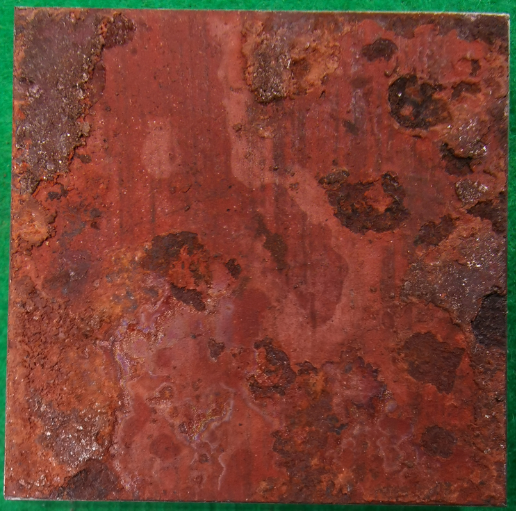
\includegraphics[width=\linewidth]{imgs/ch3/fig2a.png}
    \caption{Normally}
    \label{ch3fig2a}  
    \end{subfigure}
    \hfill
    \begin{subfigure}[t]{0.4\textwidth}
    
\includegraphics[width=\linewidth]{imgs/ch3/fig2b.png}
    \caption{Seriously}
    \label{ch3fig2b}  
    \end{subfigure}
    \caption{Faying surface for riveted joint}
\end{figure}

As shown in Fig. \ref{ch3fig3}, the joint surface was observed with an electron microscope of 50 times and 600 times, more detailed diagrams will be listed in Appendix \ref{app-obsur}. The orange-red substance is red lead, and the black primer is the black oxide of steel. No obvious traces of rust are found on the joint surface. The light reflecting material in the picture is a resin coating, and it will be confirmed by elemental analysis for the next section.

\begin{figure}[htbp]
    \centering
    \begin{subfigure}[t]{0.4\textwidth}
    
\includegraphics[width=\linewidth]{imgs/ch3/fig3a.jpeg}
    \caption{50X}
    \label{ch3fig3a}  
    \end{subfigure}
    \hfill
    \begin{subfigure}[t]{0.4\textwidth}
    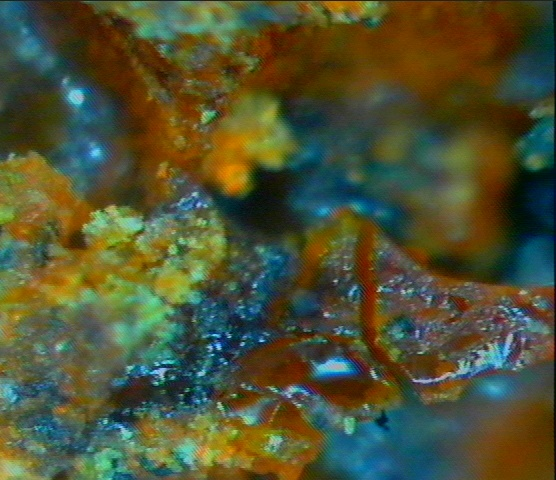
\includegraphics[width=\linewidth]{imgs/ch3/fig3b.jpeg}
    \caption{600X}
    \label{ch3fig3b}  
    \end{subfigure}
    \caption{Microscope observation}
    \label{ch3fig3}
\end{figure}

\subsubsection{FT-IR and EDX analysis}

This study randomly selected three specimens from different positions of the joint and conducted FT-IR analysis on the joint surface. Furthermore, the presence of elements on the joint surface detected by EDX analysis. FT-IR spectra of the joint surface are illustrated in Fig. \ref{ch3fig4}. The spectrum consists of many sharp and weak bands in the region of 700–900 cm-1, in addition to a few bands in the region of 1,500–2,000 cm-1. Most of the main peaks corresponding to vinyl acetate (C4H6O2) were detected \cite{baskaran2004Vibrational}, but no main peaks corresponding to Iron (III) oxide (Fe2O3) were found. The study has shown that incorporating various metallic additives into polymer matrices can produce polymer-matrix composites and improve their properties for specific applications \cite{dong2006Polyvinylbutyral}. In order to enhance the adhesion of red lead, a resin-based primer is usually applied before the red lead. It can be considered that the vinyl acetate detected by FT-IR acts as a resin-based primer to enhance the adhesion of red lead.

\begin{figure}[htbp]
    \centering
    \begin{minipage}[t]{0.7\textwidth}
    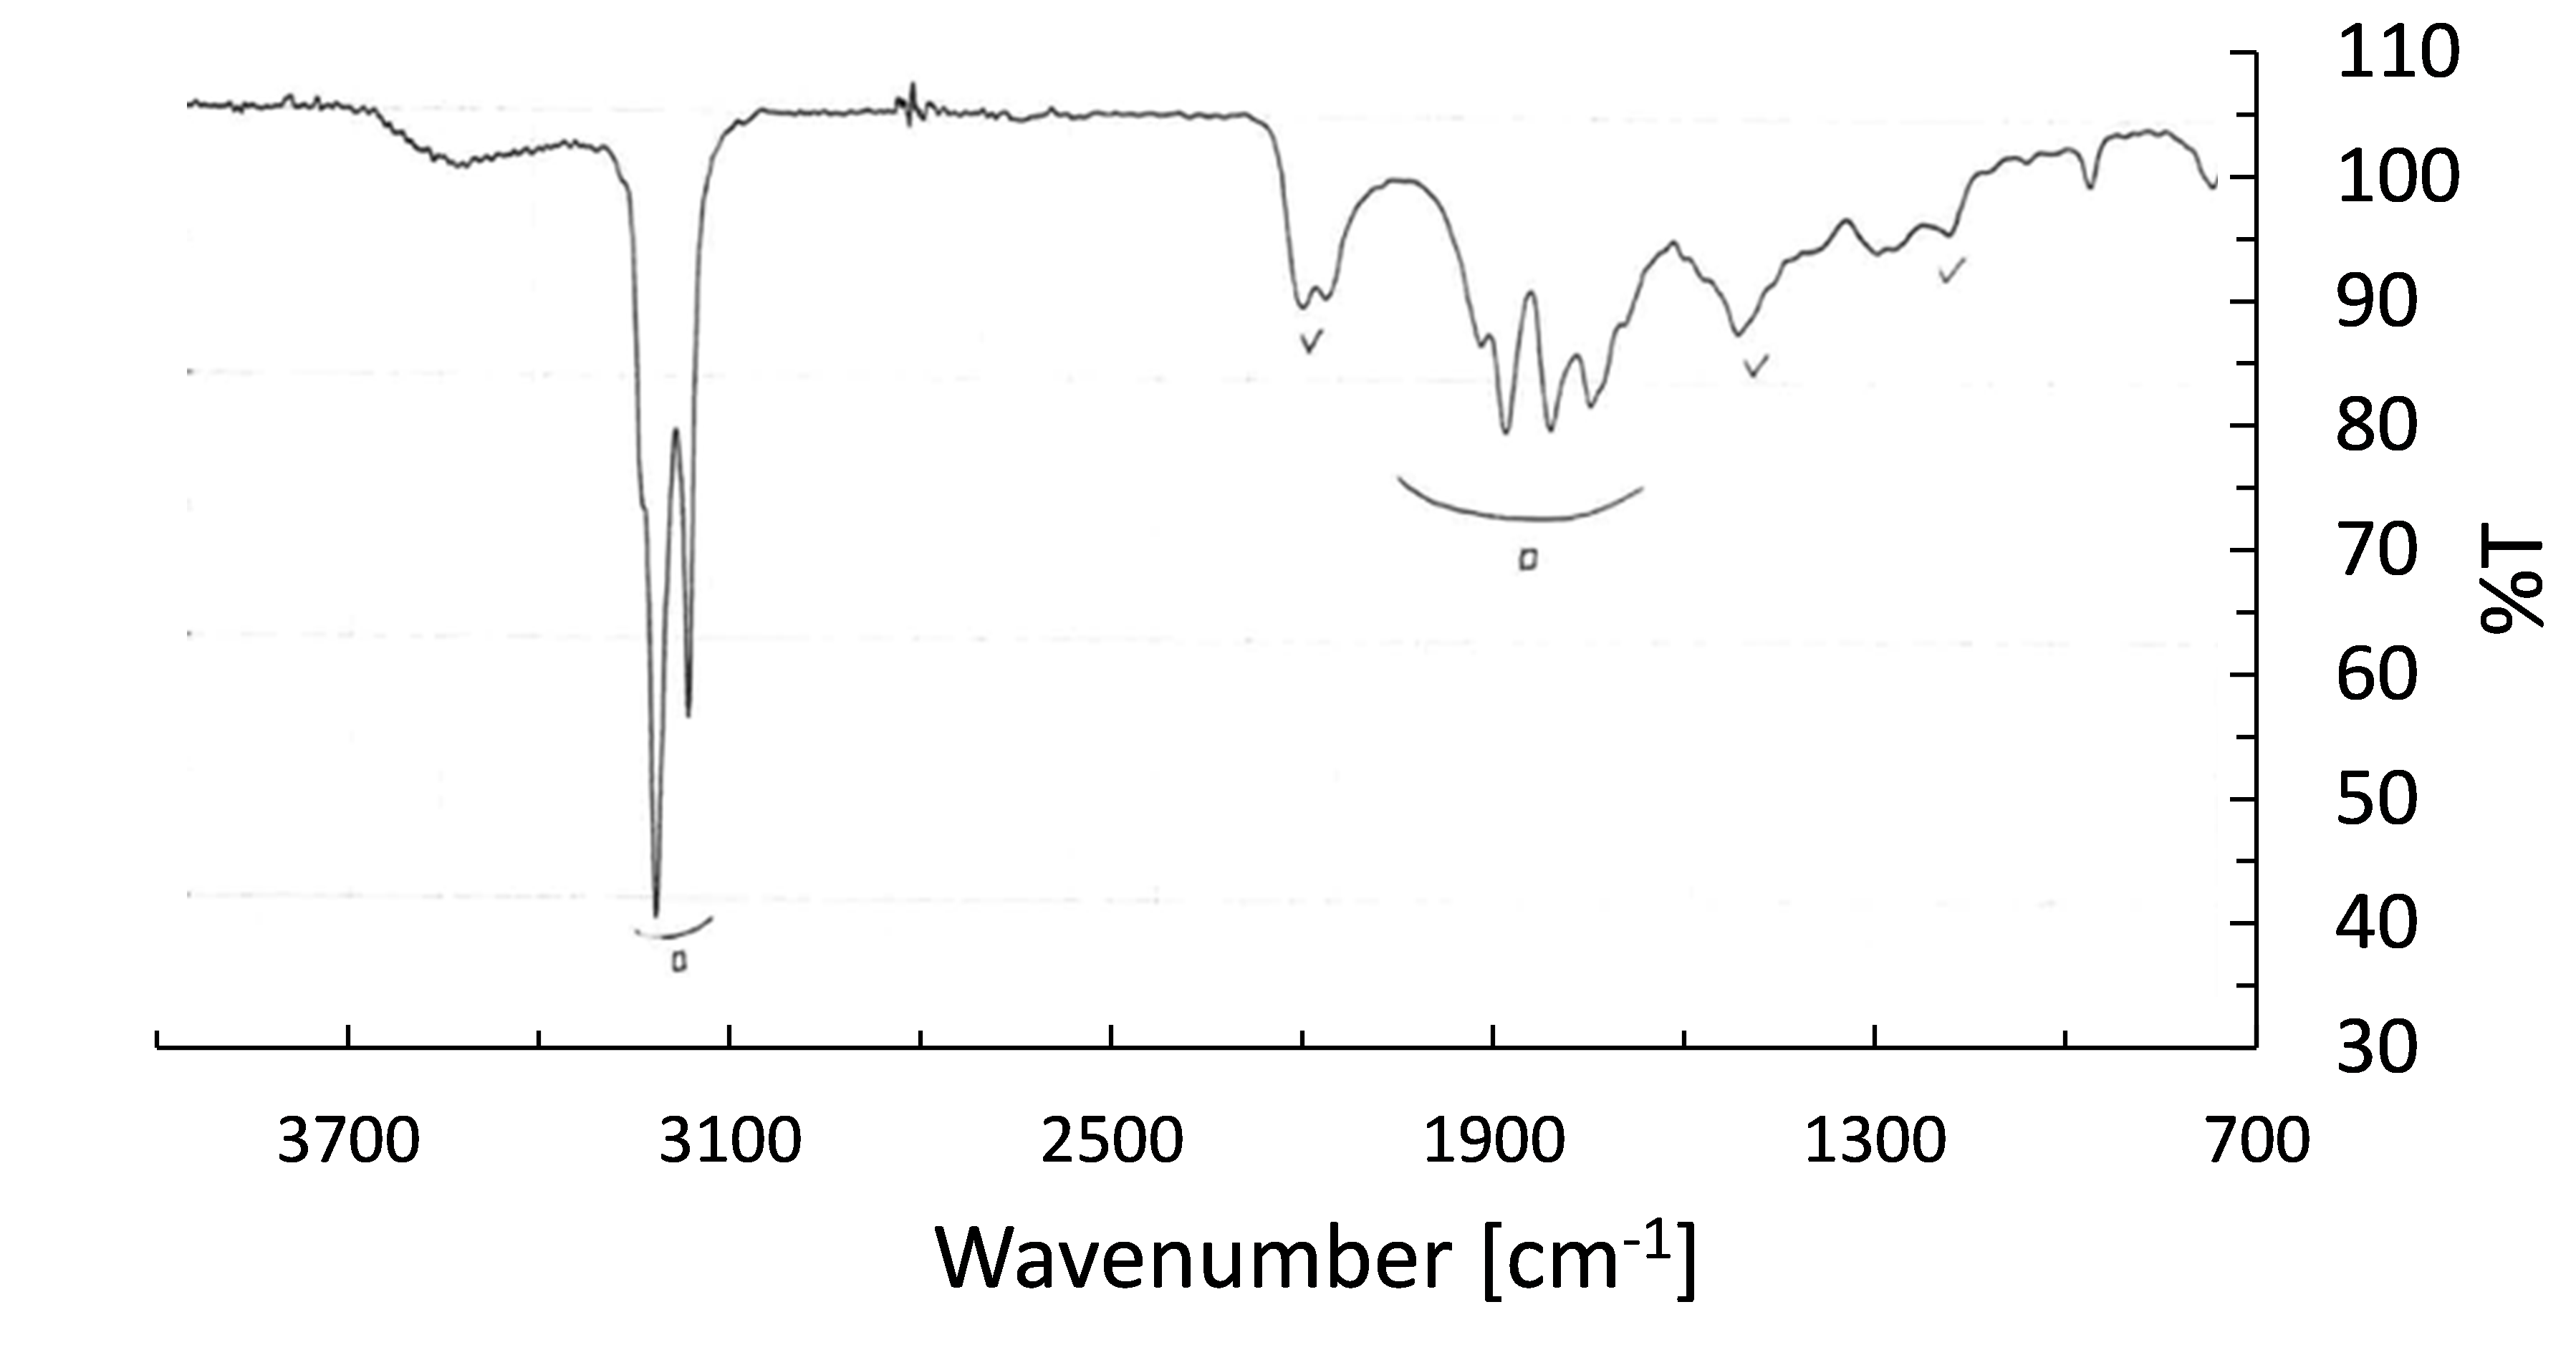
\includegraphics[width=\linewidth]{imgs/ch3/fig4.png}
    \caption{FT-IR spectra of the joint surface}
    \label{ch3fig4}  
    \end{minipage}
    \begin{minipage}[t]{0.7\textwidth}
    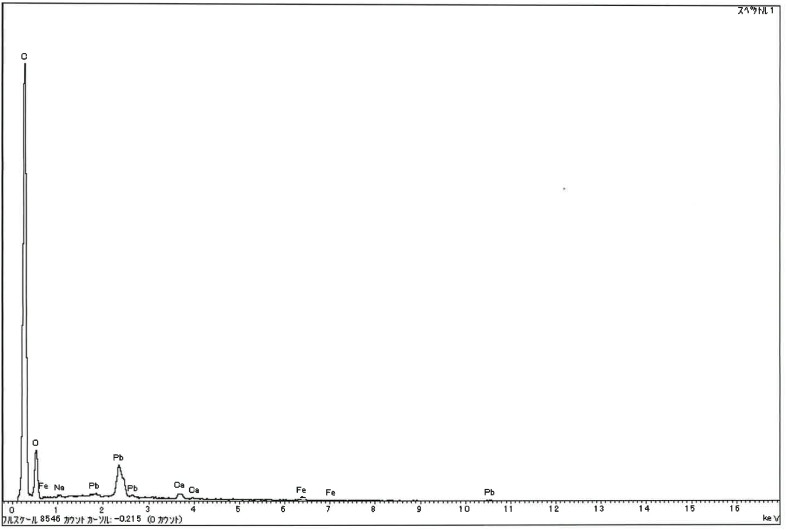
\includegraphics[width=\linewidth]{imgs/ch3/fig5.png}
    \caption{EDX-spectrum of the joint surface}
    \label{ch3fig5}  
    \end{minipage}
\end{figure}

From Fig. \ref{ch3fig5}, it can be inferred that the lead oxide on the joint surface was confirmed to exist on the joint surface, and there was also iron oxide. By means of FT-IR spectra that can confirm iron oxide is not red rust (iron(III) oxide), but a black oxide film formed when the steel is manufactured.


\subsection{Small-scale slip test}

\subsubsection{Loading and measuring methods}

Fig. \ref{ch3fig6} shows a loading machine and loading methodology, and Fig. \ref{ch3fig6a}, Fig. \ref{ch3fig6b} shows the general diagram and the detailed diagram, respectively. A screw-jack applies a horizontal load to two sets of specimens until it reaches the target clamping force. And they are then applying a vertical load to the specimens by a universal loading machine. There is a Displacement Transducer on each side of specimens, and they will be initialed to monitor the slip of the test specimen after the horizontal load is complete. Both horizontal and vertical loads applied were monitored by using a load cell.

\begin{figure}[htbp]
    \centering
    \begin{subfigure}[t]{0.58\textwidth}
    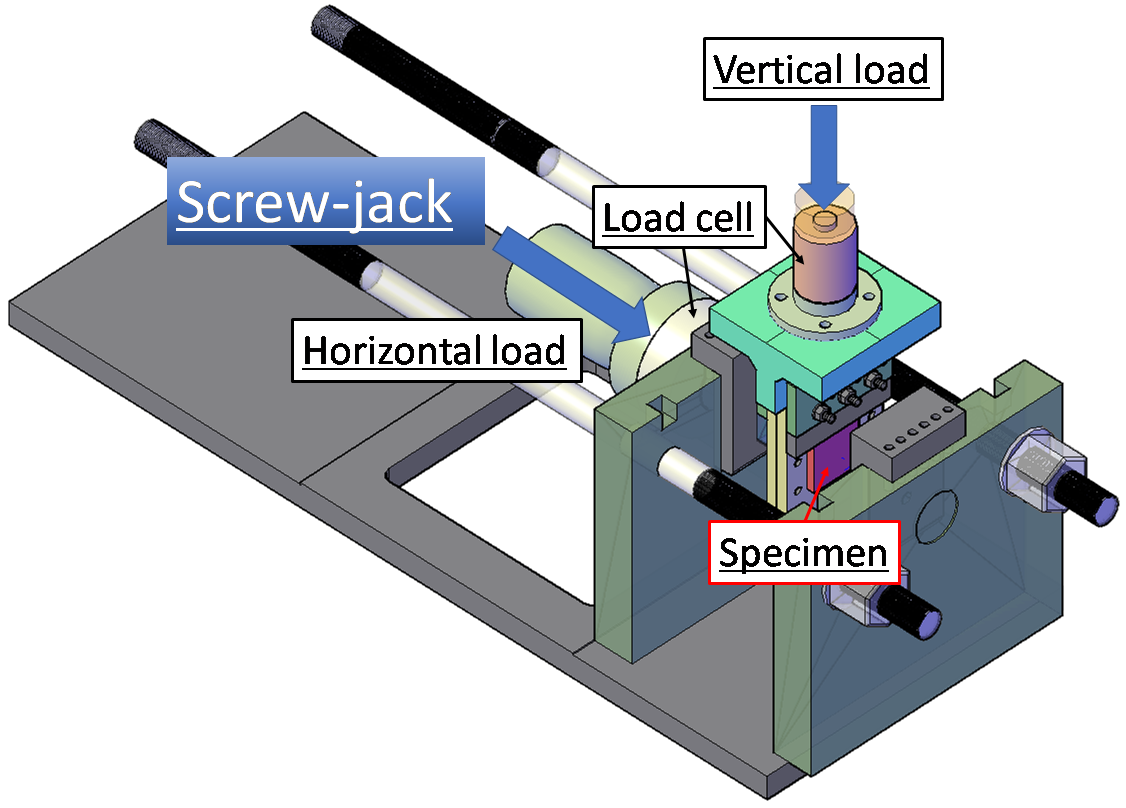
\includegraphics[width=\linewidth]{imgs/ch3/fig6a.png}
    \caption{General diagram}
    \label{ch3fig6a}  
    \end{subfigure}
    \hfill
    \begin{subfigure}[t]{0.38\textwidth}
    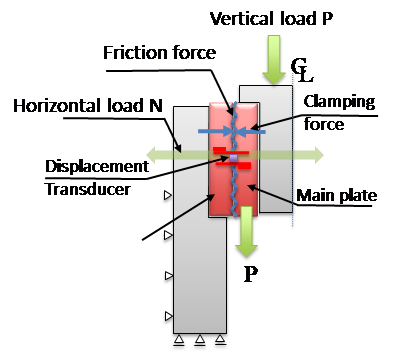
\includegraphics[width=\linewidth]{imgs/ch3/fig6b.png}
    \caption{Detailed diagram}
    \label{ch3fig6b}  
    \end{subfigure}
    \caption{Test setup}
    \label{ch3fig6}
\end{figure}

The universal loading machine will be loading on 0.5 kN/s until a slip occurred. Then, the slip coefficient is calculated by the relationship between the vertical load and displacement.

\subsubsection{Specimens}

A total of 48 set specimens are cut out from the same riveted bridge's joint. The position of cut out and the size of specimens as shown in Figure 7a, and b respectively. In order to explore the influence of the clamping force on the slip coefficient, the specimens are divided into three groups according to the different clamping forces introduced. The three groups of specimens are 24 sets of 100\% standard clamping forces, 12 sets of 75\%, and 50\% standard clamping forces $N$. 

\begin{figure}[htbp]
    \centering
    \begin{subfigure}[t]{0.48\textwidth}
    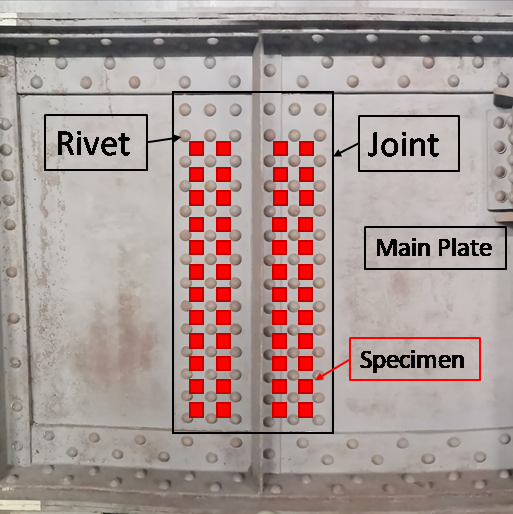
\includegraphics[width=\linewidth]{imgs/ch3/fig7a.png}
    \caption{Cross-beam}
    \label{ch3fig7a}  
    \end{subfigure}
    \hfill
    \begin{subfigure}[t]{0.48\textwidth}
    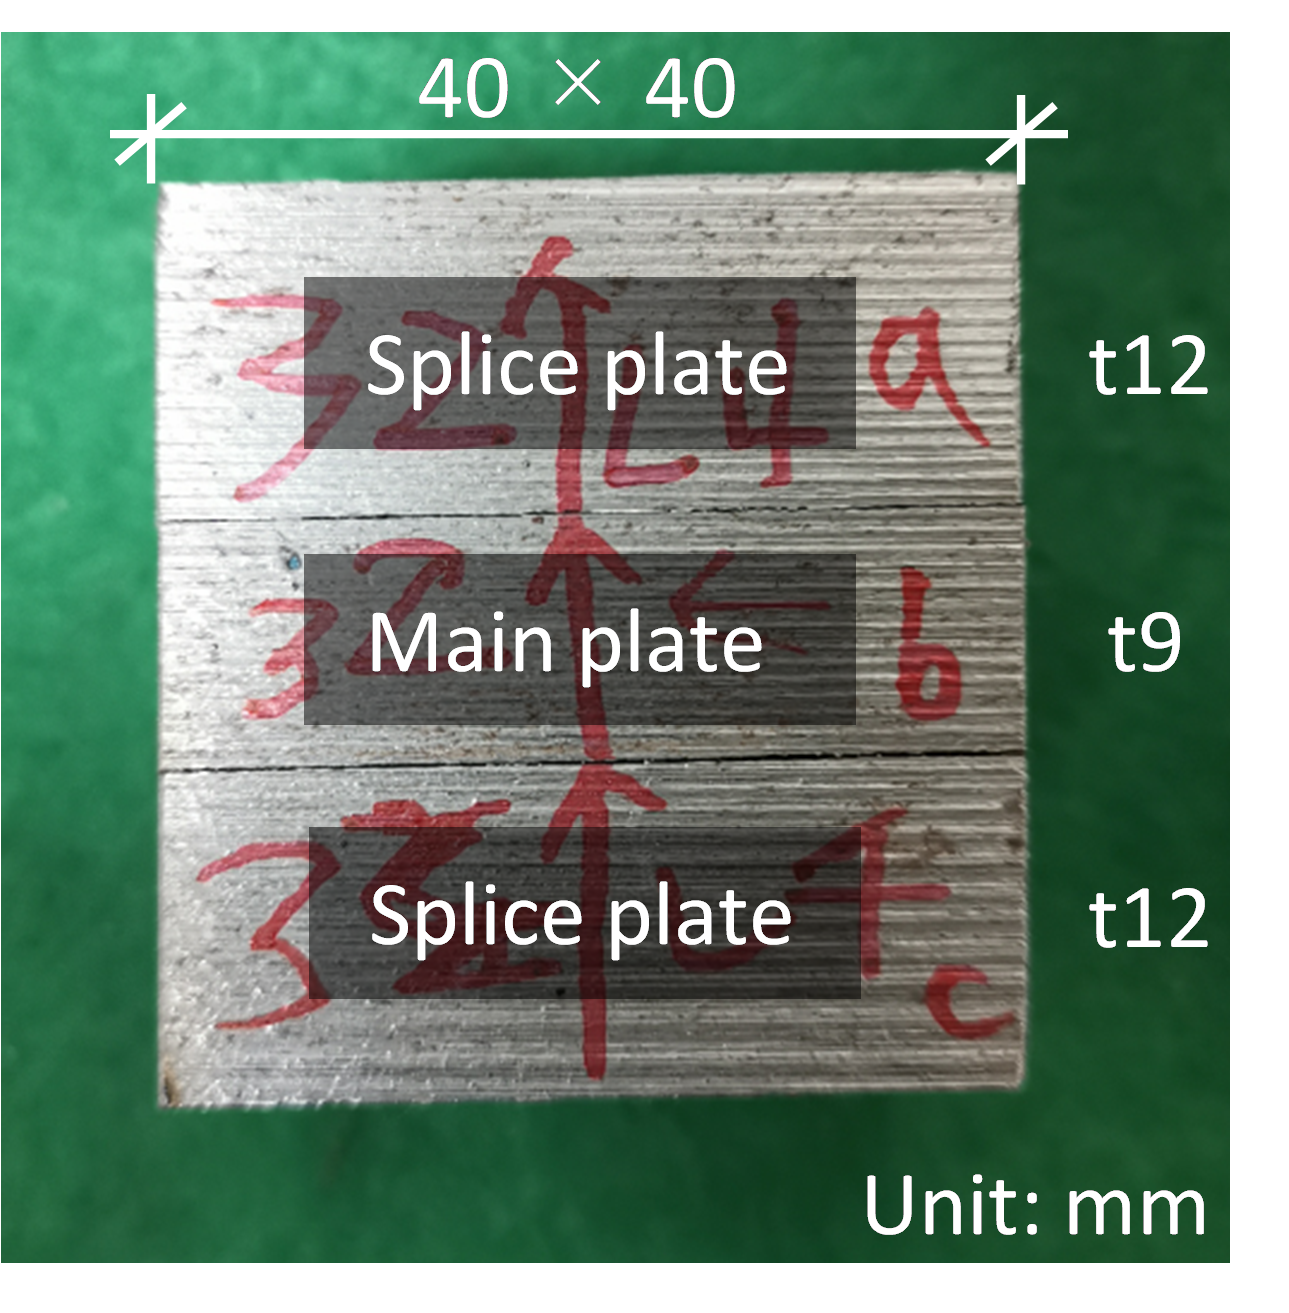
\includegraphics[width=\linewidth]{imgs/ch3/fig7b.png}
    \caption{Specimens section}
    \label{ch3fig7b}  
    \end{subfigure}
    \caption{Specimens' cut out location and size}
\end{figure}

The standard clamping force is calculated by multiplying the standard bolt contact pressure by the contact area. The assumed contact pressure area was calculated as the contact pressure distributed at 45° \cite{rotscher1927maschinenelemente}, as shown in Fig. \ref{ch3fig8}. When the splice plate's thickness is 12 mm, the standard bolt contact pressure can be calculated as 64.9 N/mm2. Here it is assumed that the bolt is the most commonly used F10T-M22 in Japanese bridges.


\begin{figure}[htbp]
\centering
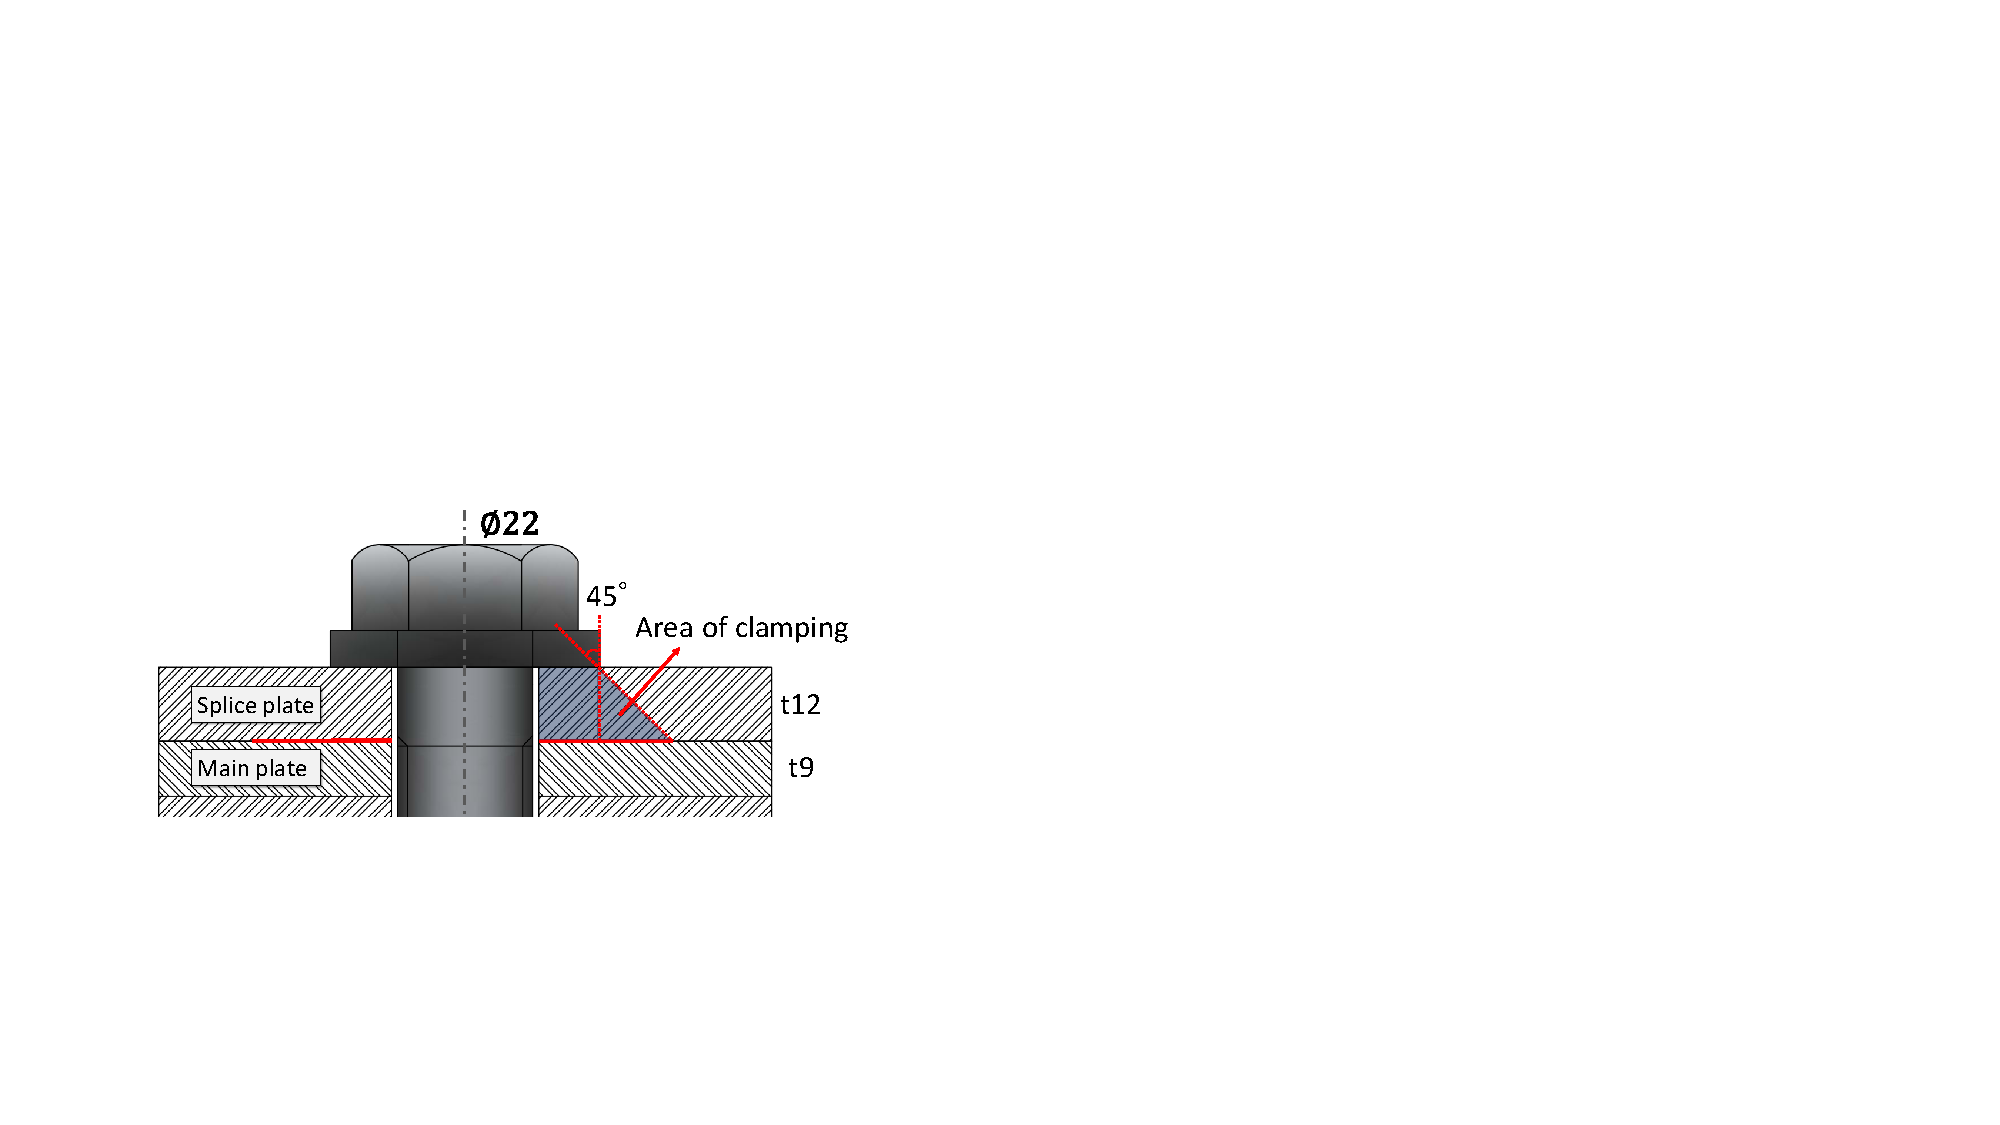
\includegraphics[width=0.65\linewidth]{imgs/ch3/fig8.pdf}
\caption{Definition of clamping area (unit: mm)}
\label{ch3fig8}  
\end{figure}

For example, for the M22 size bolt, the euivalent contact area $A_{ct-m22}$ is:
\begin{equation*}
    A_{ct-m22} = \pi (r_h-r_b)^2
\end{equation*}

Where, the  bolt shank radius $r_b$ is 11 mm, bolt hole radius $r_h$ is 11.75 mm.
the equivalent contact pressure $\sigma_{ct-m22}$ is:
\begin{equation*}
    \sigma_{ct-m22} = \frac{N}{A_{M22}} = 64.9 Mpa
\end{equation*}

Where, $N$ is the bolt standard preload, M22-F10T bolt is 205 kN.
The applied horizontal force (Converted preload) $N_{cp}$ is 
\begin{equation*}
    N_{cp} = \sigma_{ct-m22} \times A_{cts} =64.9 \times 40 \times 40 = 103.8 kN
\end{equation*}
Where, $A_{cts}$ is specimens size for small-scale slip test


\subsubsection{Test result}

The test results are summarized in Table \ref{ch3tab1}. The table summarizes the slip coefficients and their variation of all the specimens with 100\%, 75\%, and 50\% of standard clamping force.

\begin{table}[htbp]
\centering
\caption{Summary of the slip coefficient and estimation of variability}
\label{ch3tab1}
\scalebox{0.95}{
\begin{tabular}{@{}cccccccc@{}}
\toprule
\multirow{3}{*}{Specimens} &
  \multicolumn{3}{c}{Slip coefficient} &
  \multirow{3}{*}{\begin{tabular}[c]{@{}c@{}}Standard \\ Deviation \\ (SD, $\sigma$) \end{tabular}} &
  \multirow{3}{*}{\begin{tabular}[c]{@{}c@{}}Standard \\ Error \\ (SE) \end{tabular}} &
  \multirow{3}{*}{\begin{tabular}[c]{@{}c@{}}Coefficient \\ of Variation \\ (C.V.) \end{tabular}} &
  \multirow{3}{*}{\begin{tabular}[c]{@{}c@{}}The \\ Number \\ of data \end{tabular}} \\ \cmidrule(lr){2-4}
        & \multirow{2}{*}{Average} & \multirow{2}{*}{Max}   & \multirow{2}{*}{Min}   &        &        &        &    \\
        &   &     &     &        &        &        &    \\ \midrule
All     & 0.274   & 0.386 & 0.173 & 0.0525 & 0.0076 & 0.1917 & 48 \\
100\%CF & 0.291   & 0.386 & 0.192 & 0.0491 & 0.0100 & 0.1688 & 24 \\
75\%CF  & 0.240   & 0.341 & 0.173 & 0.0482 & 0.0139 & 0.2009 & 12 \\
50\%CF  & 0.274   & 0.351 & 0.208 & 0.0504 & 0.0145 & 0.1839 & 12 \\ \bottomrule
\end{tabular}}
\end{table}

The average slip coefficient is 0.274, the coefficient of variation is 0.19, and the -2σ is 0.169. It can be found that the degree of dispersion of the slip coefficient is not low. Furthermore, it could be concluded that the slip coefficient from the slip test follows a normal distribution by the Shapiro-Wilk normality test \cite{shapiro1965Analysis}. The normal distribution of the slip coefficient is shown in Fig. \ref{ch3fig10}. The 95\% confidence interval is presented as the arithmetic mean ± 1.96 SE (Standard Error) (0.259--0.289).

\begin{figure}[htbp]
    \centering
    \begin{subfigure}[t]{0.48\textwidth}
    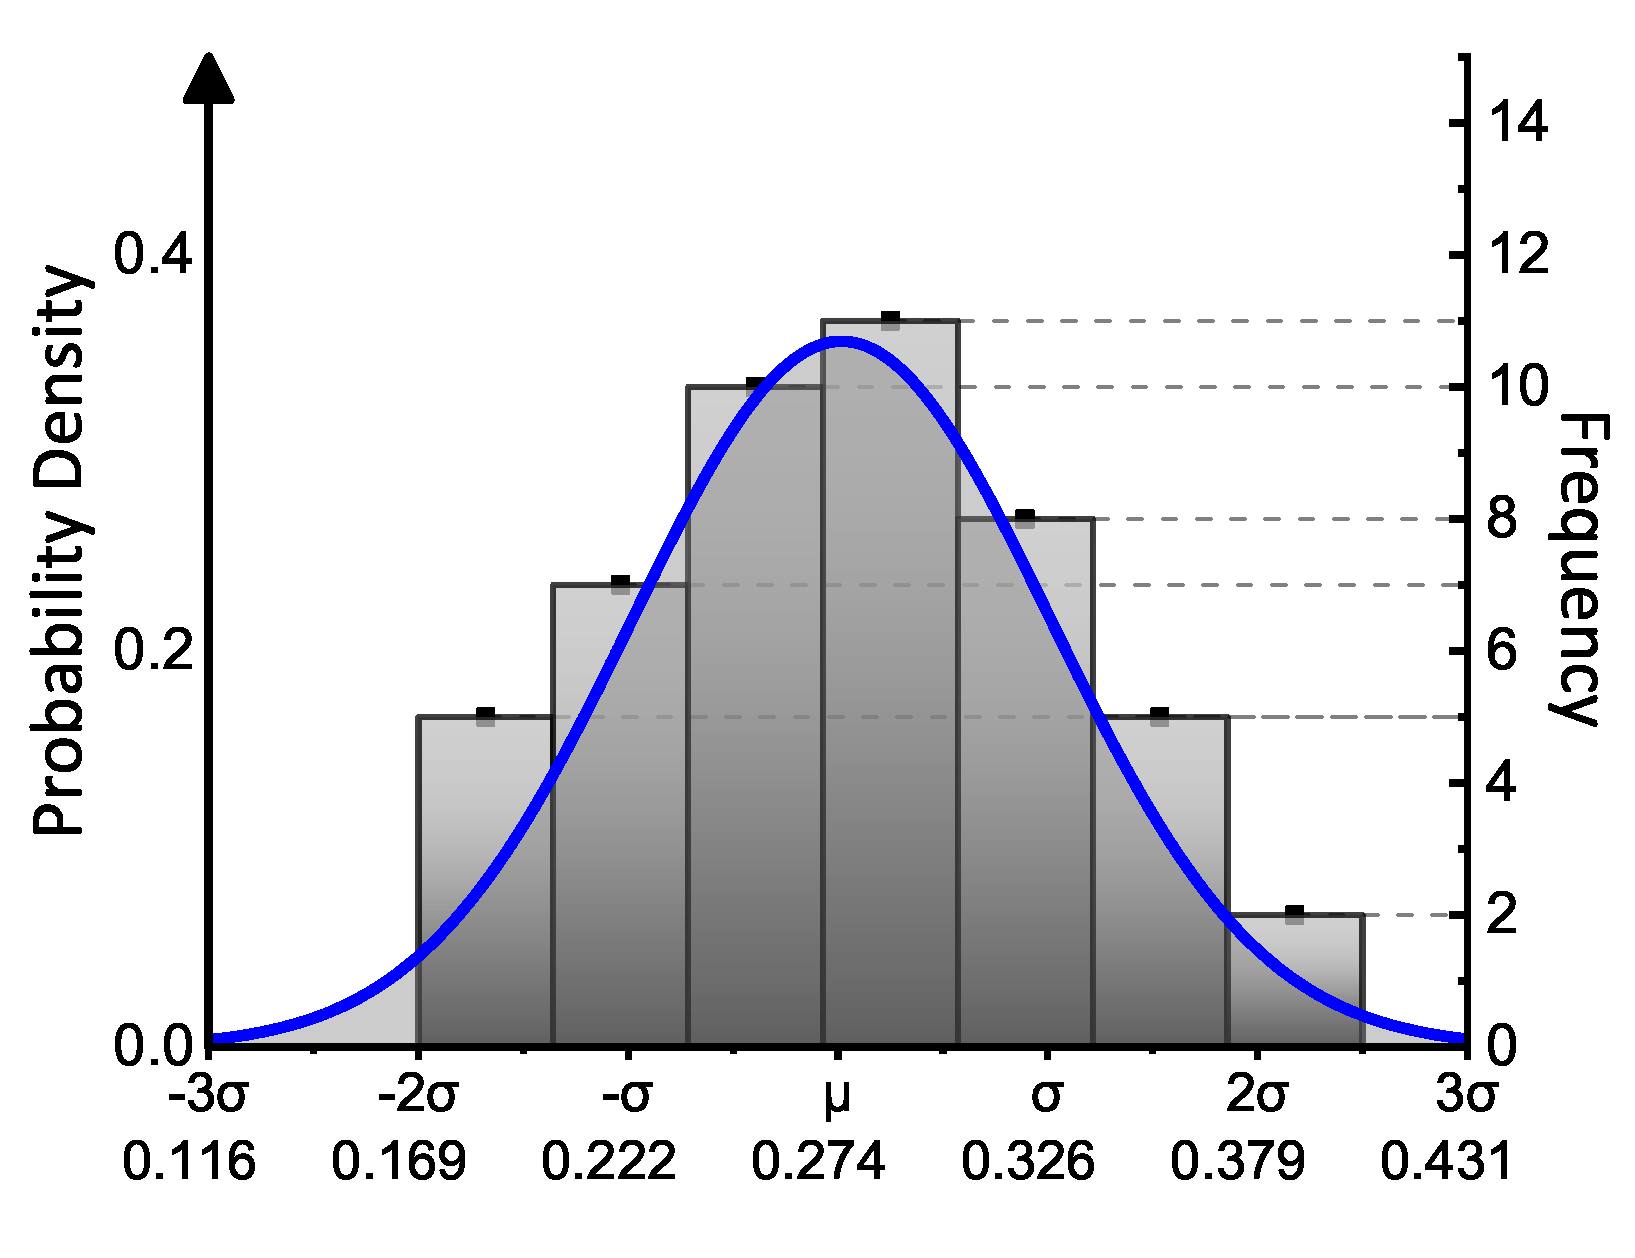
\includegraphics[width=\linewidth]{imgs/ch3/fig10a.eps}
    \caption{Normal distribution}
    \label{ch3fig10a}  
    \end{subfigure}
    \hfill
    \begin{subfigure}[t]{0.48\textwidth}
    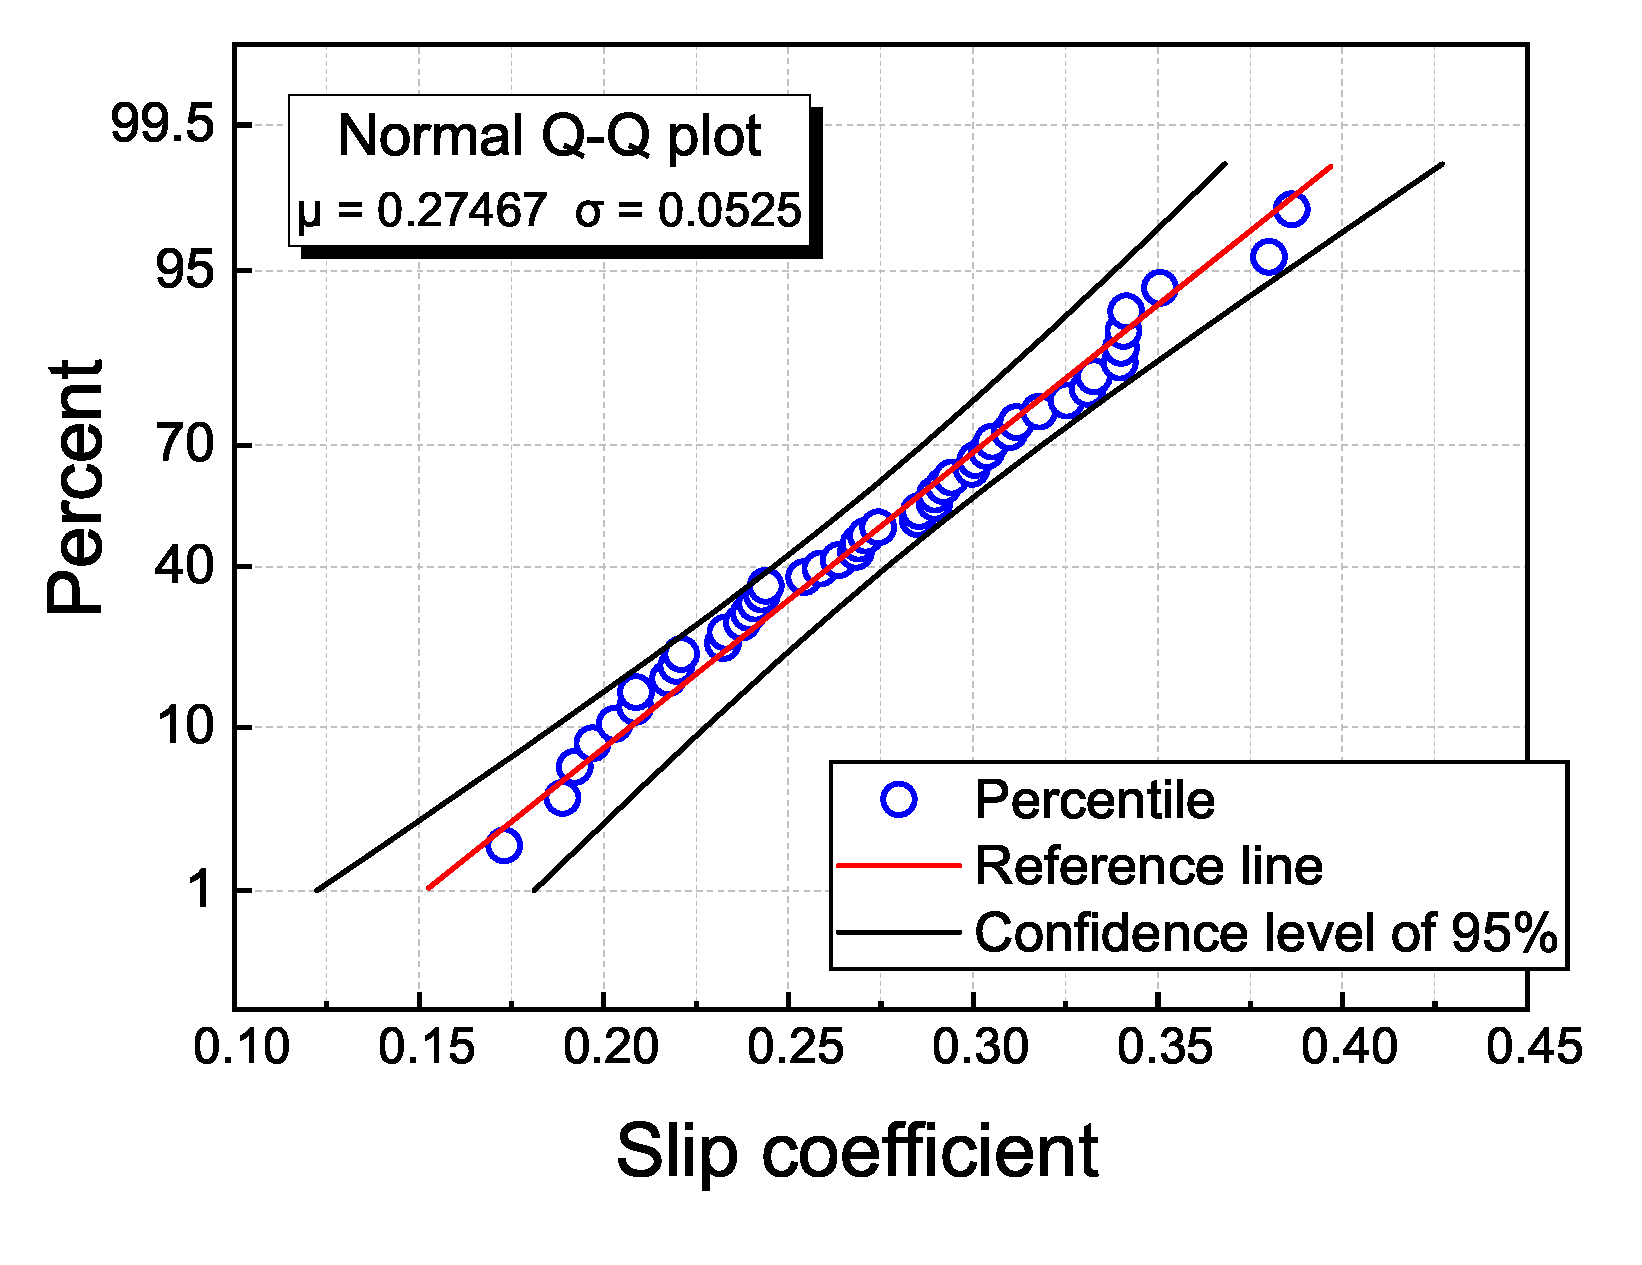
\includegraphics[width=\linewidth]{imgs/ch3/fig10b.eps}
    \caption{Q-Q plot}
    \label{ch3fig10b}  
    \end{subfigure}
    \caption{Slip coefficient distribution}
    \label{ch3fig10} 
\end{figure}

Besides, when the riveted joint surface is red lead paint, replacing the rivet with a high-strength bolt, the expected slip coefficient is 0.25-0.28 by Railway technical research institute in Japan \cite{rtri1992Manual}. However, in this experiment, it can be calculated that there is a 36\% probability that the slip coefficient is below 0.25. 

The specimens' size could cause this, and the red lead distribution is uneven, resulting in a very low slip coefficient accrued in some specimens.

The relationship between the slip coefficient and the clamping force is shown in Fig. \ref{ch3fig11}. It can be observed from the figure that the degree of dispersion of the slip coefficient has no obvious relationship with the change of clamping force; also, it can be calculated that the correlation coefficient between clamping force and slip coefficient is 0.21. On the other hand, the relationship between the slip load and clamping force is shown in Fig. \ref{ch3fig12}. As the clamping force increases, the slip load also increases.

\begin{figure}[htbp]
\centering
\begin{minipage}[t]{0.48\textwidth}
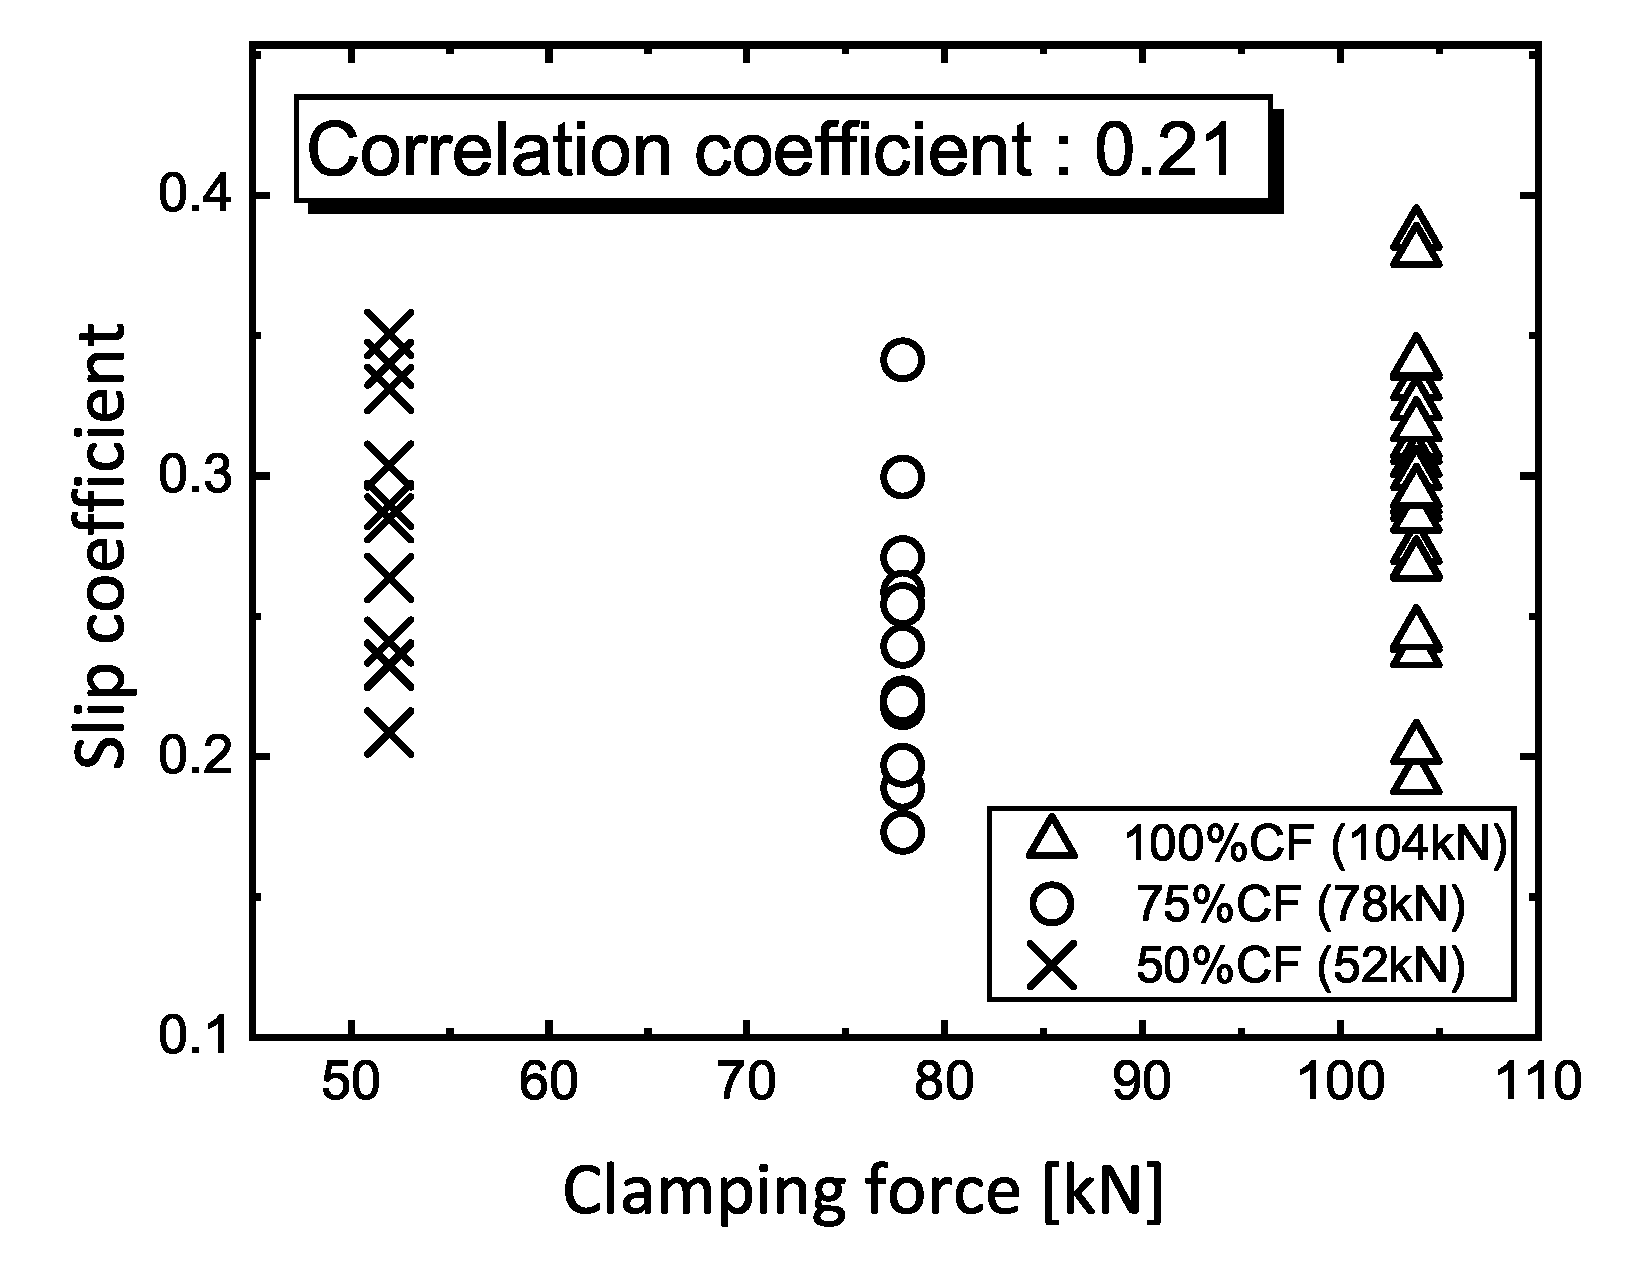
\includegraphics[width=\linewidth]{imgs/ch3/fig11.eps}
\caption{The relationship between the slip coefficient and the clamping force.}
\label{ch3fig11}
\end{minipage}
\begin{minipage}[t]{0.48\textwidth}
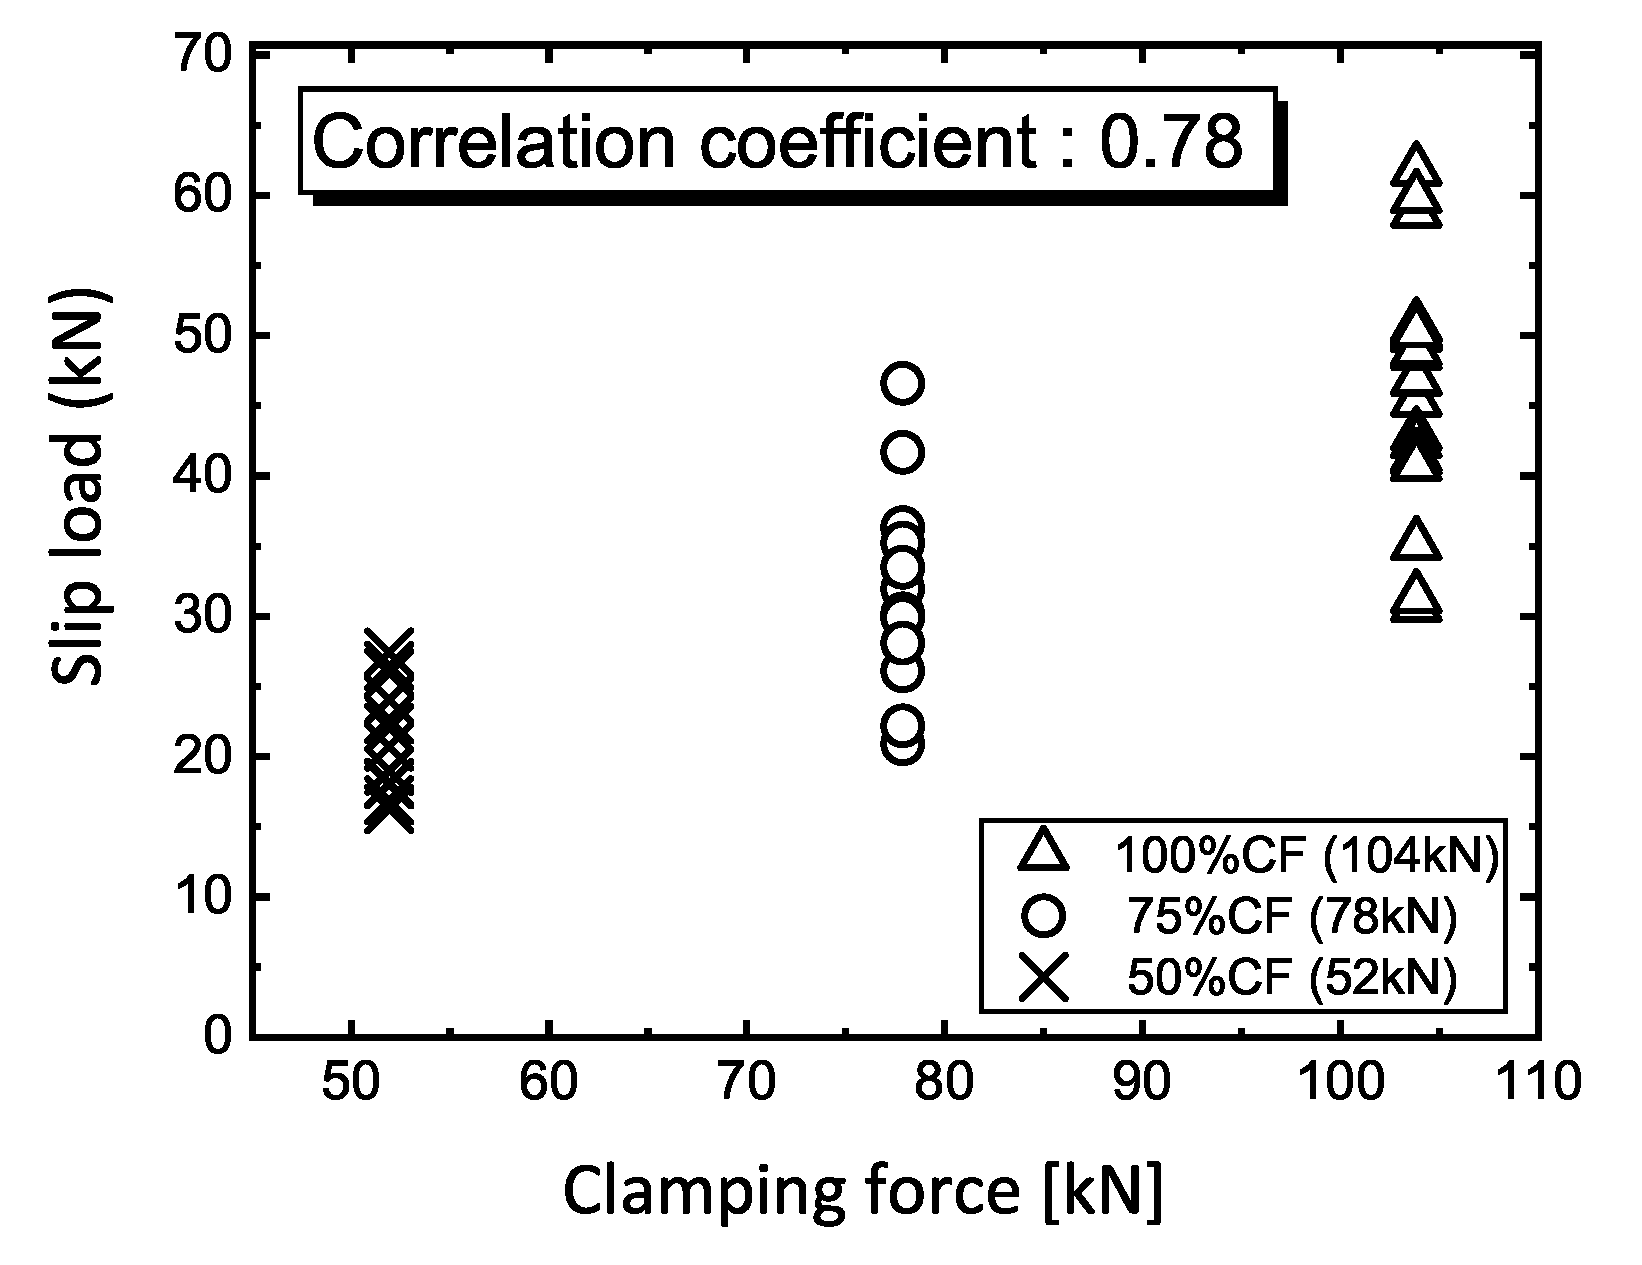
\includegraphics[width=\linewidth]{imgs/ch3/fig12.eps}
\caption{The relationship between the slip load and the clamping force.}
\label{ch3fig12}
\end{minipage}
\end{figure}

In addition, the average friction coefficient obtained is 0.295, which is 0.02 larger than the average slip coefficient of 0.274. The friction coefficient is calculated by dividing the load by the clamping force, which is taken when slippage has occurred. 

\subsection{Contact pressure distribution test}

The observation of the joint surface in section \ref{ch3sec2-1} revealed that the red lead surface distribution of specimens was much not uniform, and the red lead distribution of each specimen was also very different. In this study, a pressure distribution test is performed to investigate the influence of red lead distribution on the contact pressure and the slip coefficient. 

\subsubsection{Measuring methods}
A pressure measurement film is put into the joint surface, and then the standard clamping force is applied to the specimen by the screw-jack. When detected pressure, the film will be colored redder as the pressure increases.

\subsubsection{Measuring result}

Eight sets of specimens are conducted with a pressure distribution test. The pressure distribution was very uneven according to the aging condition of red lead paint, and the residual condition of red lead directly reflected the pressure distribution. Fig. \ref{ch3fig13} shows the pressure test results of the specimens' joint surface with a slip coefficient of 0.284 and the joint surface's condition before/after the slip test.


\begin{figure}[htbp]
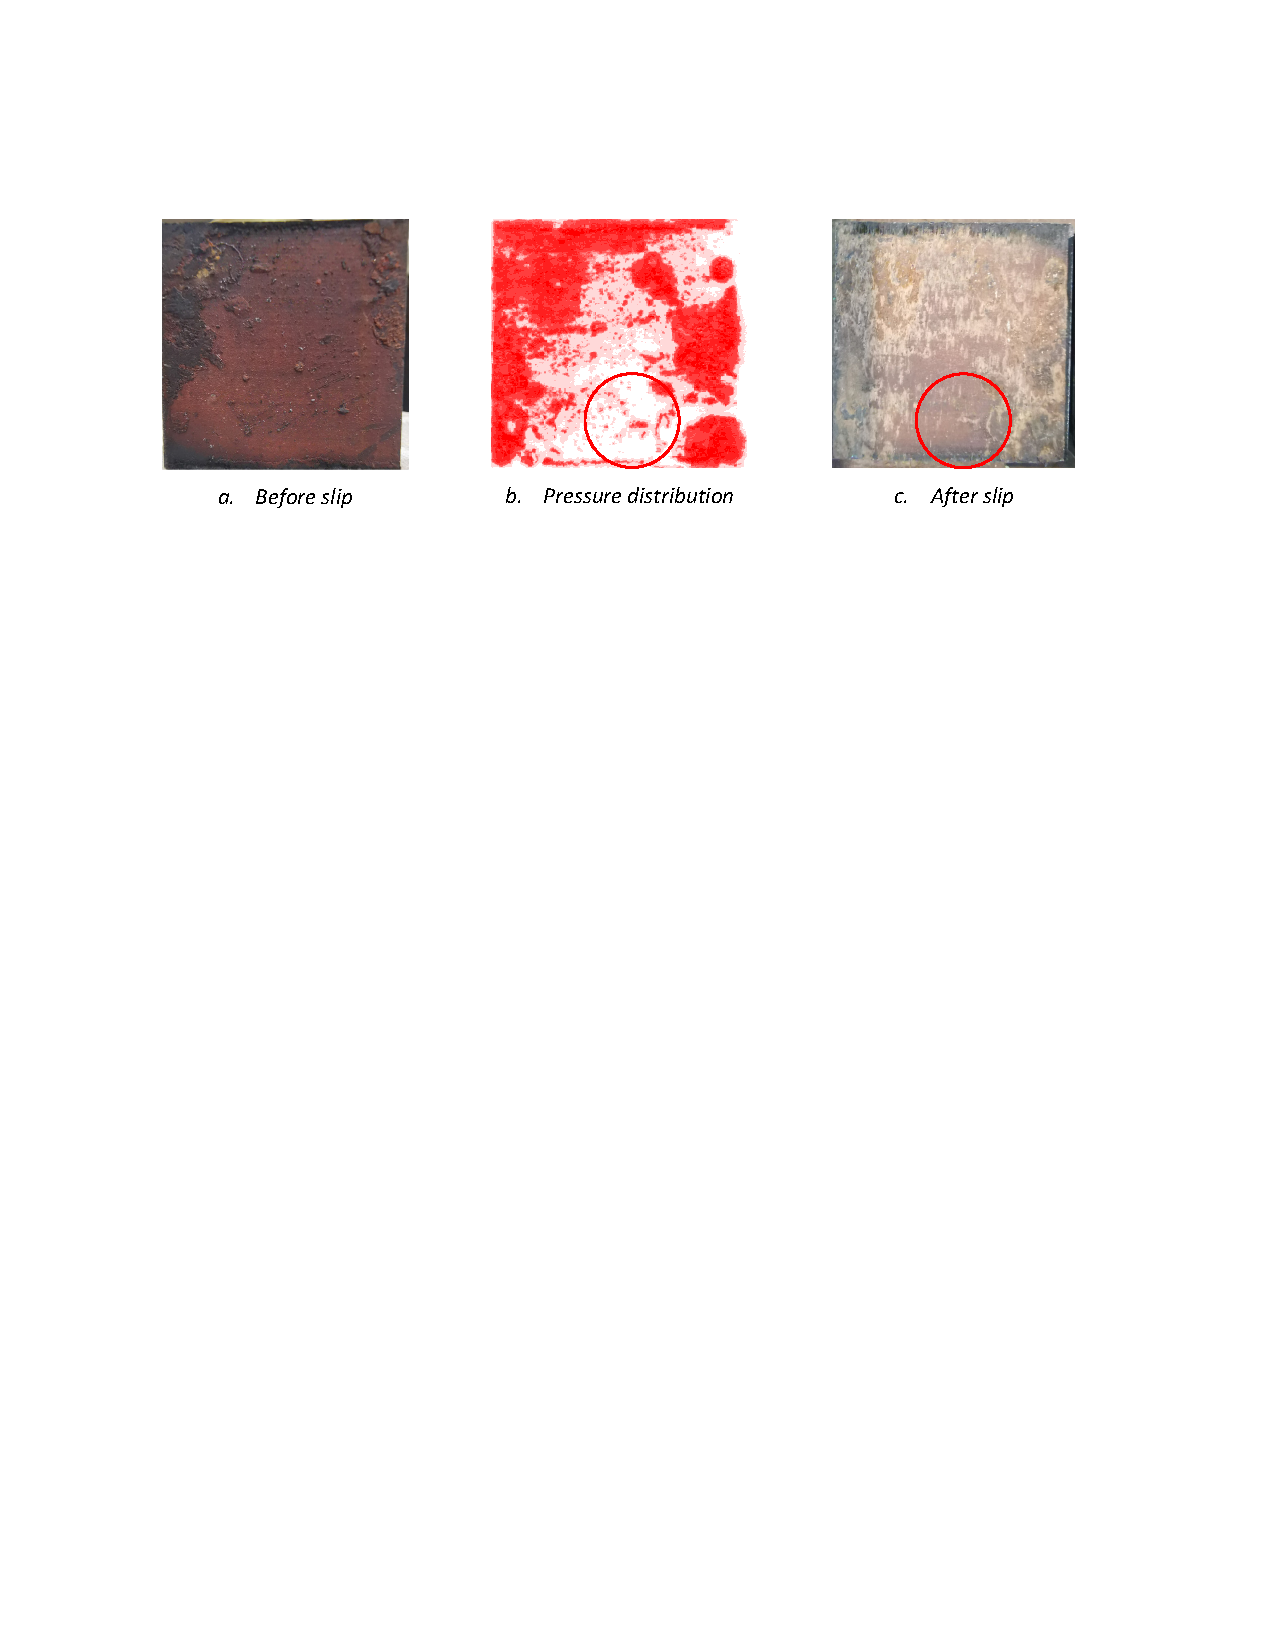
\includegraphics[width=\linewidth]{imgs/ch3/fig13.pdf}
\caption{Pressure contour figures and the condition before/after slip test.}
\label{ch3fig13}  
\end{figure}

As shown in Fig. \ref{ch3fig13}-b, the range marked with red is detected contact pressure area; the white areas have not detected contact pressure. The slip test assumes that the pressure is evenly distributed on the joint surface; however, the measuring results show that red lead paint's surface does not satisfy the average pressure distribution assumption.

As shown in Fig. \ref{ch3fig13}-c, after the slip test, the red lead paint on the joint surface was damaged. The traces of the slippage can be clearly seen. However, there are no traces of slippage near the marked red circle. The joint surface friction condition was very similar to the pressure distribution, as shown in Fig. \ref{ch3fig13}-b. It can be inferred that the white areas where no pressure is detected have no effective resistance to the friction and can be defined as the invalid contact area. On the contrary, the effective contact area is defined as where the contact pressure is detected. The effective contact pressure $σ_e$ is calculated by the effective contact area and clamping force.

\begin{equation}
    σ_e=N_0/S_e
\end{equation}
Where $N_0$ is clamping force;$ S_e$ is effective contact area. 

\begin{figure}[htbp]
\centering
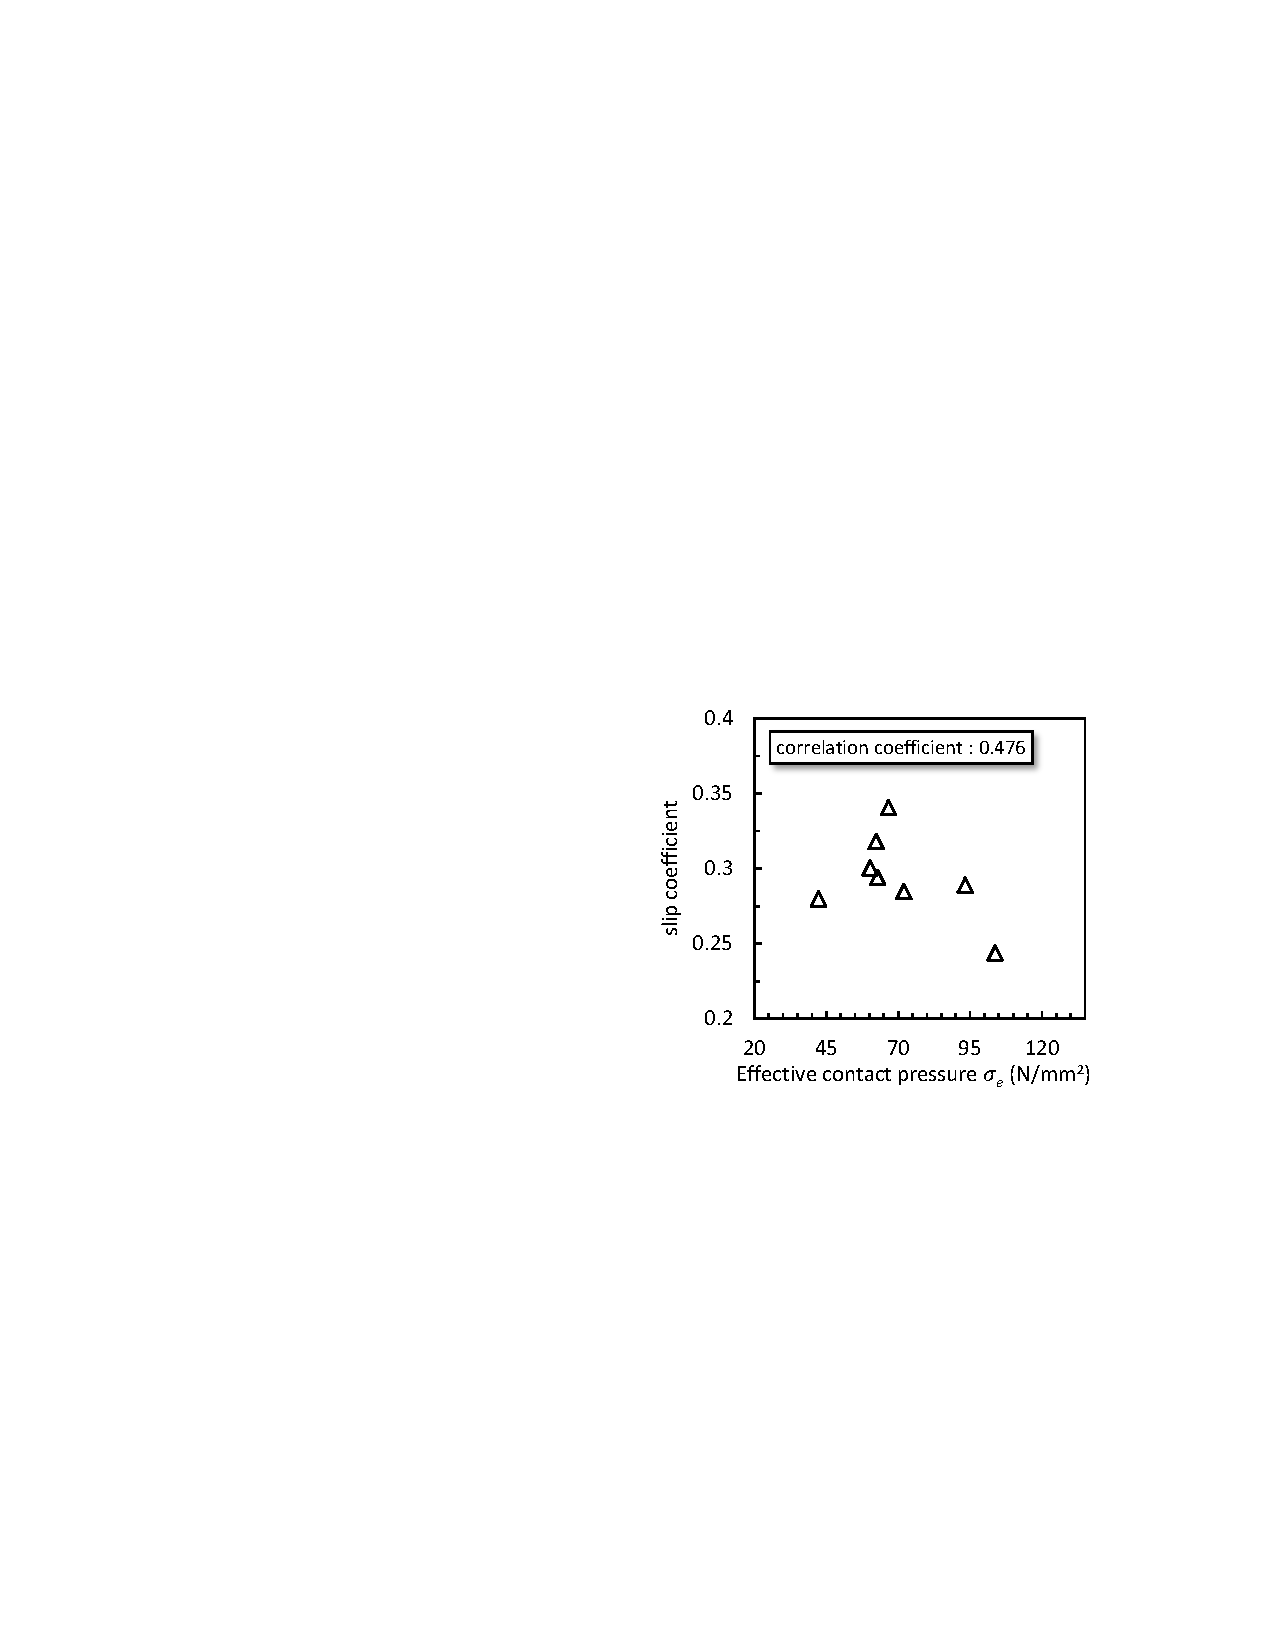
\includegraphics[width=0.65\linewidth]{imgs/ch3/fig14.pdf}
\caption{The relationship between slip coefficient and effective contact pressure}
\label{ch3fig14}  
\end{figure}

The relationship between slip coefficient and the effective contact pressure is shown in Fig. \ref{ch3fig14}. The effective contact area for each specimen is different, so although the same clamping force they have, calculated effective contact pressure is different. The correlation coefficient between the slip coefficient and the effective contact pressure is calculated as 0.476. No apparent relationship between the slip coefficient and the effective contact pressures has been observed. It could be considered that reason is the contact pressure was unevenly distributed in the effective contact area. Furthermore, the invalid pressure area and low contact pressure area do not effectively resist friction, and local slip has likely occurred. 




\section{Tensile test of partially replacement of riveted joint}

\subsection{Specimens of test}

In this study, joints part on the crossbeam(two-sided riveted joints) were sampled from the Dojima Bridge. The sampling locations and cut-off position are shown in Fig. \ref{fig-cutoff}.

\begin{figure}[htbp]
    \centering
    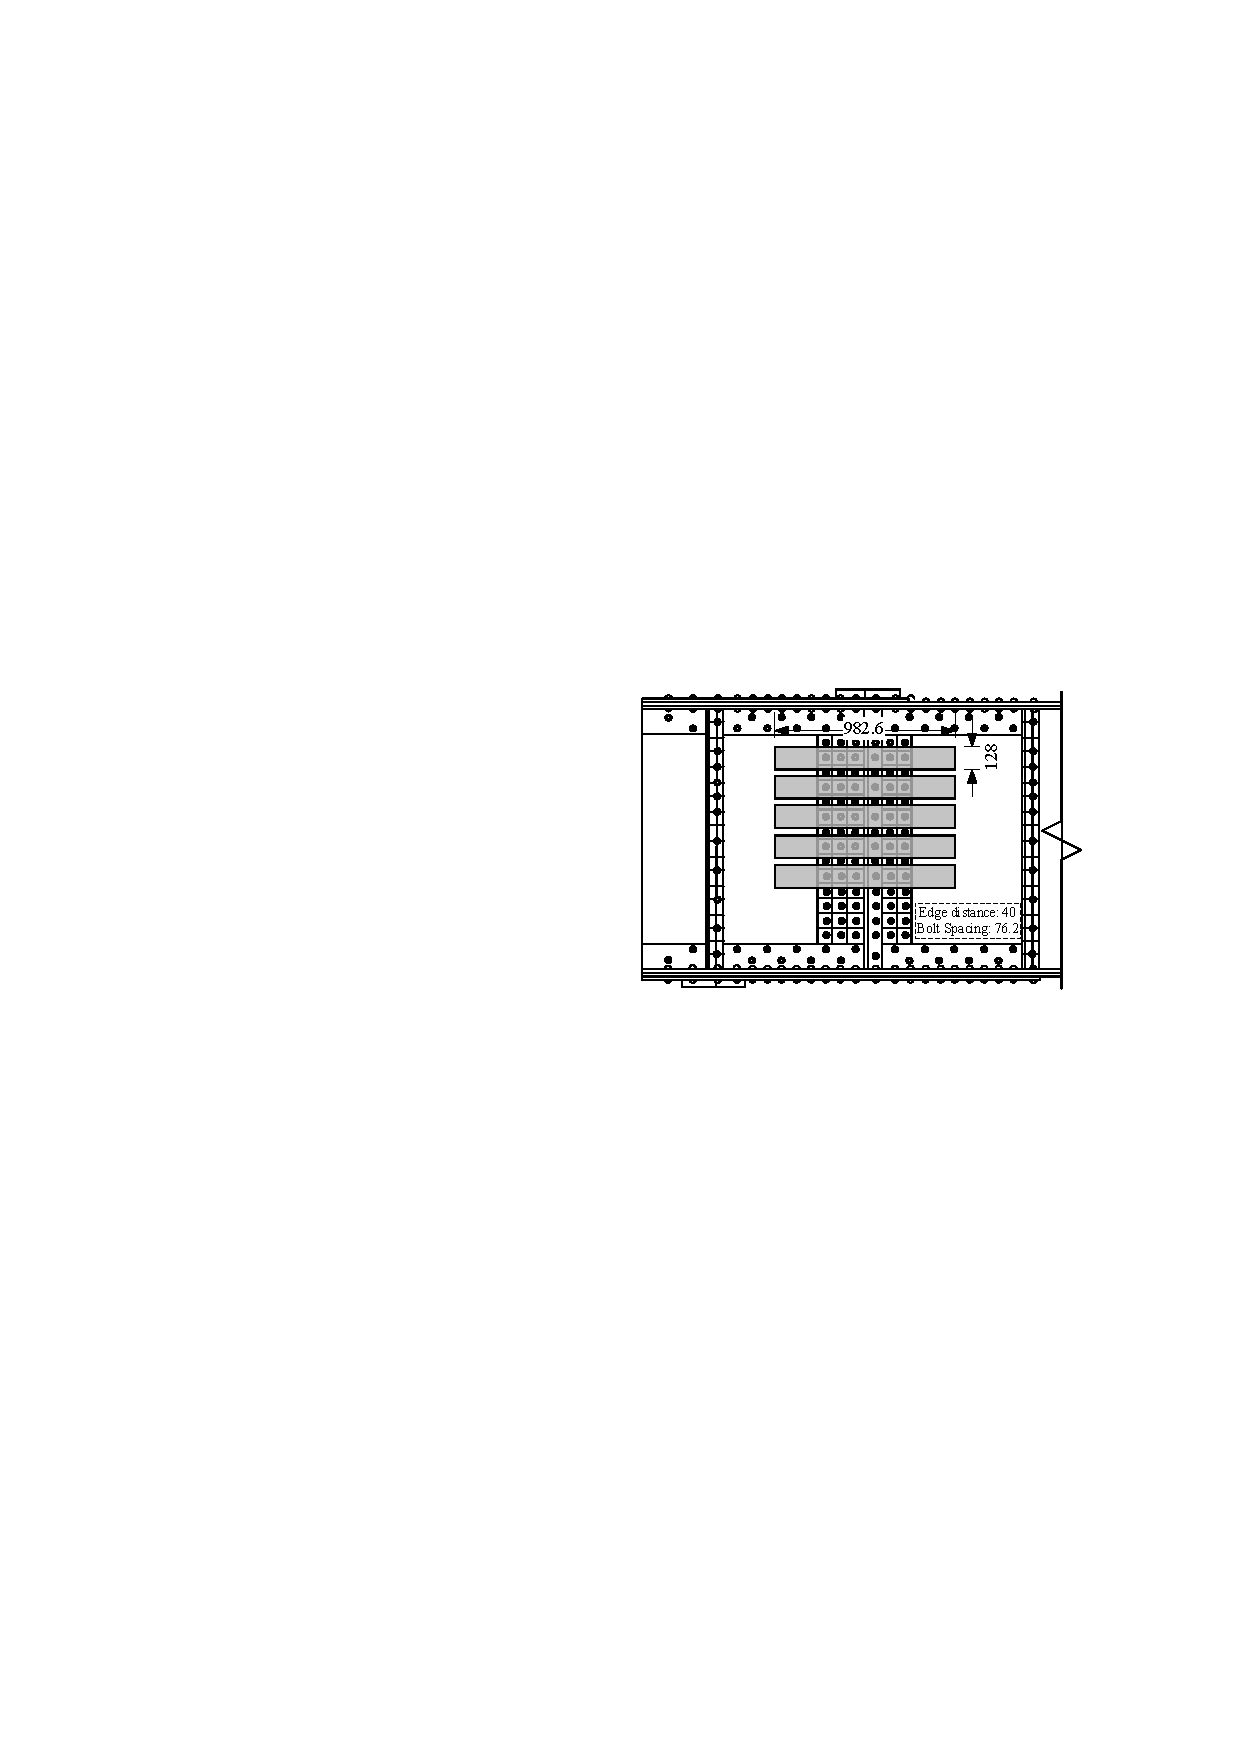
\includegraphics[width=0.6\textwidth]{imgs/ch4/figA1.pdf}
    \caption{Cut off position of each specimens}
    \label{fig-cutoff}
\end{figure}

The specimen case is shown in Fig. 3.2. The tests were carried out using a riveted joint consisting of a total of five rivets (a. riveted join case) in one row and three columns on each side as the basic case and replacing all rivets with high-strength bolts for friction joints (b. RPALL) and partially replacing rivets with high-strength bolts because in actual repair design and repair work, only corroded or fallen out rivets may be replaced with high-strength bolts. The case where rivets are partially replaced with high-strength bolts (c. RP1, d. RP2, e. RP3) is examined, as in actual repair design and repair work, only rivets that have corroded or fallen out may be replaced with high-strength bolts.

\begin{figure}[htbp]
    \centering
    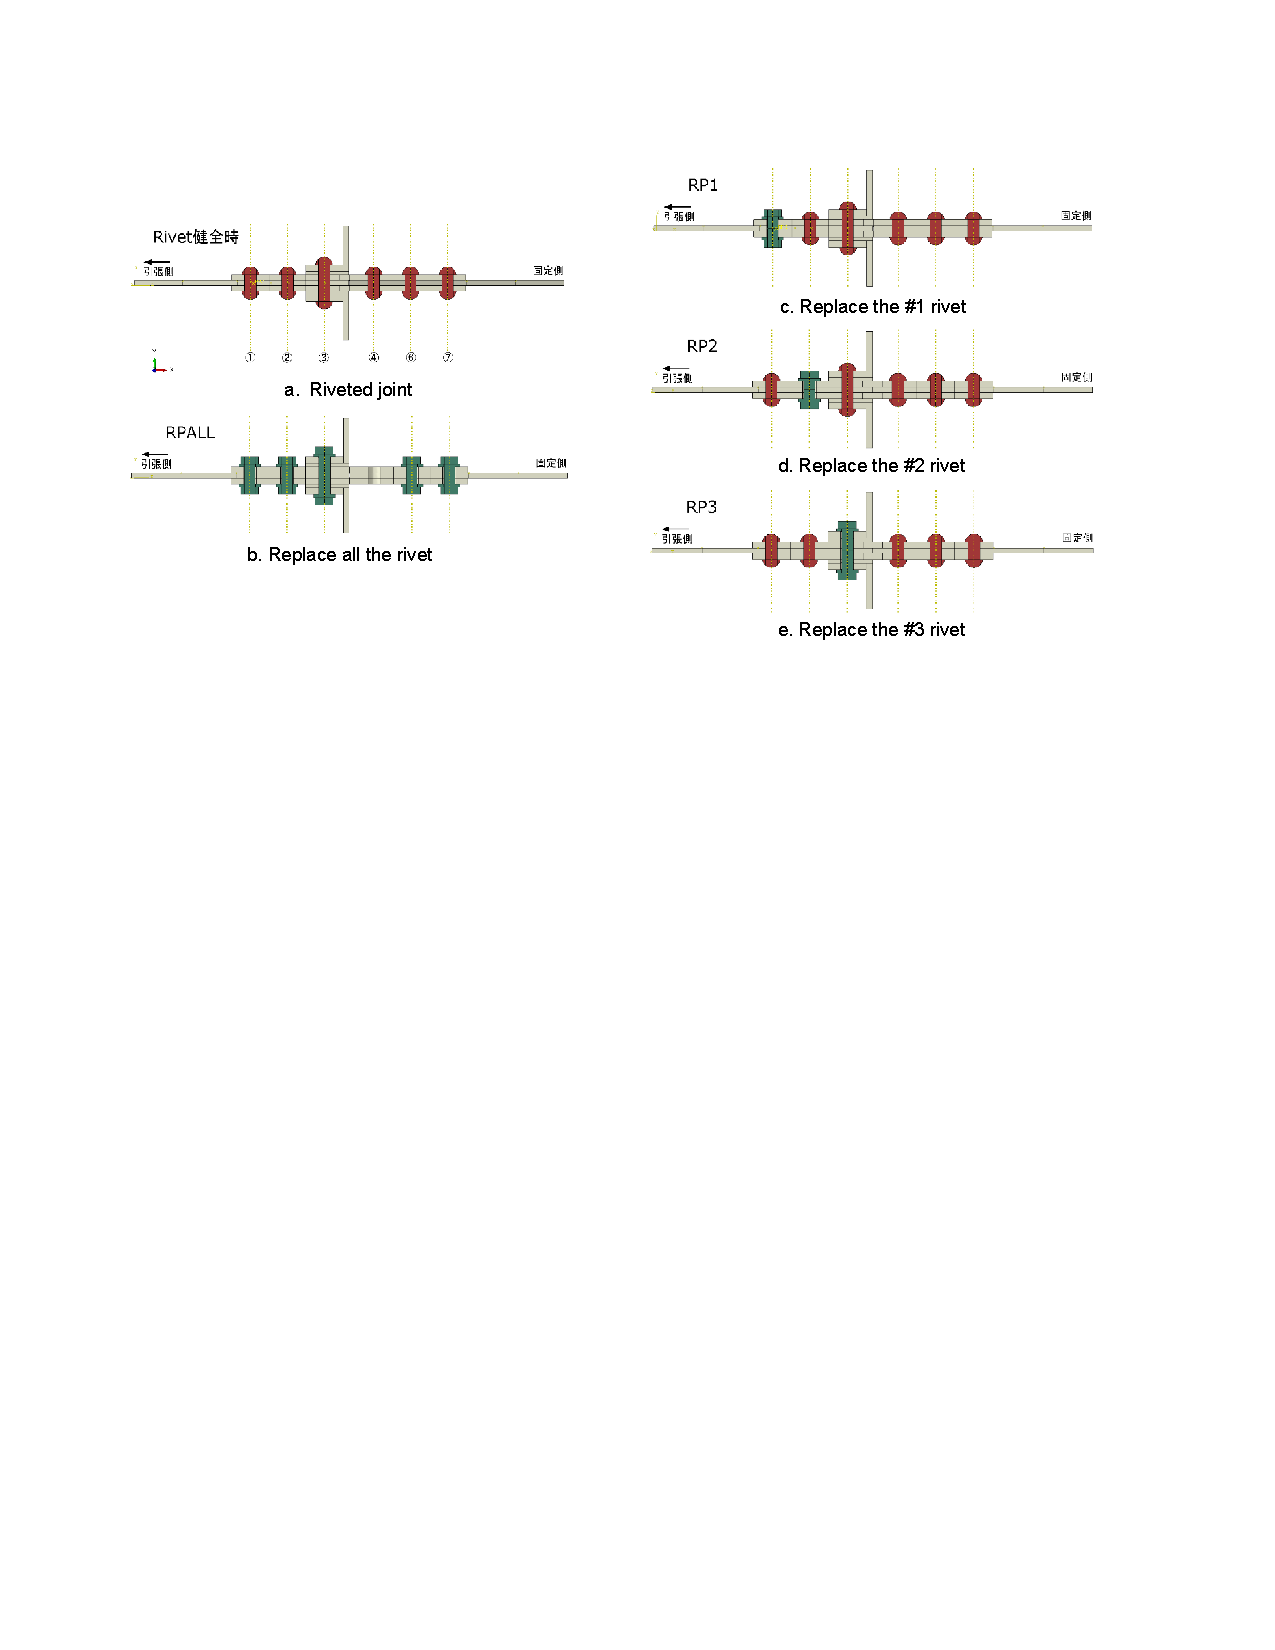
\includegraphics[width=0.8\textwidth]{imgs/ch3/riveexpcase.pdf}
    \caption{Experiment case}
    \label{fig:enter-label}
\end{figure}

Prior to the tests, specimens cut in the direction of the shaft centre were fabricated as shown in Fig. \ref{fig-ch3beasta}, the hole diameter and the gap between the rivet and the steel plate were measured and the filling status of the rivets was observed in order to ascertain the filling status of the rivets. If gaps existed, water flowed through the gaps and corrosion damage was also observed.

\begin{figure}[htbp]
    \centering
    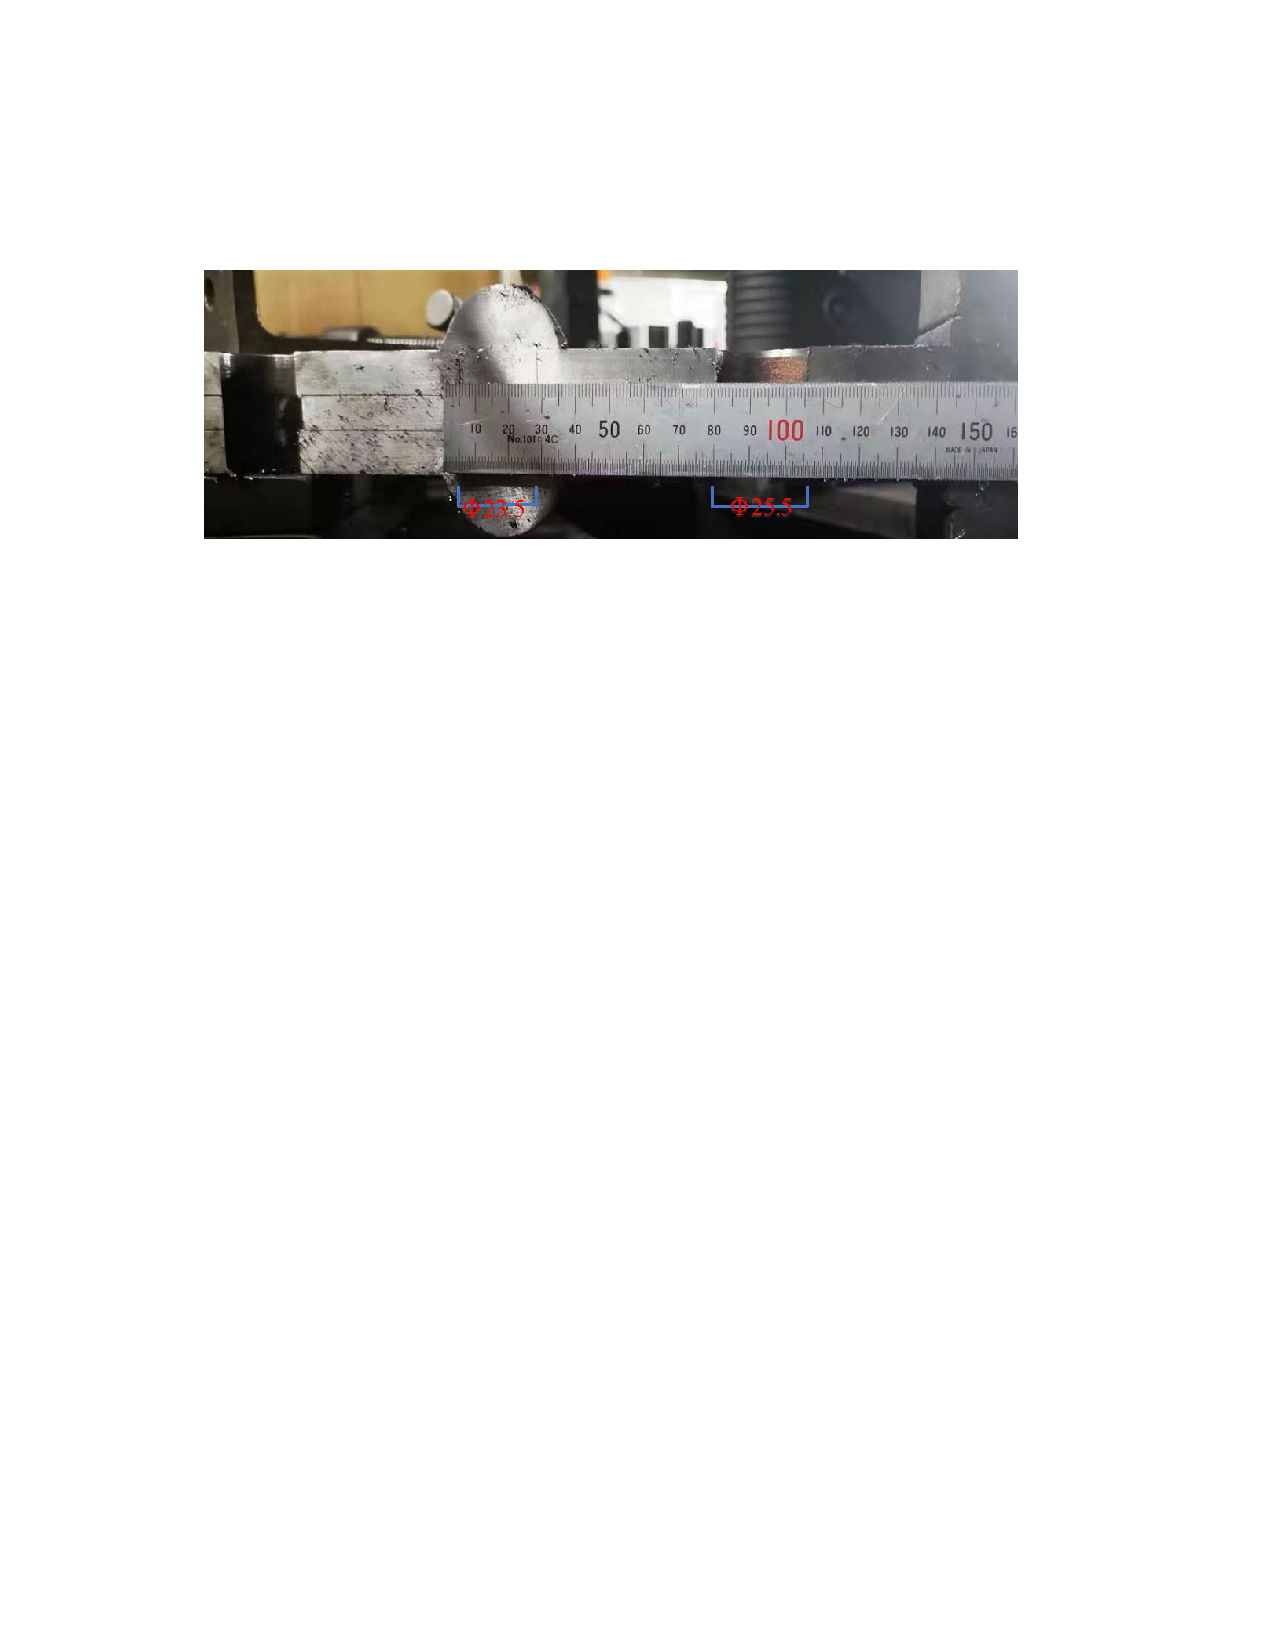
\includegraphics[width=0.8\textwidth]{imgs/ch3/ch3beasta.pdf}
    \caption{Confirm the filling status of the rivets}
    \label{fig-ch3beasta}
\end{figure}


\subsection{Test method}

\subsubsection{Specimens size}

Fig. \ref{fig-sepc-size} shows the specimen shape and detailed dimensions. The 150 mm from one end is where the chuck is clamped.

\begin{figure}[htbp]
    \centering
    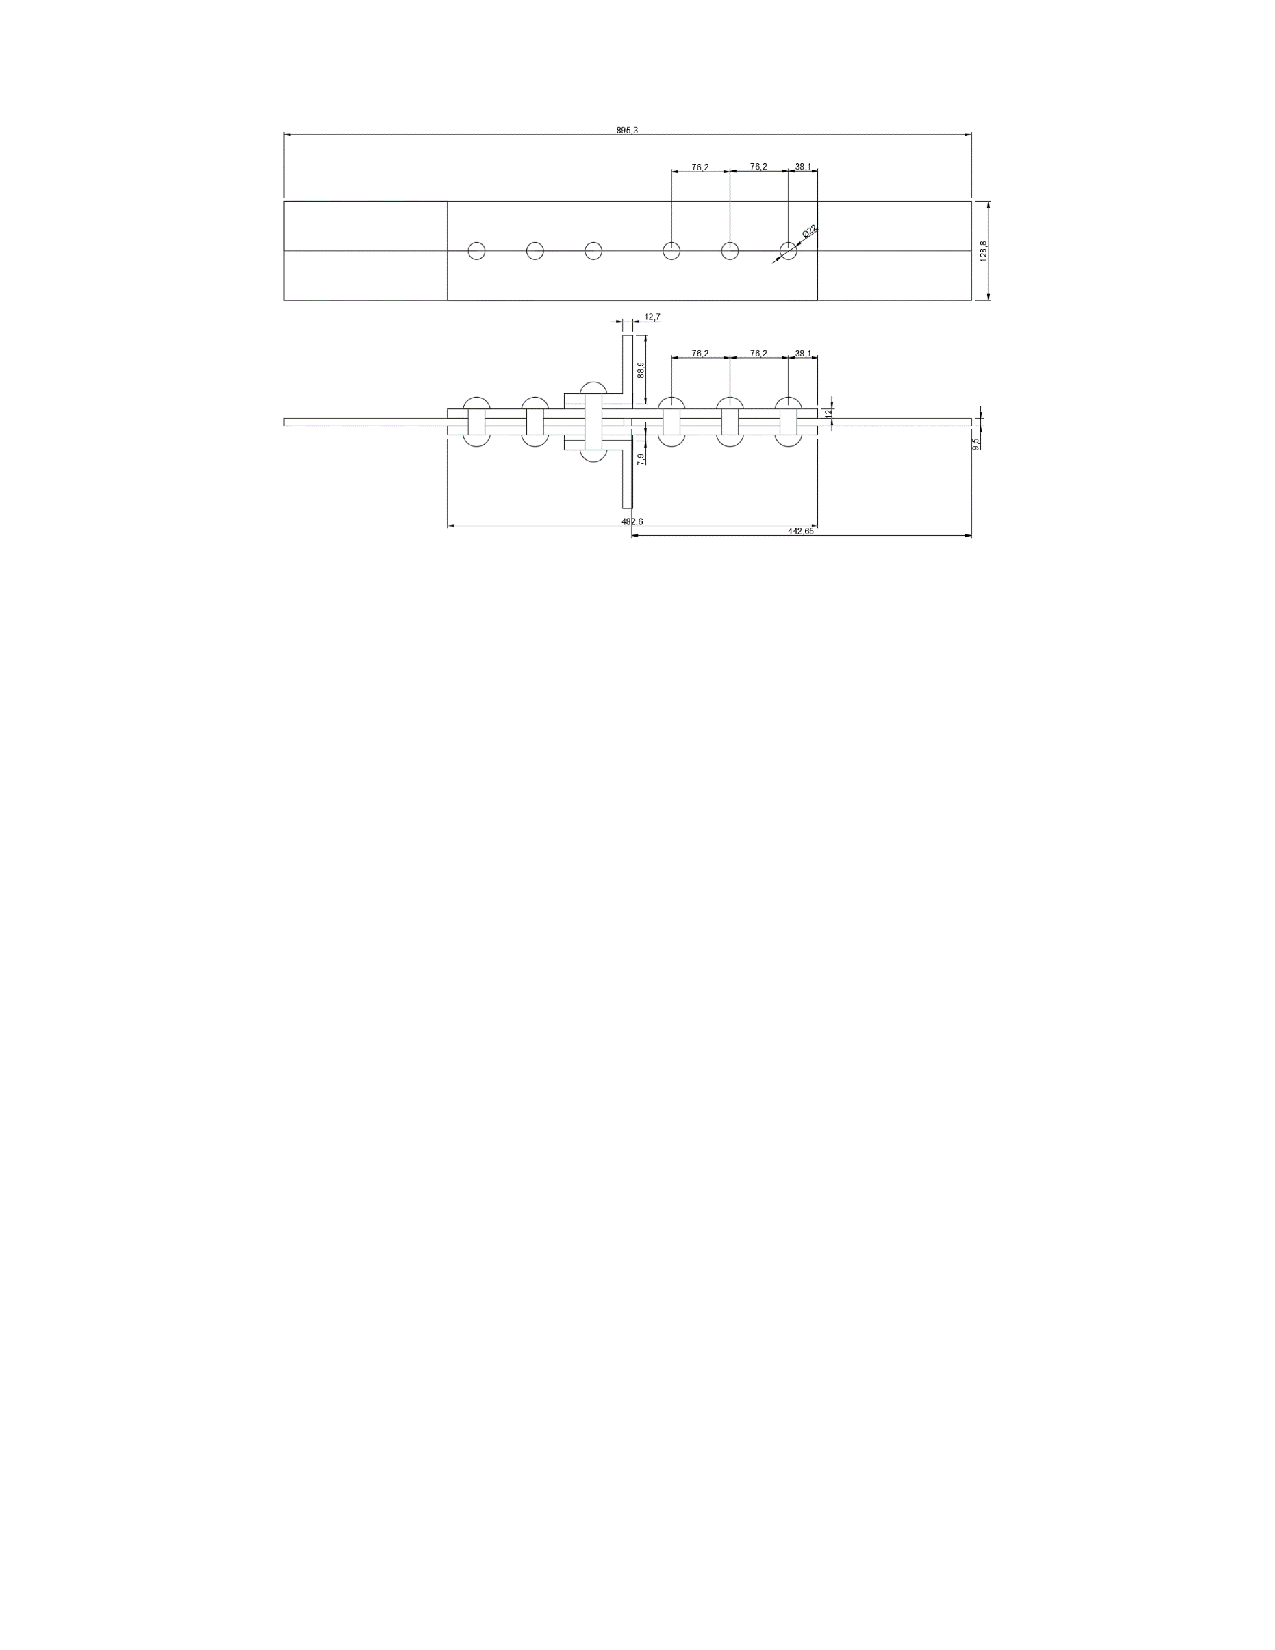
\includegraphics[width=0.8\textwidth]{imgs/ch3/sepc-size.pdf}
    \caption{Specimens size (mm) }
    \label{fig-sepc-size}
\end{figure}

\subsubsection{measurement location}

The measured items were load, preload of bolts, and relative displacement between main plate and splice plate as shwon in Fig. \ref{fig-ch3mealoc}. The bolt preload is measured by strain gauges at the time of assembling all specimens and at the time of the slip test, and the remaining bolt preload at the time of the test is determined to calculate a more accurate slip coefficient, μ. The bolt axial force is measured at the time of assembly, before the slip test, and at the time of slippage. A clip-type displacement transducer is attached to each bolt position to measure the relative displacement of the two splice plates and the main plate. Strain gauges were attached to the outside of the specimen, at the rivet positions, and at the center of the main plate and the splice plate between the hole diameters in order to clarify the load transfer mechanism of the combined joint.

\begin{figure}[htbp]
    \centering
    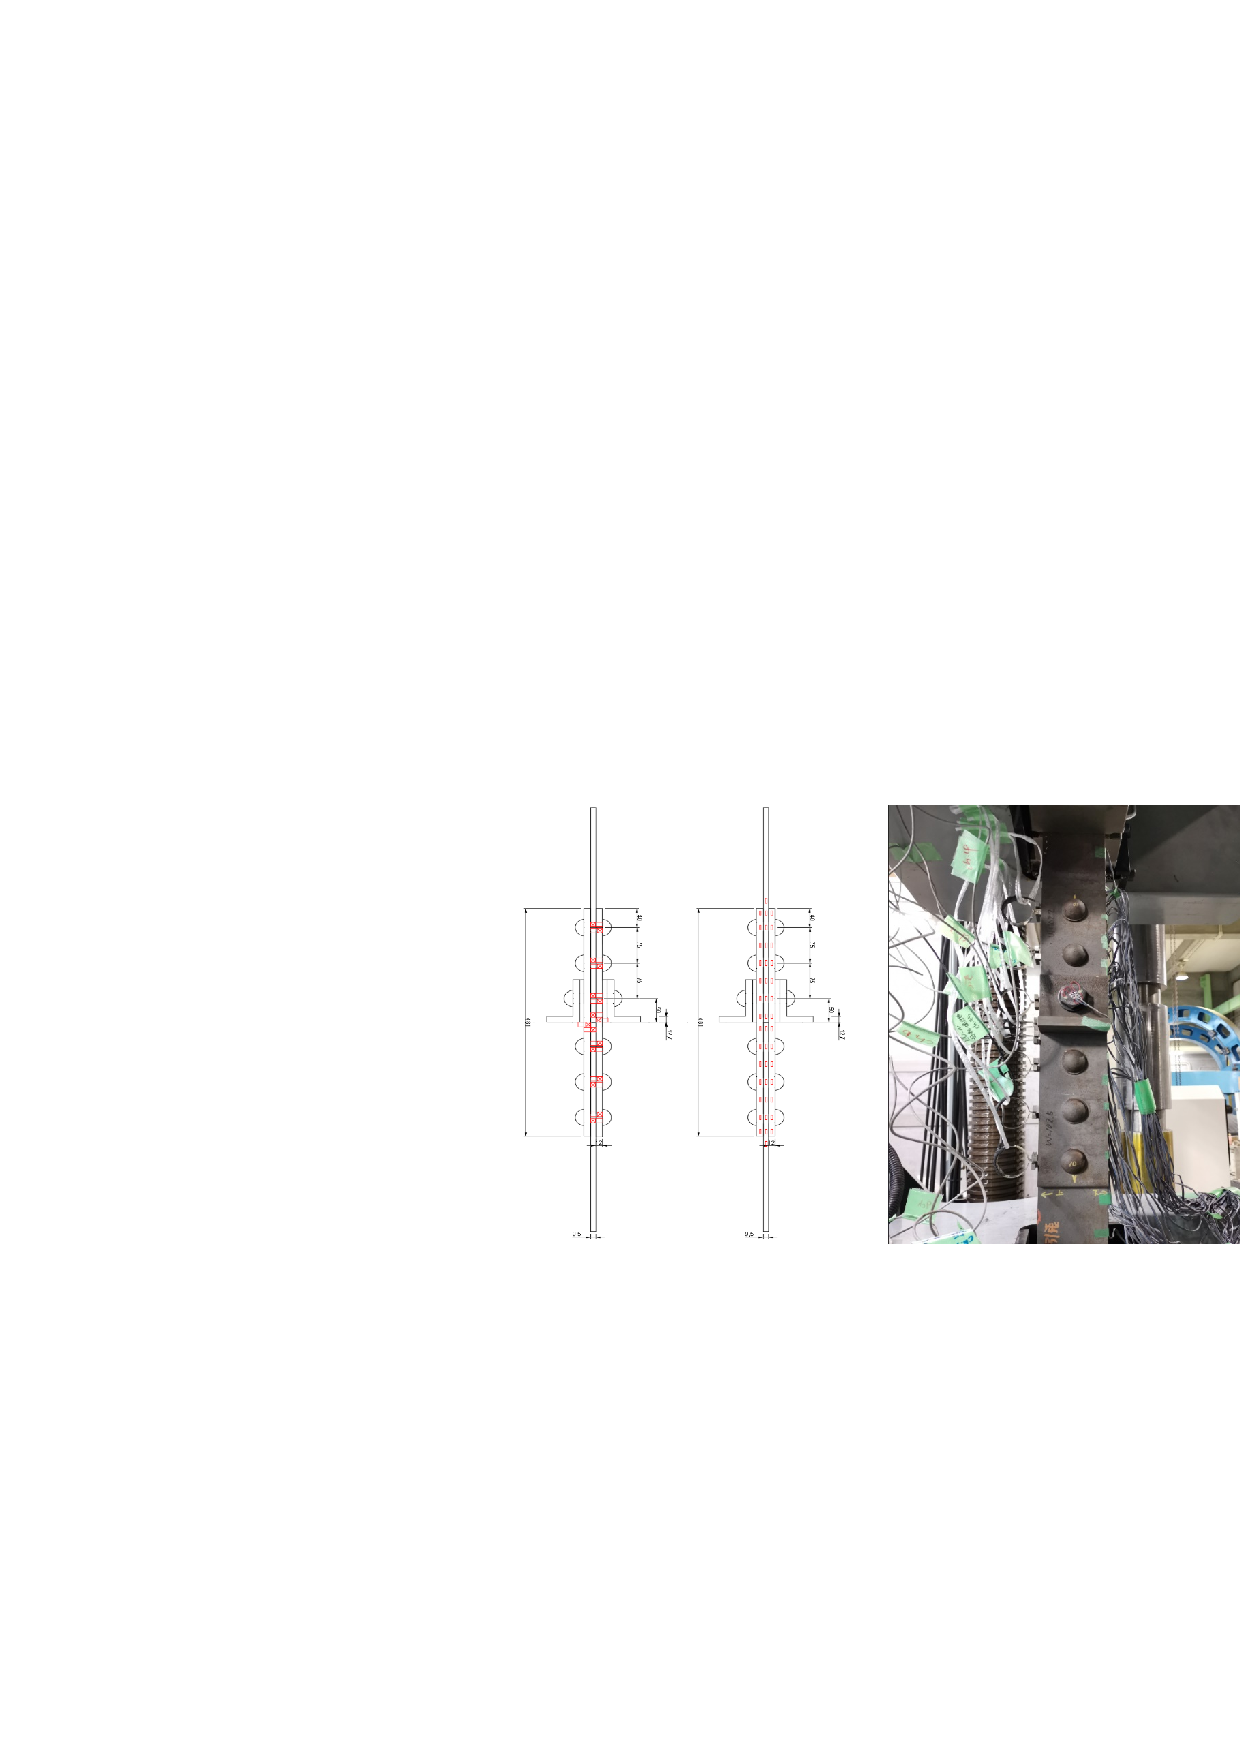
\includegraphics[width=0.8\textwidth]{imgs/ch3/ch3mealoc.pdf}
    \caption{Measurement location}
    \label{fig-ch3mealoc}
\end{figure}

\subsubsection{Test procedure}

When riveted joints were partially or completely replaced with high-strength bolts, F10T (M22) was used as the high-strength bolt for friction joints. The axial force of the tightening bolt was set to 226 kN, which is 1.1 times the design bolt axial force of 205 kN. The period from tightening to the start of the test is one week to allow for the reduction of axial force due to relaxation. A universal testing machine (loading capacity: 2000 kN) owned by Osaka City University was used for the test, and the load was applied until fracture. The loading speed was 1 kN/s, and measurements were taken at 1-second intervals.

\subsubsection{Remove the rivet}

To remove the rivets, the rivet heads on one side were first carefully removed with a disk sander. The joint removed from the actual bridge was already firmly filled with rivets, and the shaft was deformed according to the relative displacement between the plates. Drilling was performed using an Atra-Ace. Enlarged holes were drilled using a jet broach with a diameter of 26.5 mm, aligned with the center of the rivet shaft. The rivet shaft was pressed out while the four corners of the plate were fixed to prevent the plate from disassembling due to rivet removal. The tools used are shown in Fig.\ref{fig-retool}.

\begin{figure}[htbp]
    \centering
    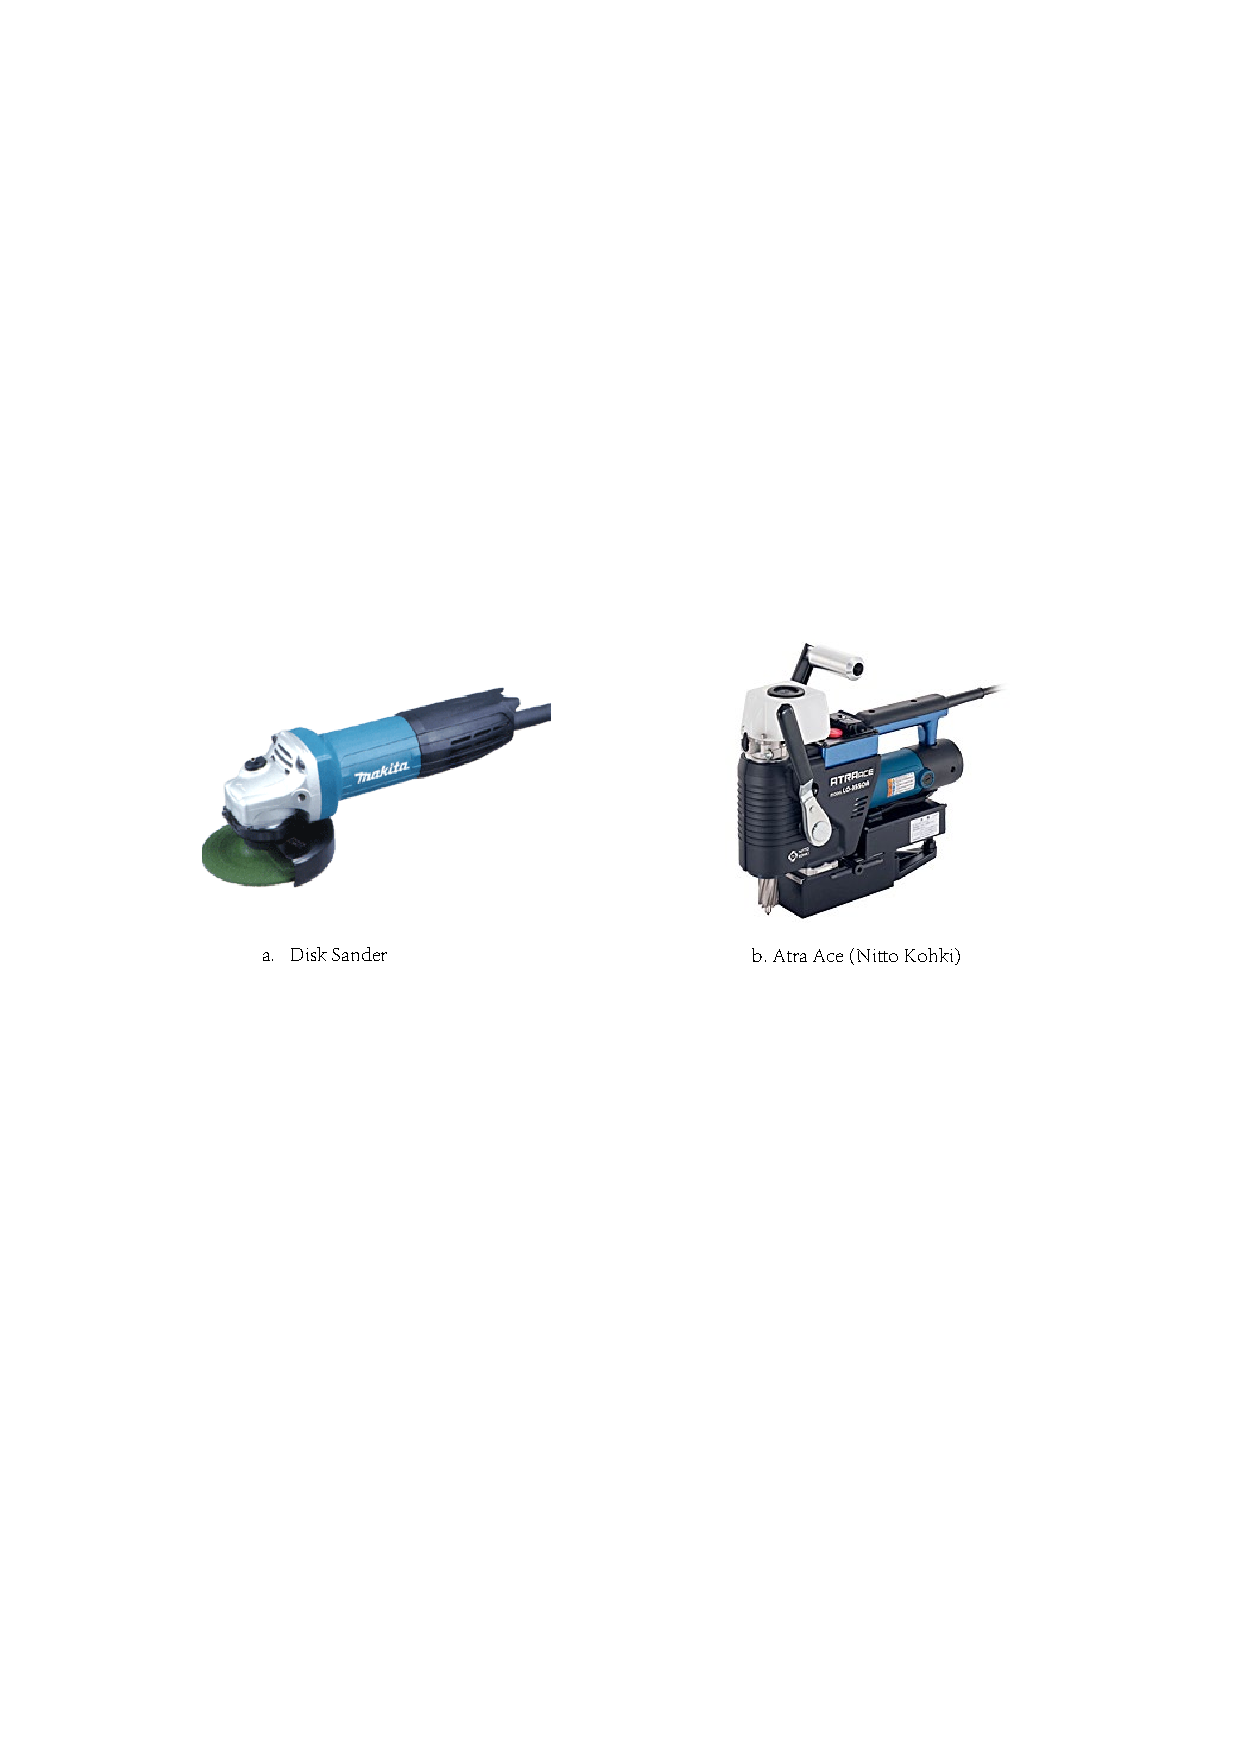
\includegraphics[width=0.8\textwidth]{imgs/ch3/retool.pdf}
    \caption{Tools for rivet removal}
    \label{fig-retool}
\end{figure}

When replacing rivets, loads may be concentrated on specific rivets or high-strength bolts during the replacing process, which can be dangerous. In the present replacement work, the order in which the sharing ratio is relatively equal (\#1 → \#6 → \#2 → \#5 → \#3 → \#4) (the bottle order was set from the edge end of one side of the joint to the edge end of the other side of the joint) according to the study by Kakimoto et al. \cite{kakimoto2002Mechanical} was followed.  The replacement process is shown in Fig. \ref{fig-reproce}.

\begin{figure}[htbp]
    \centering
    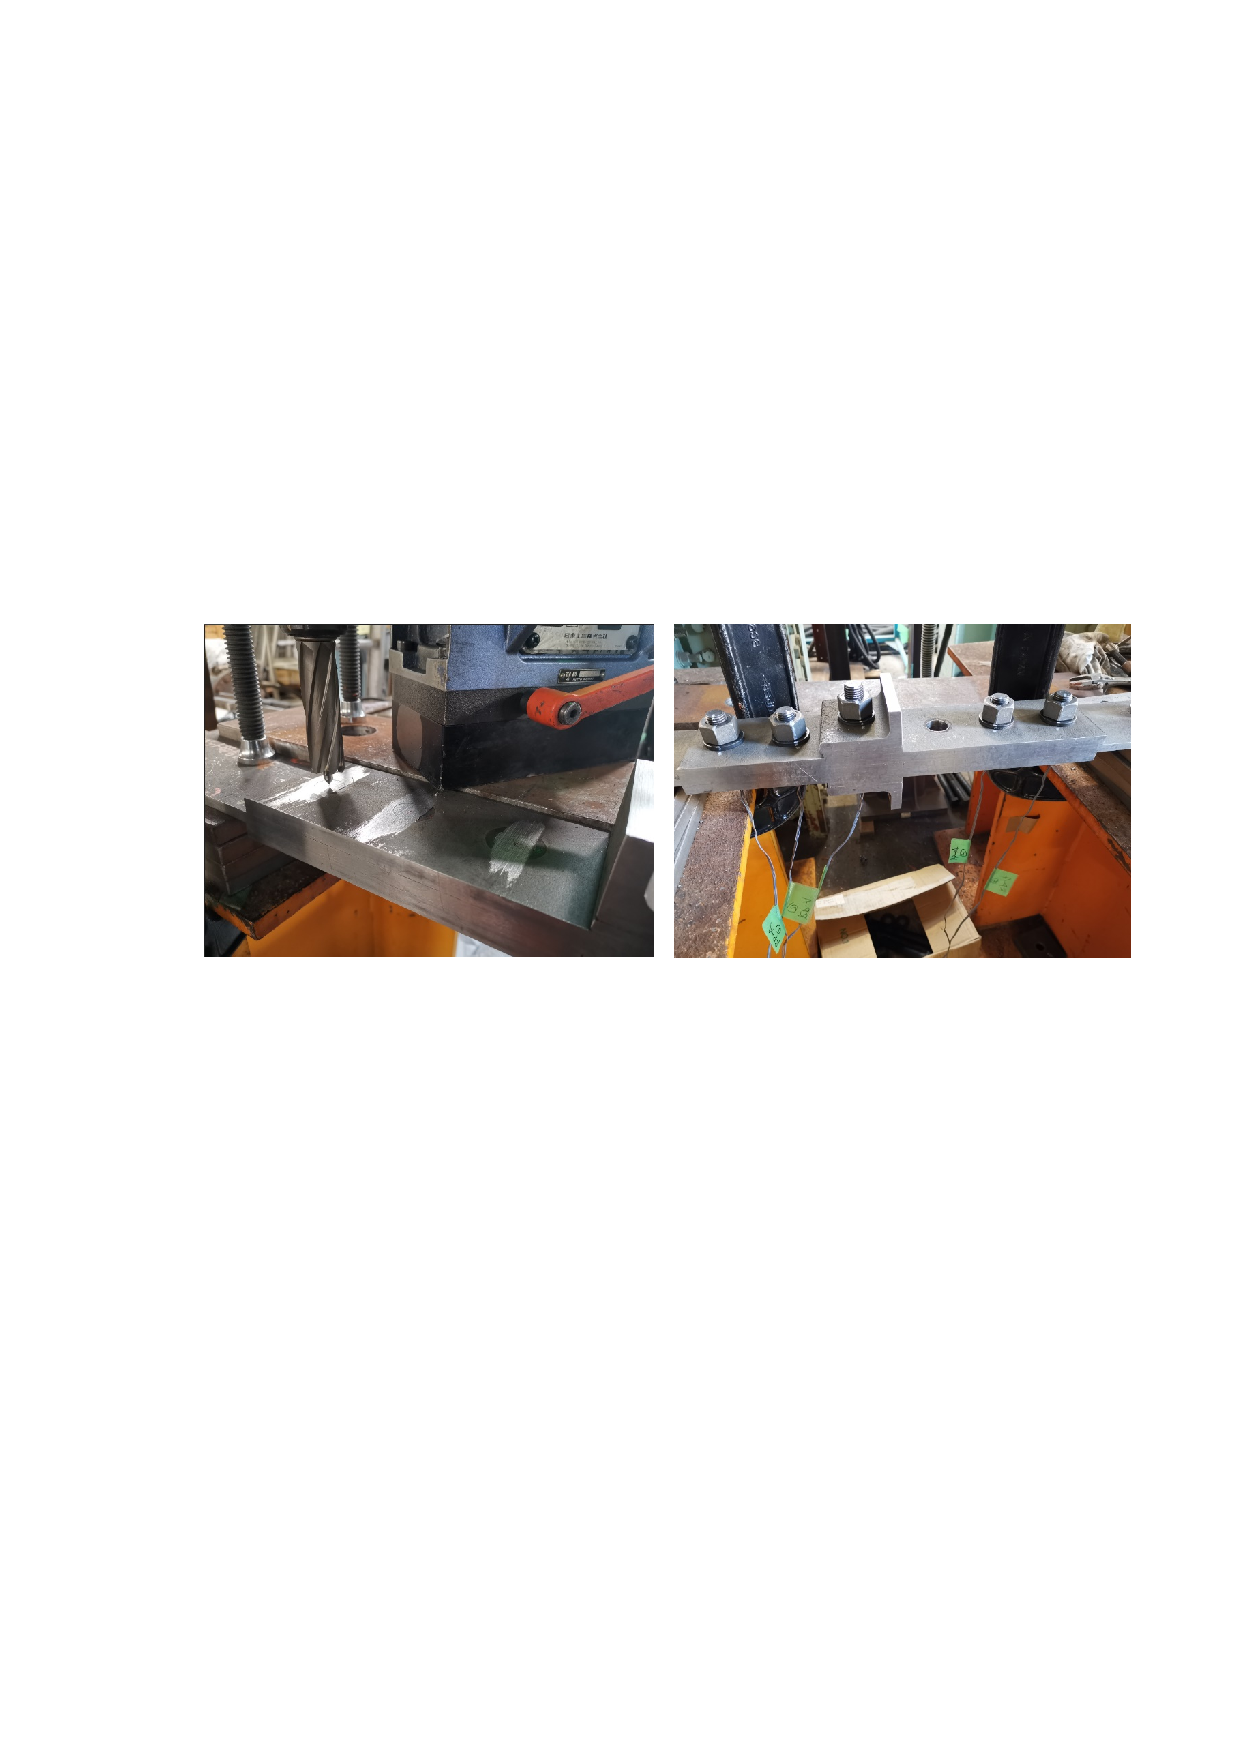
\includegraphics[width=0.8\textwidth]{imgs/ch3/reproce.pdf}
    \caption{Replacement process}
    \label{fig-reproce}
\end{figure}

\subsubsection{Designed resistance of the joint}

small-scale slip tests on the cross girder of the Dojima Bridge yielded an average slip coefficient of 0.21, which is smaller than in previous studies. This value is smaller than previous studies. Here, the design resistance was evaluated using the slip coefficient of 0.21, which is the result of the small-slip test.

The design thickness of the main plate of the subject joint was 9.5 mm, and the thickness of the base material varied widely due to the limited manufacturing technology of steel products at that time. The average thicknesses of the main plates taken from the same girder are 9.3 and 10.2, respectively.
The average thicknesses of the main plates taken from the same girder are 9.3 and 10.2, respectively. The design bearing capacity was calculated using the thickness of each joint.

The slip coefficient is calculated by the following equation.

\begin{equation} \label{eq-fs}
    F_{sd} = n m \mu_d N
\end{equation}

where, n is the number of bolts, m is the number of the friction plane, $\mu_d$ is the slip coefficient, and $N$ is the design bolt perload.

The net sectional yield resistance $F_{yd}$ and net sectional ultimate resistance $F_{ud}$ of the main plate are calculated by Eq.\ref{eq-fyd} and \ref{eq-fud}, respectively, without taking into account the effect of bolt axial force.

\begin{equation}\label{eq-fyd}
    F_{yd} = (w - d) t f_y
\end{equation}

\begin{equation}\label{eq-fud}
    F_{ud} = (w - d) t f_u
\end{equation}

Where, $w$ is the width of the main plate, $d$ is the hole diameter, $t$ is the thickness of the main plate, $f_y$ is the yield resistance of the main plate, and $f_u$ is the ultimate resistance of the main plate.

The design value of the slip/yield resistance ratio, βd, was calculated using Eq. \ref{eq-beta}.

\begin{equation}\label{eq-beta}
    \beta_d = \frac{F_{sd}}{F_{yd}}
\end{equation}

Bearing resistance is calculated with reference to the equation of RTRI, Japan \cite{rtri1992Manual}.

\begin{equation}
    F_{b,RTRI} = 1.5 d t f_y
\end{equation}

The strength of hybrid joints is obtained by accumulating slip strength and bearing resistance.

\begin{equation}
    F_{hybrid} = F_{sd} + F_{b,RTRI}
\end{equation}

The rivets are red-hot rivets that are tightened with a hammer to form a dome-shaped rivet head. It is known that cooling the rivet introduces axial force, and the axial force of the rivet was taken into account when calculating the slip capacity. The axial force of a rivet with a diameter of 22 mm and a shaft length of 34 mm has an average axial force/yield strength ratio of 0.4, based on previous studies. 75 mm shaft length is said to be 70\% of the rivet shaft yield value. Since the average yield strength of the rivets used in the Dojima Bridge is 295 Mpa , we considered that the rivets with a shaft length of 34 mm and a shaft length of 75 mm introduced an axial force of about 45 kN and 78.5 kN, respectively.

The design resistance of the joint are summarized as in Table \ref{tab-designres-ch3}.

\begin{table}[]
    \centering
    \caption{Design resistance of the joint}
    \label{tab-designres-ch3}
    \begin{tabular}{@{}cccccccc@{}}
        \toprule
        \multirow{2}{*}{} &
          \multicolumn{2}{c}{\begin{tabular}[c]{@{}c@{}}Preload of rivet\\ kN\end{tabular}} &
          \multirow{2}{*}{\begin{tabular}[c]{@{}c@{}}Applied \\ preload\\ kN\end{tabular}} &
          \multirow{2}{*}{\begin{tabular}[c]{@{}c@{}}Slip\\ resistance\\ $F_s$\end{tabular}} &
          \multirow{2}{*}{\begin{tabular}[c]{@{}c@{}}Net C-S yield\\ resistance\\ $F_{yd}$ kN\end{tabular}} &
          \multirow{2}{*}{β} &
          \multirow{2}{*}{\begin{tabular}[c]{@{}c@{}}Net C-S Ultimate\\ resistance\\ $F_{ud}$\end{tabular}} \\ \cmidrule(lr){2-3}
              & 33mm                & 75mm                  &       &        &        &      &       \\ \midrule
        RIVET & \multirow{4}{*}{45} & \multirow{4}{*}{78.5} & -     & 70.77  & 197.23 & 0.36 & 324.3 \\
        RP1   &                     &                       & 214.9 & 142.13 & 193.28 & 0.74 & 318.8 \\
        RP2   &                     &                       & 215.5 & 142.37 & 199.12 & 0.72 & 331.4 \\
        RP3   &                     &                       & 217.5 & 201.63 & 194.08 & 1.04 & 320.8 \\
        RPALl & \multicolumn{2}{c}{-}                       & 215.5 & 271.53 & 190.59 & 1.42 & 315.3 \\ \bottomrule
    \end{tabular}
\end{table}

\subsection{Test results and discussion}

\subsubsection{Overall test results}

Fig.\ref{fig-3-10} shows the relationship between load and displacement for the five specimens. Since the net sectional yield capacity of each case is different, the loads are non-dimensionalized by the respective net sectional yield capacity, Py. The displacements are the displacements between the fixtures.

Fig.\ref{fig-3-10} shows that RP1 (replacing the outer rivets with high-strength bolts), RPall (replacing all rivets), and the repaired case with two rivets replaced had almost the same yield strength. In the case where two rivets were replaced, the slope of the load-total displacement relationship changed at about 1.1 times the yield capacity, confirming the effect of the yielding of the pure section of the main plate.

\begin{figure}[htbp]
    \centering
    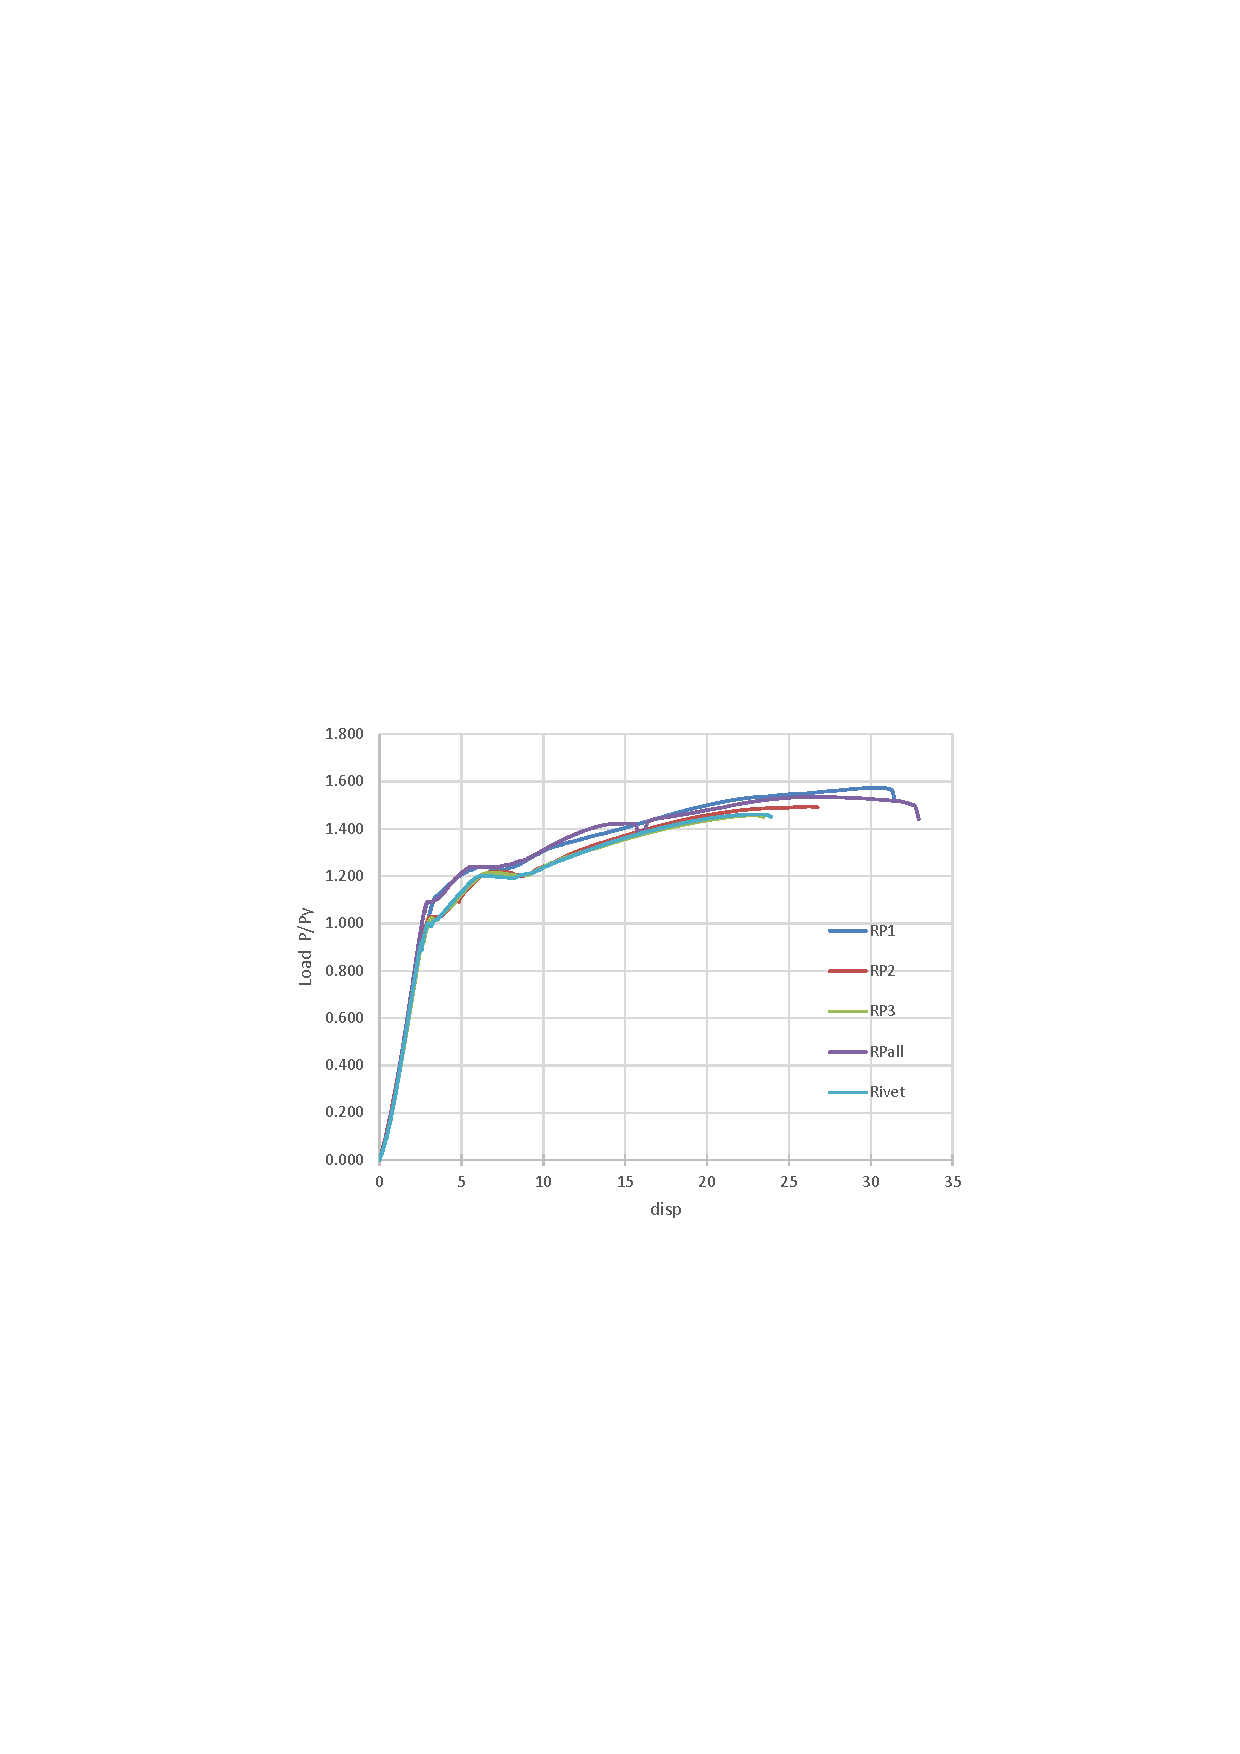
\includegraphics[width=0.7\textwidth]{imgs/ch3/fig3-10.pdf}
    \caption{The relationship between load and displacement for the five specimens}
    \label{fig-3-10}
\end{figure}

The RP1 and RPall cases tend to have a smaller overall displacement with respect to the load than the other cases. As shown in Fig.\ref{fig3-11}, yielding occurred at 1.09 for the RP1 and RPALL cases, and the net section yielding capacity occurred at 1.02 and 1.015 for the RP2 and RP3 cases, respectively. The Rivet case in sound condition was found to yield at position 1, as in the steel tensile test. This is considered to be because the axial force of the rivet is smaller than in the other cases, resulting in less load transfer to the splice plate.


Fig.\ref{fig3-12} shows the relationship between load and relative displacement at the net cross-sectional position. 1.09, the same value as the load-strain relationship, was observed for RPALL.

\begin{figure}[htbp]
    \centering
    \begin{minipage}[t]{0.42\textwidth}
    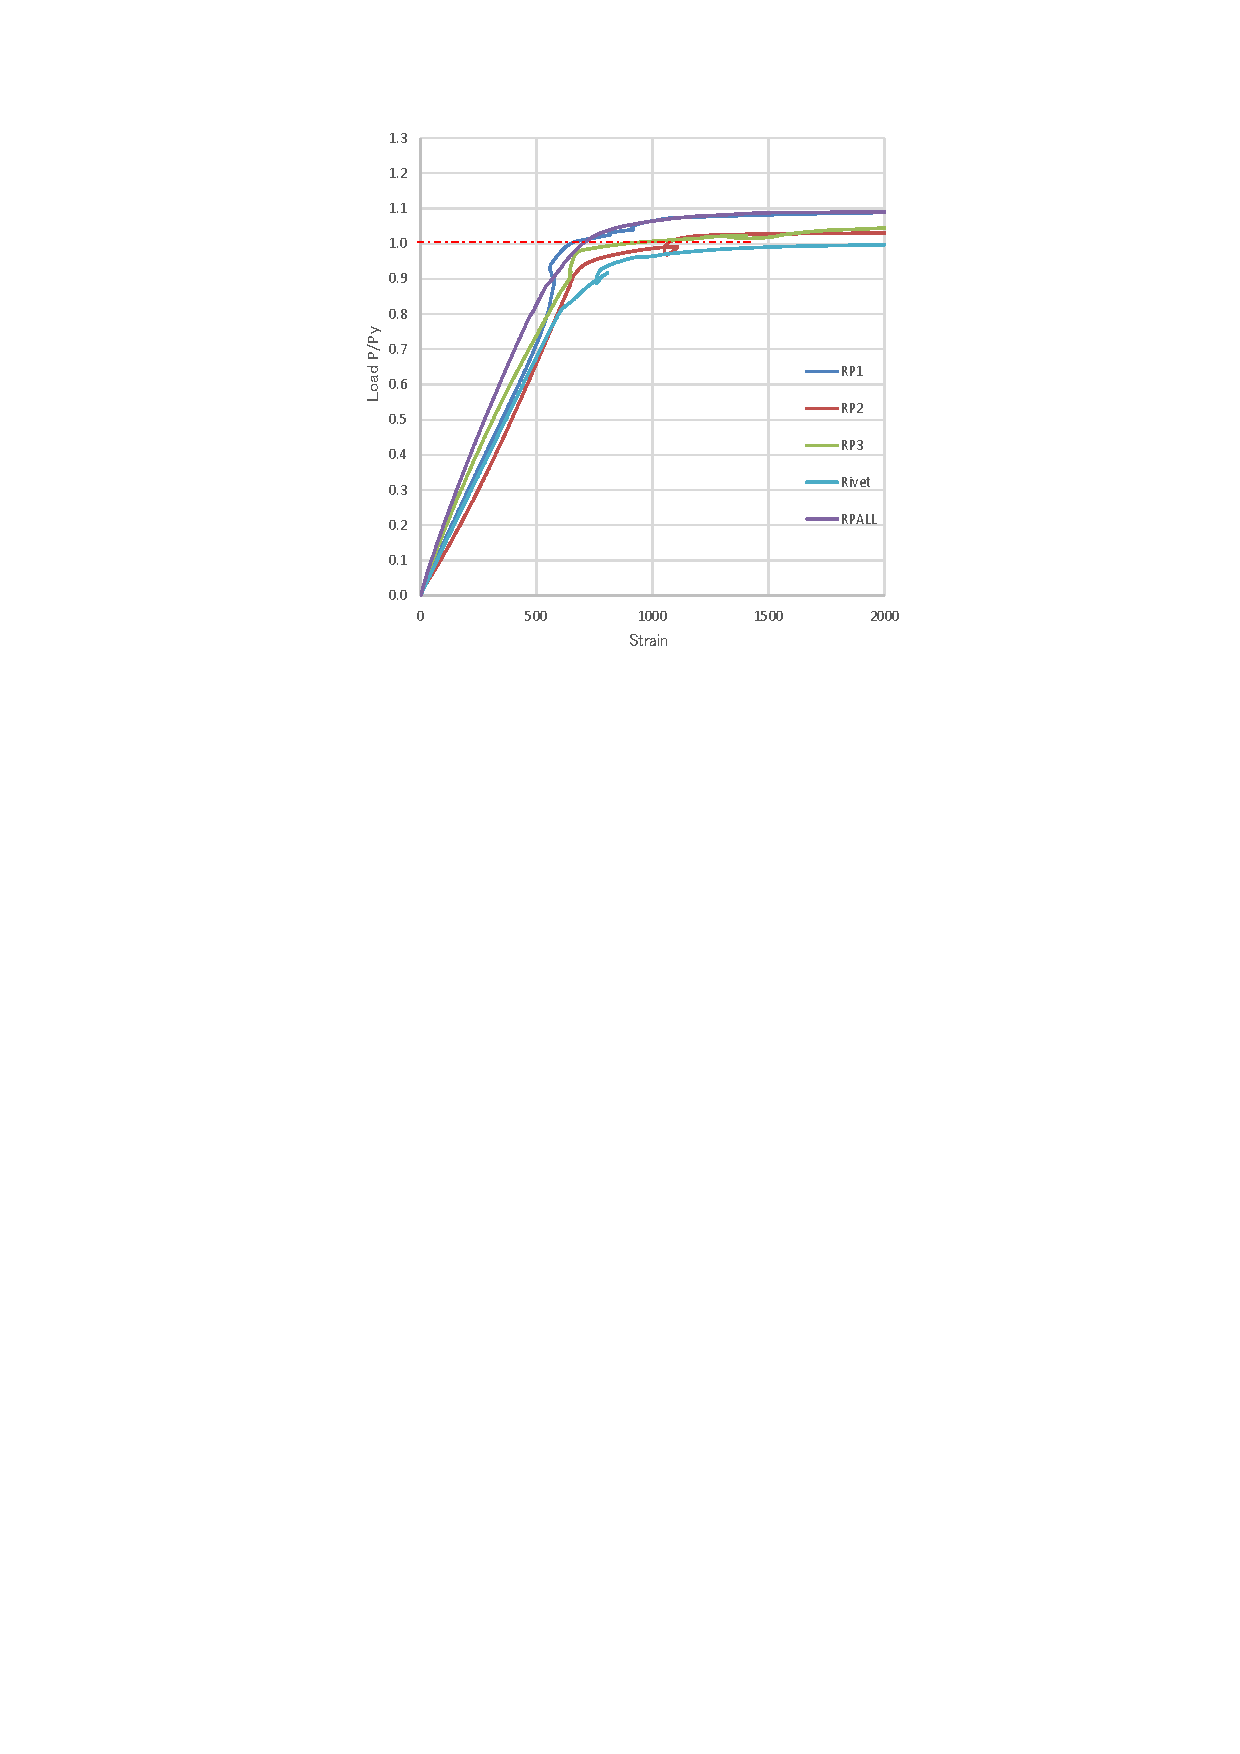
\includegraphics[width=\linewidth]{imgs/ch3/fig3-11.pdf}
    \caption{The relationship between Load and Strain, Net cross-section position (Hole \#1)}
    \label{fig3-11}  
    \end{minipage}
    \begin{minipage}[t]{0.42\textwidth}
    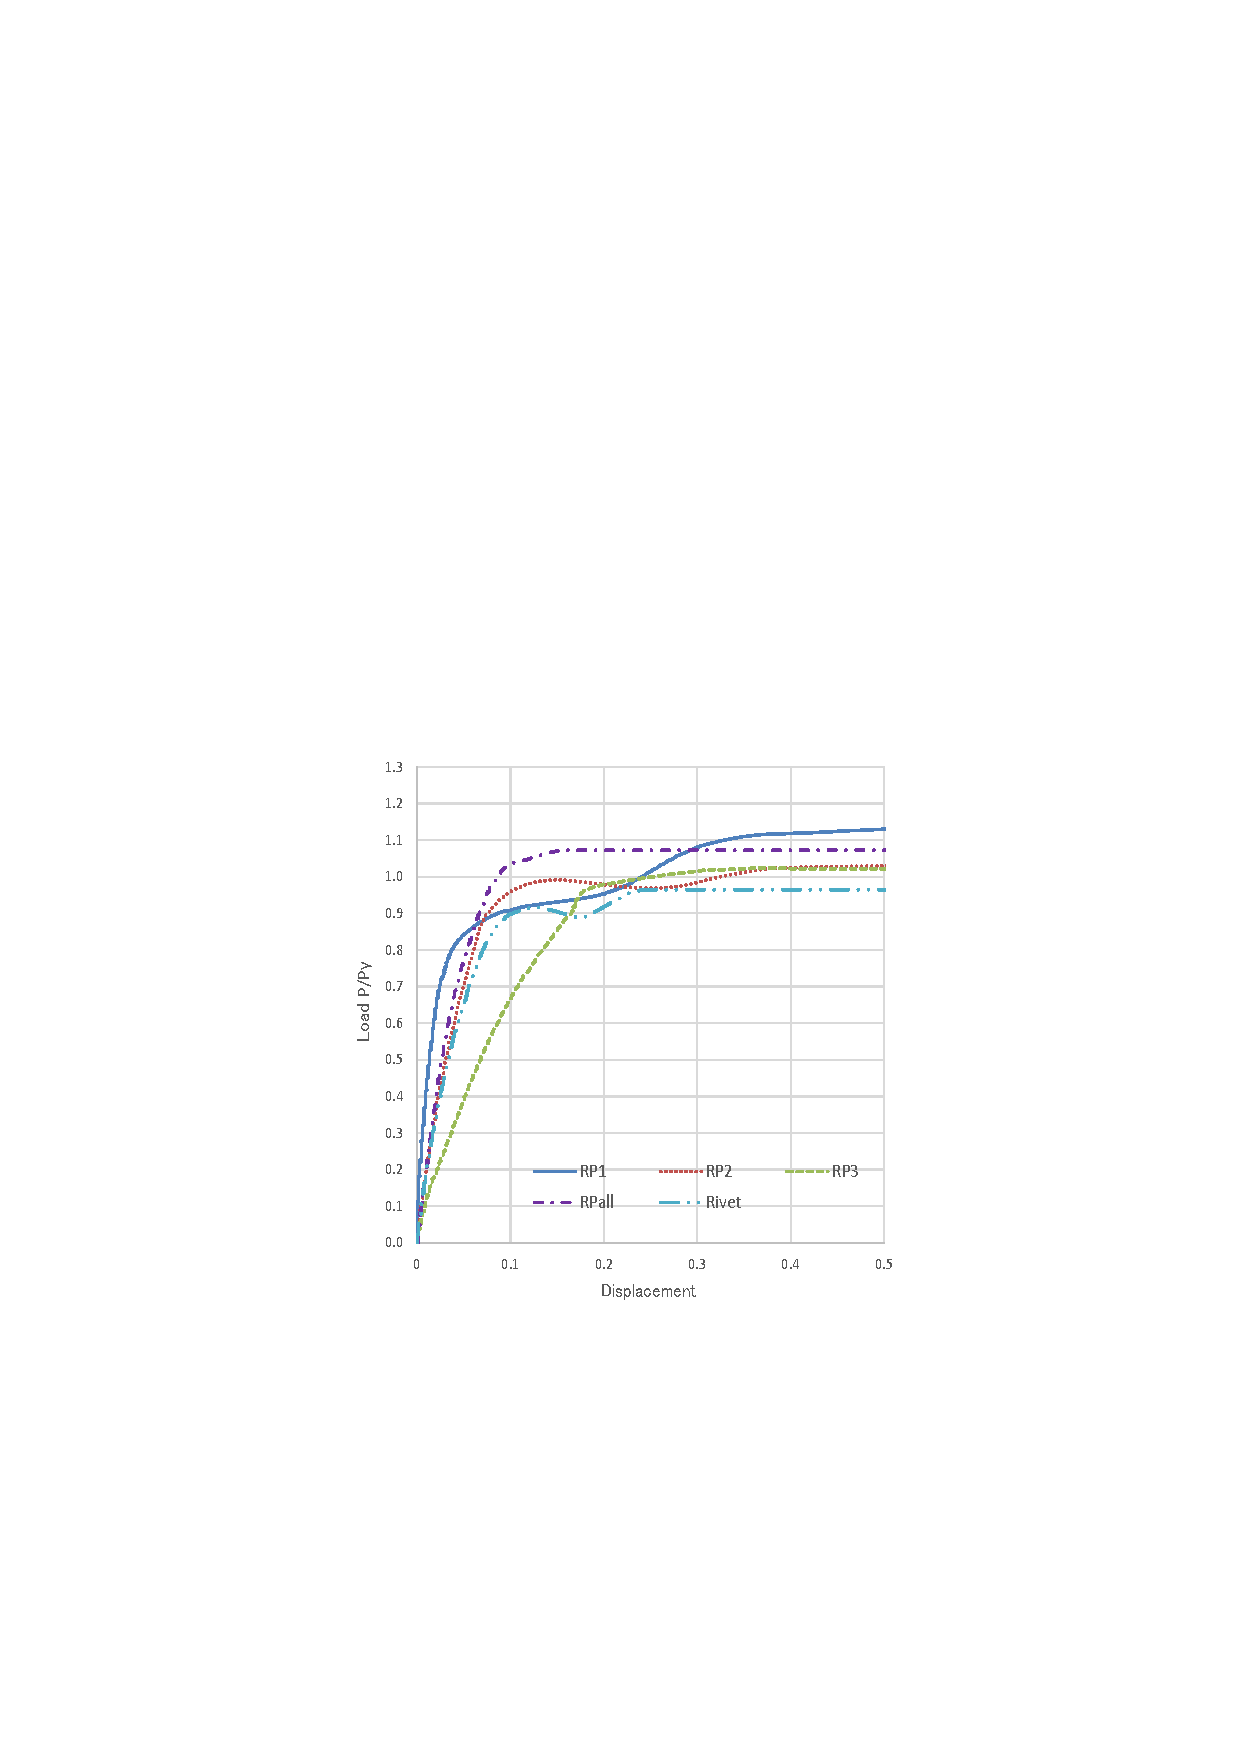
\includegraphics[width=\linewidth]{imgs/ch3/fig3-12.pdf}
    \caption{The relationship between Load and Displacement, Net cross-section position (Hole \#1)}
    \label{fig3-12}  
    \end{minipage}
\end{figure}

It was confirmed that the frictional force caused by the introduction of the high-strength bolt axial force transfers the load from the main plate to the splice plate. Fig.\ref{fig3-13} shows the load sharing ratio between the splice plate and the main plate. As shown in Fig.\ref{fig3-13}, when the load reached the net sectional yield, the load transfer ratio to the splice plate was 15\% for the RP1 case, and the transfer ratio was 5\% for the RPALL full replacement case, raising the net sectional yield capacity by 13\% and 8\%, respectively. This is due to the difference in the slip coefficient and the difference in the slip capacity of a single bolt.

The frictional force of a single RP1 outer bolt is 146.13 kN, which is about 1.6 times higher than the RPALL frictional force of 89.16 kN. the rate of increase of the RP1 quasi-sectional yield capacity is also higher than that of the RPALL by a factor of 1.6. It was found that the frictional force of the single bolt on the outside of the joint is directly proportional to the yield capacity of the pure section. In addition, the friction force between the quasi-sections of The increase in quasi-sectional yield capacity for RP2 and RP3 was 1.02 and 1.015, respectively, which was attributed to the fact that the adjacent high-strength bolt transmitted a higher clamping force than the rivet. The axial force of the adjacent high-strength bolts should be considered in terms of the specific influence range and axial force relationship.


\begin{figure}[htbp]
    \centering
    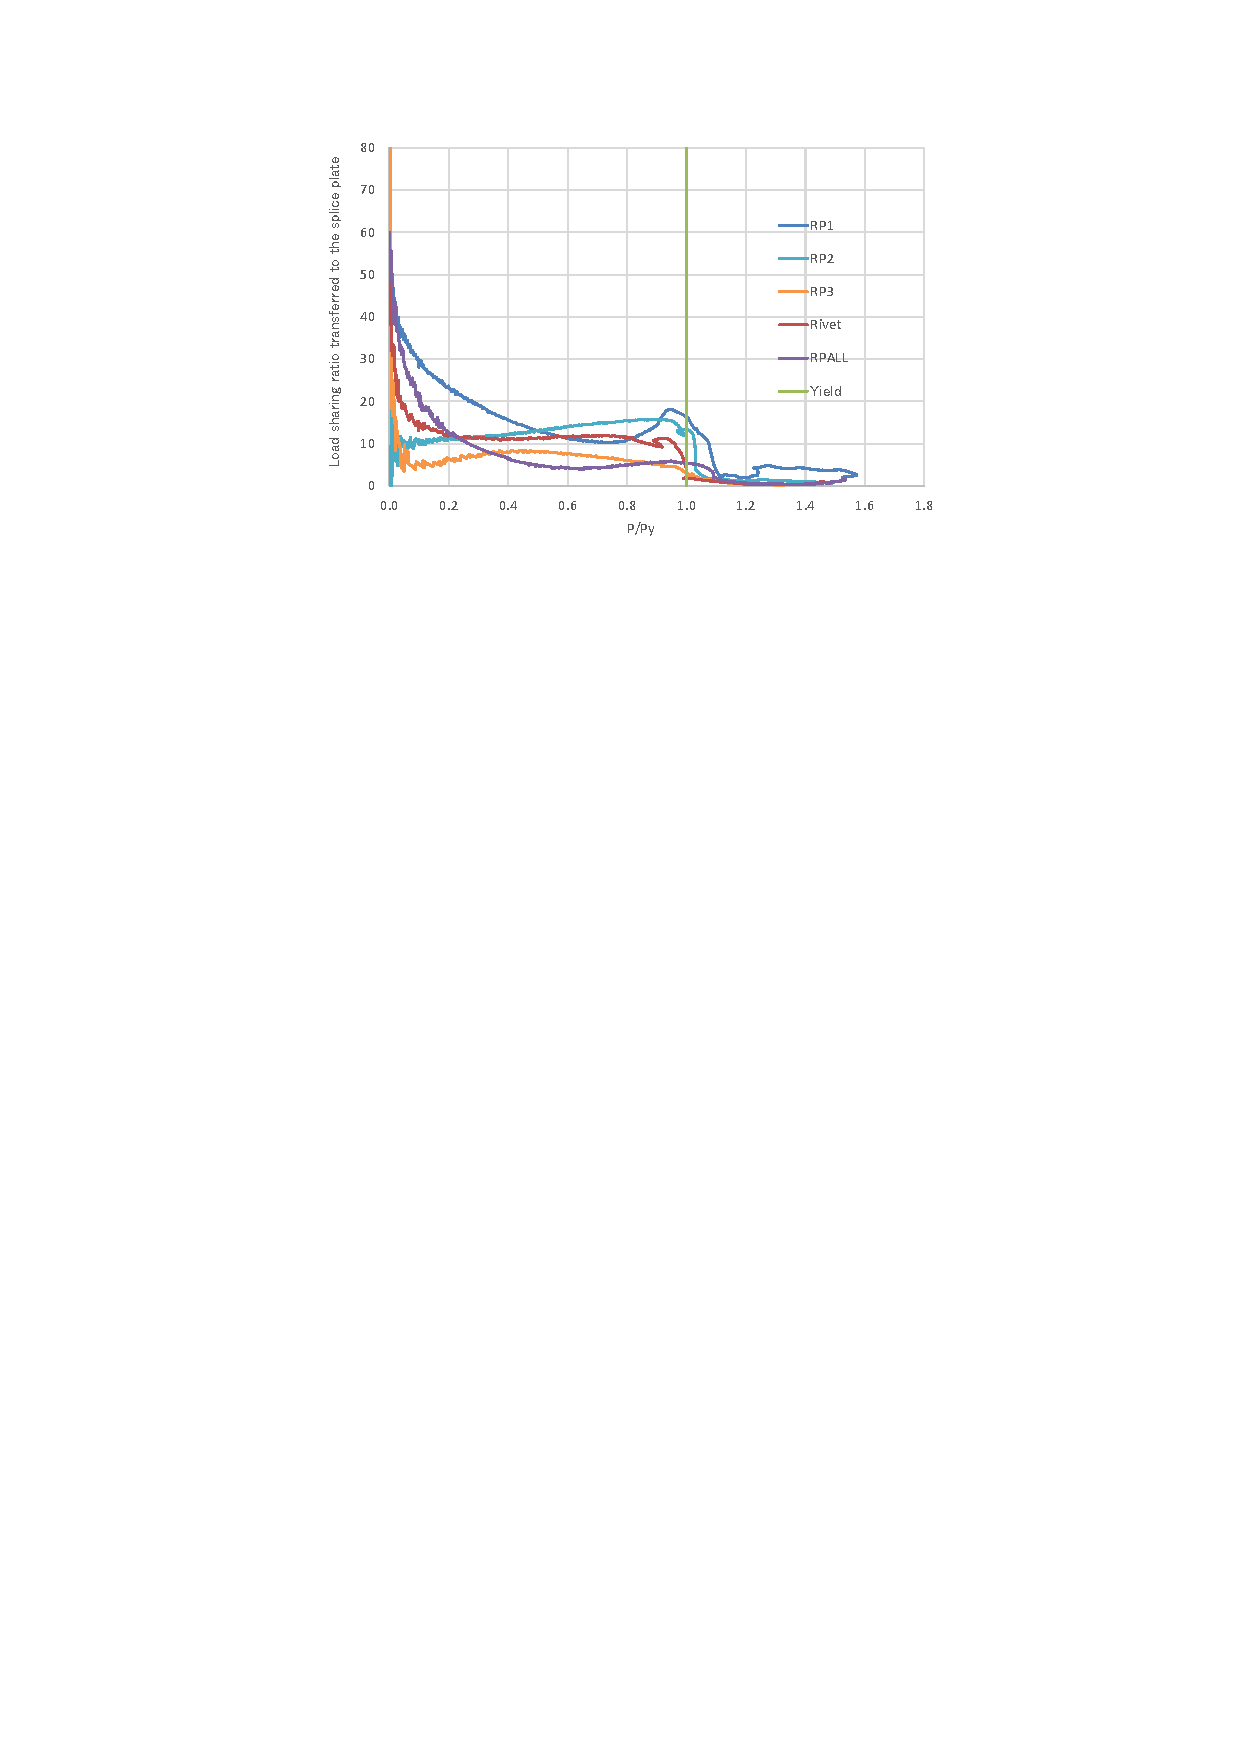
\includegraphics[width=0.7\textwidth]{imgs/ch3/fig3-13.pdf}
    \caption{the load sharing ratio between the splice plate and the main plate}
    \label{fig3-13}
\end{figure}

Fig.\ref{fig3-15} shows the load-relative displacement relationship measured at 10mm away from the gap, RPALL is almost equal to the calculated sliding load of 271 kN. This is because the slip load is determined by the relative displacement between the base metal and the attached plate at 10 mm from the gap, which is affected by the tightening of the inside bolt. The frictional force of the outer bolt of RP1 is not very useful for the inner rivet because the inner rivet is resisted by the bearing pressure of the inner rivet, and the slip load is larger in the case where the inner bolt of RP3 is replaced. This is considered to be due to the joint resistance of the frictional force of the high-strength bolt and the rivet.

\begin{figure}[htbp]
    \centering
    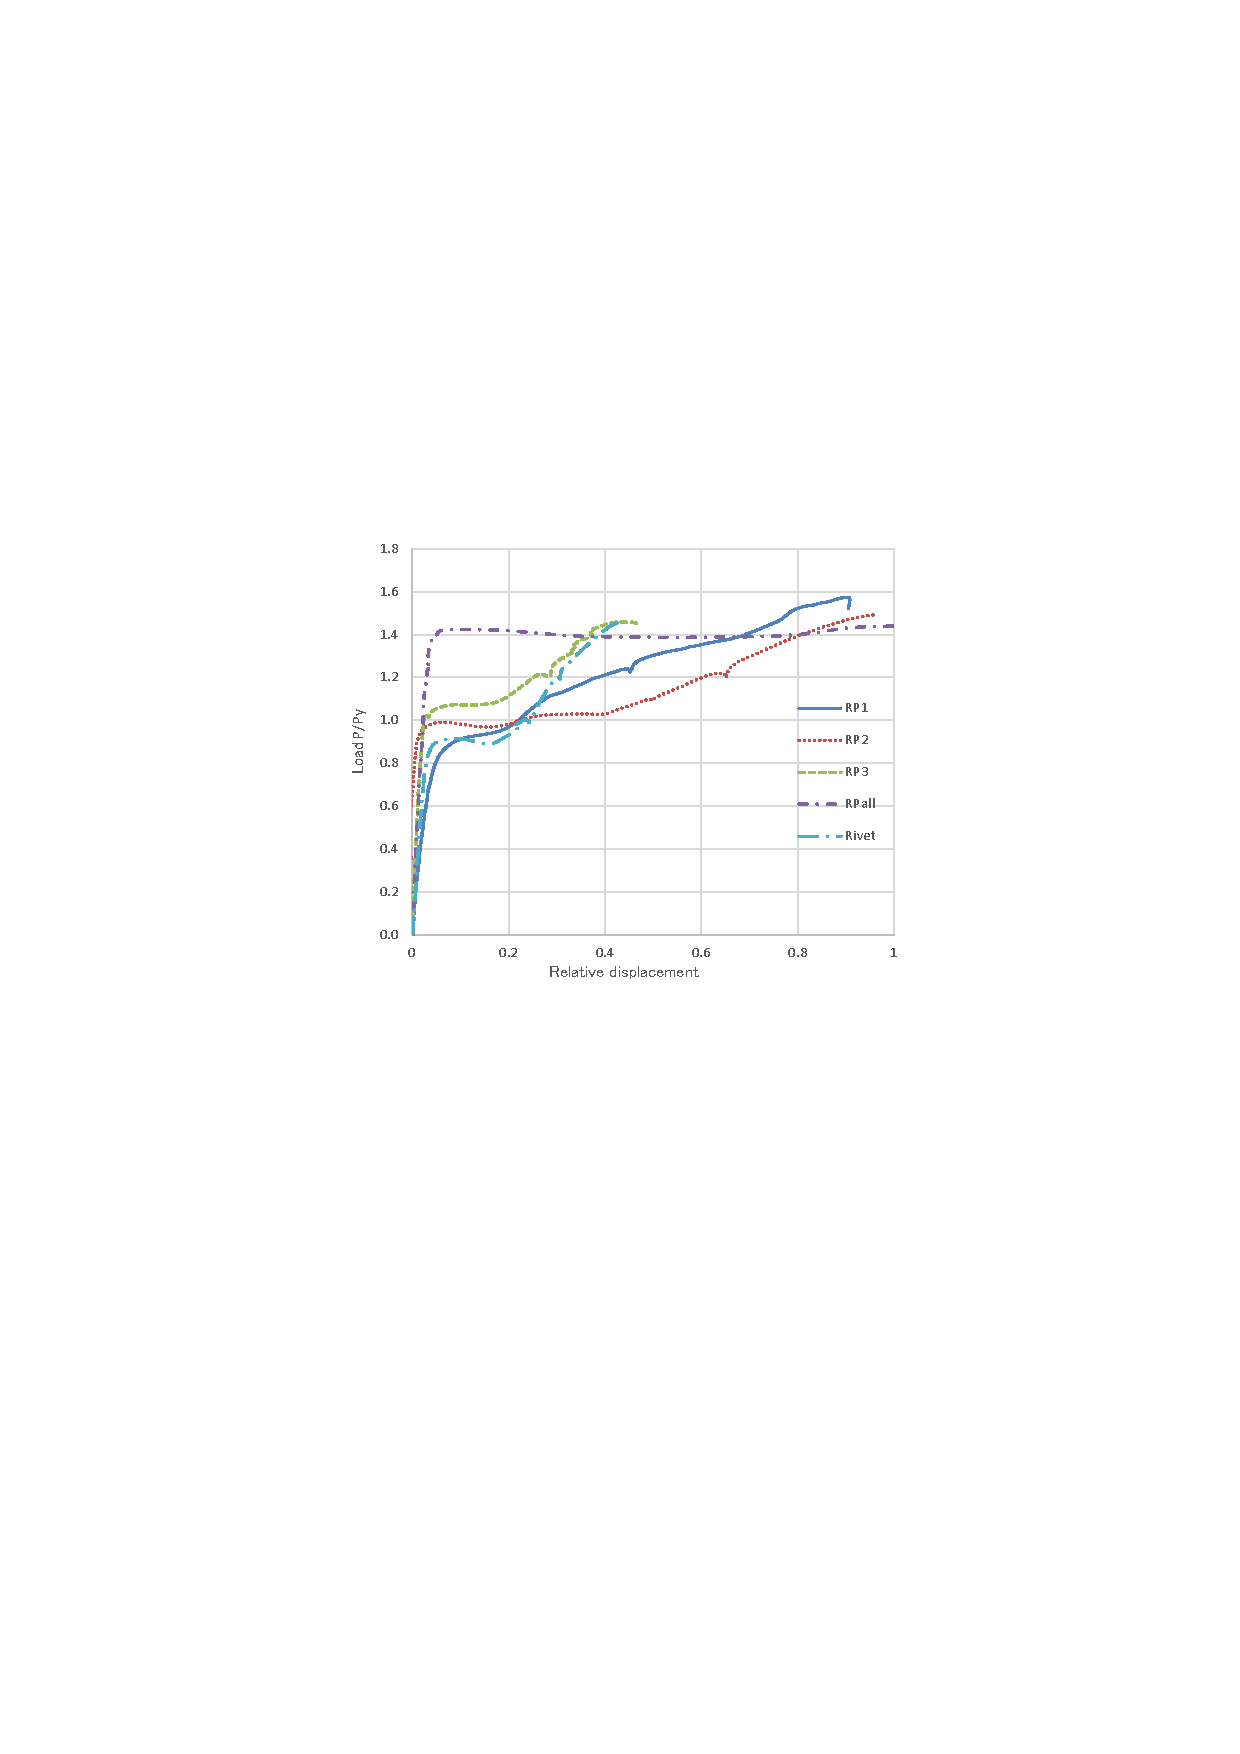
\includegraphics[width=0.7\textwidth]{imgs/ch3/fig3-15.pdf}
    \caption{the load-relative displacement relationship measured at 10mm away from the gap}
    \label{fig3-15}
\end{figure}


Comparison of the experimental and design values of the joint capacity is shown in Table \ref{tab-ch3compare}. The riveted quasi-sectional yield load in the sound condition is almost consistent with the design value. The yielding of the bolt hole in the base metal increased by 1.3\%, 7.9\%, and 0.5\%, respectively, compared to the riveted sound condition, depending on the position of the replacement bolt. It is considered that the replacement of the rivet can relieve the bearing pressure of the rivet by transferring the load to the splice plate, which is fixed by the frictional force of the high-strength bolt, and further to the splice plate by the crimping force, instead of sharing the bearing pressure next to the rivet. In either case, the bearing capacity of the rivet is not reduced. However, when a rivet is removed under dead or live load, the load may concentrate on other rivets, creating a dangerous situation. The reason why the maximum load of the rivet in sound condition is only 0.88 times greater than the net section tensile strength is considered to be the result of stress concentration due to yielding near the rivet holes.

In the case where high-strength bolts were replaced, the rate of increase in load capacity varied depending on the location of the replacement. when the rivets on the outside of RP1 were replaced with high-strength bolts, the axial force was introduced at the net section location as in the case where all RPALL was replaced, and the load flowed to the splice plate. Therefore, the net sectional yield capacity was found to be the same as the quasi-sectional yield capacity of a high-strength-bolt friction joint, which is 1.1 times higher than that of a friction joint with high-strength bolts as described in the specifications for road bridges. The medial displacement RP2 and the medial displacement RP3 also introduced axial forces, so they shared some of the load on the pure section. Yield loads were increased by 2\% and 1.7\%, respectively.

The design bearing capacity of RP1 was 3\% lower than that of the sound Rivet case, but the experimental yield load was almost the same as that of the sound Rivet case.

\begin{table}[]
    \centering
    \caption{Comparison of the experimental and design values of the joint capacity}
    \label{tab-ch3compare}
    \begin{tabular}{@{}ccccccccccc@{}}
    \toprule
    \multirow{3}{*}{case} & \multirow{3}{*}{F\_s} & \multicolumn{3}{c}{Net C-S Yield} & \multicolumn{3}{c}{Fastener hole yield} & \multicolumn{3}{c}{Ultimate strength} \\ \cmidrule(l){3-11} 
     &
       &
      \multirow{2}{*}{\begin{tabular}[c]{@{}c@{}}Desgined\\ Value\end{tabular}} &
      \multirow{2}{*}{\begin{tabular}[c]{@{}c@{}}Exp.\\ Result\end{tabular}} &
      \multirow{2}{*}{\begin{tabular}[c]{@{}c@{}}ROC\\ \%\end{tabular}} &
      \multirow{2}{*}{\begin{tabular}[c]{@{}c@{}}Desgined\\ Value\end{tabular}} &
      \multirow{2}{*}{\begin{tabular}[c]{@{}c@{}}Exp.\\ Result\end{tabular}} &
      \multirow{2}{*}{\begin{tabular}[c]{@{}c@{}}ROC\\ \%\end{tabular}} &
      \multirow{2}{*}{\begin{tabular}[c]{@{}c@{}}Desgined\\ Value\end{tabular}} &
      \multirow{2}{*}{\begin{tabular}[c]{@{}c@{}}Exp.\\ Result\end{tabular}} &
      \multirow{2}{*}{\begin{tabular}[c]{@{}c@{}}ROC\\ \%\end{tabular}} \\
                          &                       &           &           &           &             &              &            &             &             &           \\ \cmidrule(r){1-10}
    Rivet                 & 70.8                  & 197.2     & 195.8     & 99.3      & 176.9       & 175.5        & 99.2       & 324.3       & 286.7       & 88.4      \\
    RP1                   & 142.1                 & 193.3     & 213.7     & 110.6     & 210.8       & 179.2        & 85.0       & 318.8       & 304.4       & 95.5      \\
    RP2                   & 142.4                 & 199.1     & 203.1     & 102.0     & 211.1       & 190.84       & 90.4       & 331.4       & 295.7       & 89.2      \\
    RP3                   & 201.6                 & 194.1     & 197.3     & 101.7     & 208.0       & 177.9        & 85.5       & 320.8       & 281.1       & 87.6      \\
    RPALL                 & 271.5                 & 190.6     & 207.9     & 109.1     & \multicolumn{3}{c}{-}                   & 315.3       & 292.9       & 92.9      \\ \midrule
    \multicolumn{11}{r}{ROC: Rate of Change}                                                                                                                           
    \end{tabular}
\end{table}

\subsubsection{riveted joint}

Fig.\ref{fig3-16} shows the load-strain relationship at the net cross-sectional position of the rivet joints. The relative displacements of the base plate and splice plate at each rivet position of the joint are shown in Fig.\ref{fig3-17}. A photograph of the riveted joint is shown in Fig.\ref{fig3-18}. On the tensile side, the rivet holes yielded while all the rivets deformed under a load of about 175 kN. After this, the main plate entered a reinforced state. The designed rivet hole yield capacity (bearing) is 176KN. This is almost the same as the calculated value compared to the load at which the specimen entered the bearing state. The next slope was a pure section yield, and the base plate entered a plastic state. The net section yield load was 195KN, and the design value was 197KN, almost the same as the design value. Since the load transfer to the splice plate by the rivet clamping force was very small and the net sectional yield capacity of the base plate was almost unaffected, it is difficult to expect the clamping force due to thermal expansion of the bearing rivet joints to be the same as the design.

\begin{figure}[htbp]
    \centering
    \begin{minipage}[t]{0.48\textwidth}
    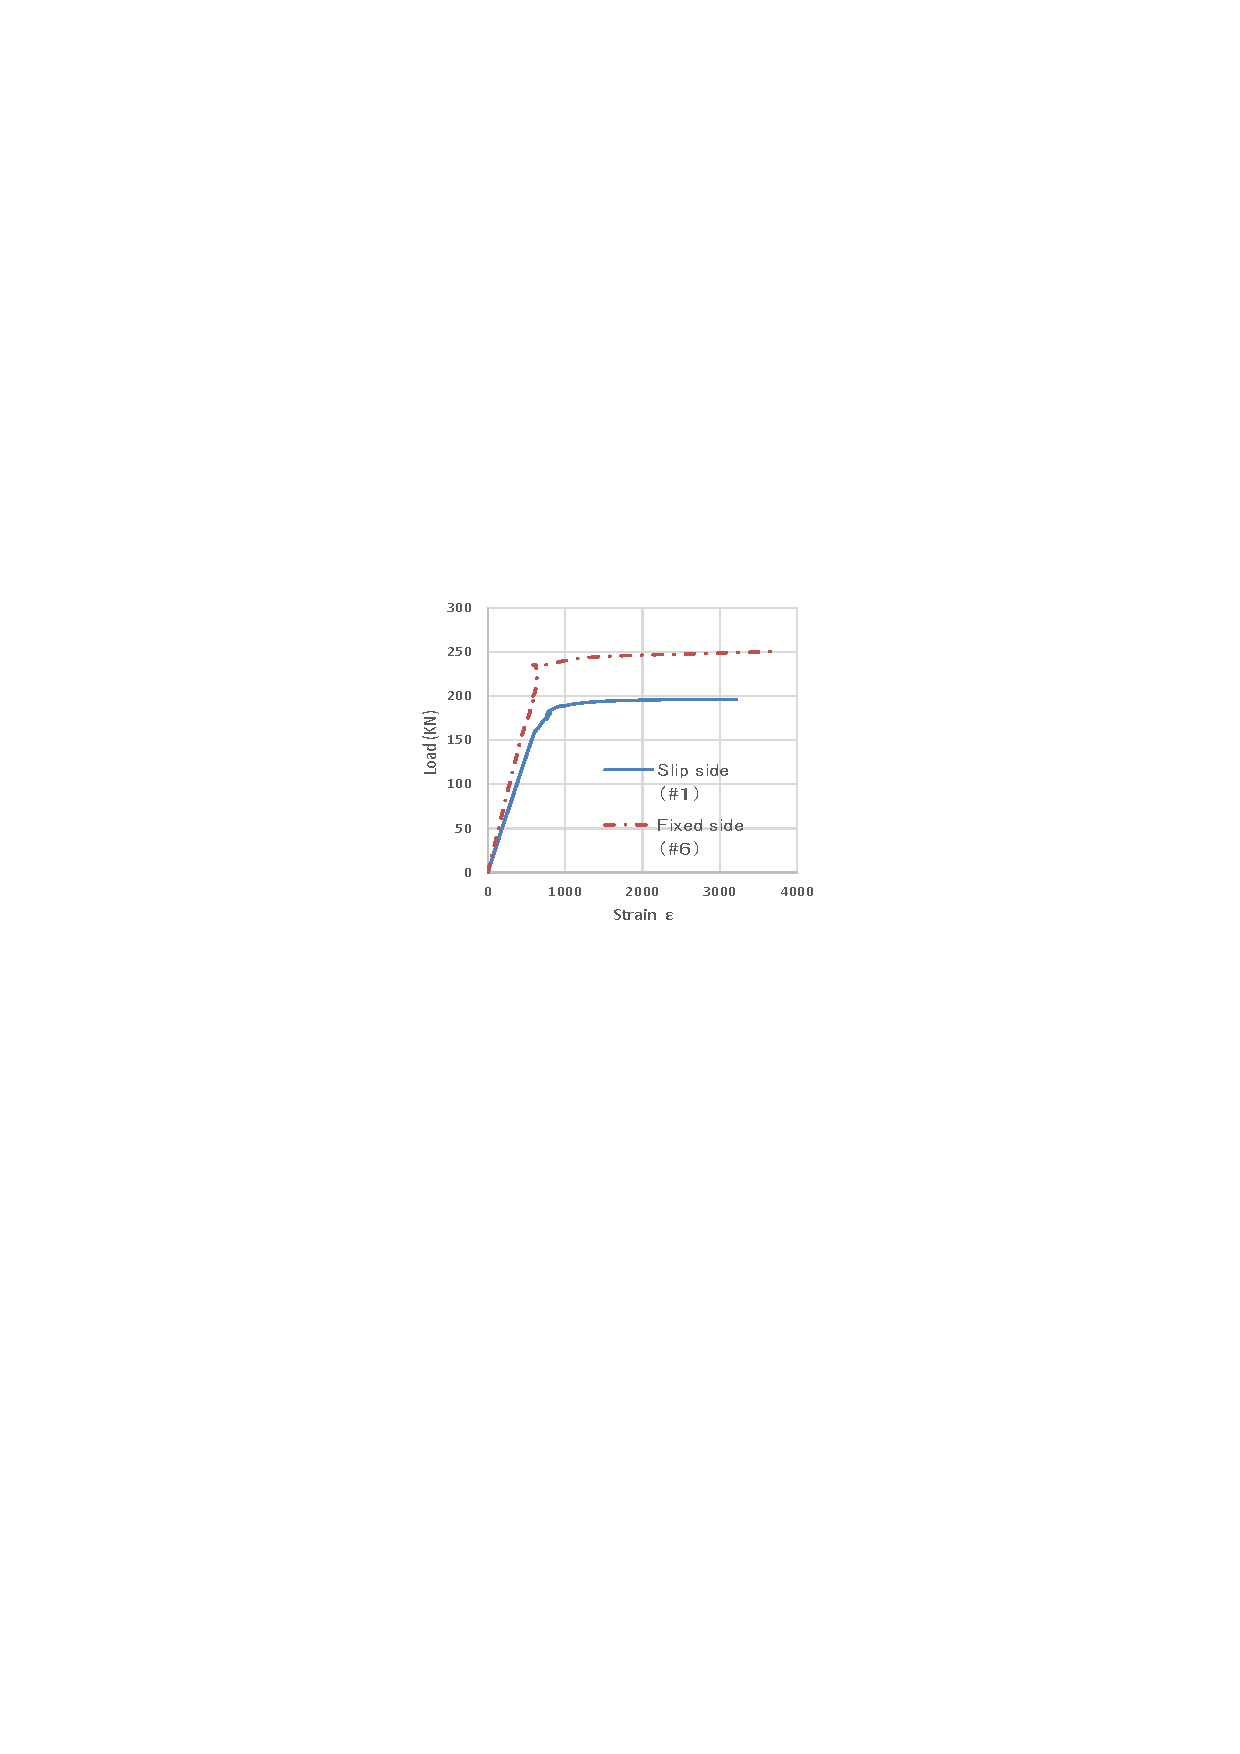
\includegraphics[width=\linewidth]{imgs/ch3/fig3-16.pdf}
    \caption{The relationship between Load and Strain, Net cross-section position (Hole \#1 and \#6)}
    \label{fig3-16}
    \end{minipage}
    \begin{minipage}[t]{0.48\textwidth}
    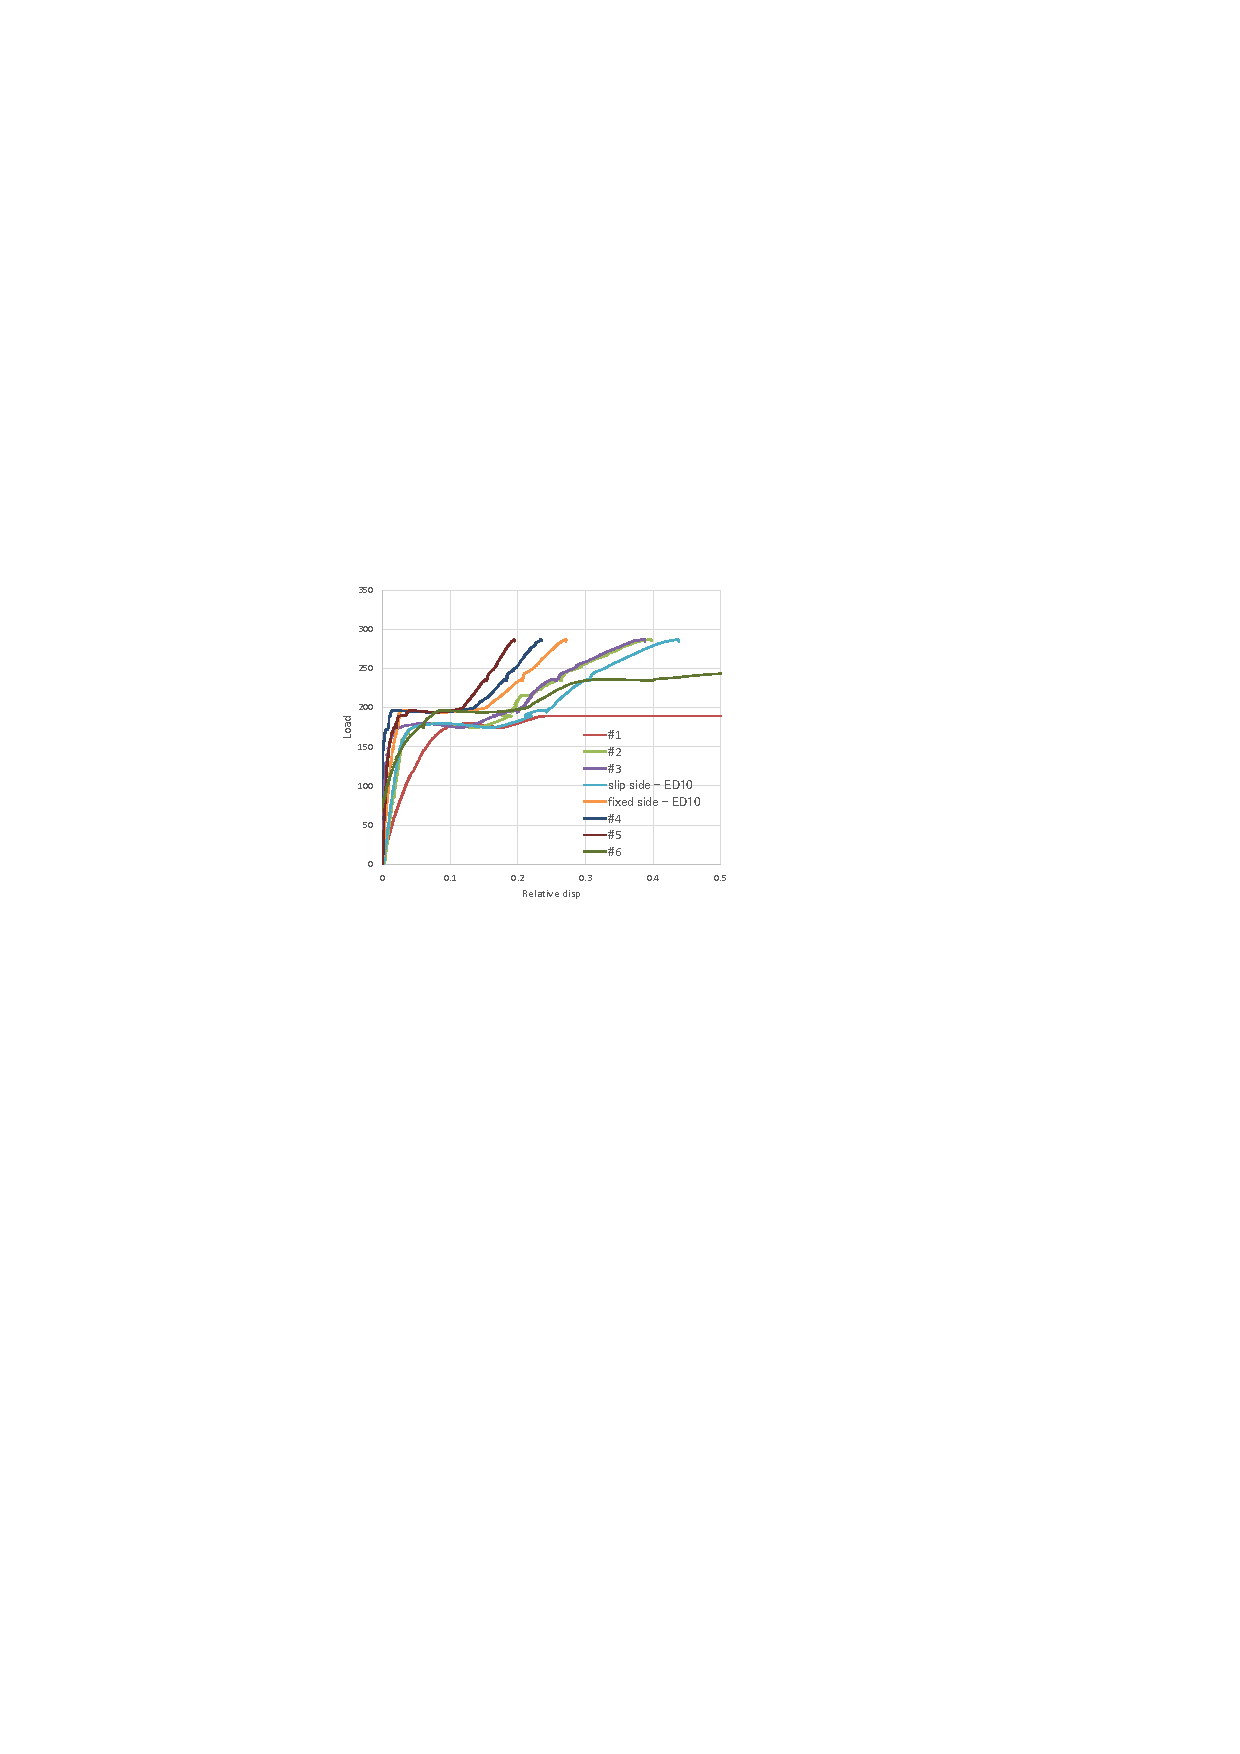
\includegraphics[width=\linewidth]{imgs/ch3/fig3-17.pdf}
    \caption{The relationship between Load and Displacement, each rivet position}
    \label{fig3-17}
    \end{minipage}
\end{figure}


When the rivets were sound, the maximum ultimate load was 286.7KN, which was 88\% of the calculated net section tensile strength (324.3KN). This is considered to be due to stress concentration near the rivet holes.

\begin{figure}[htbp]
    \centering
    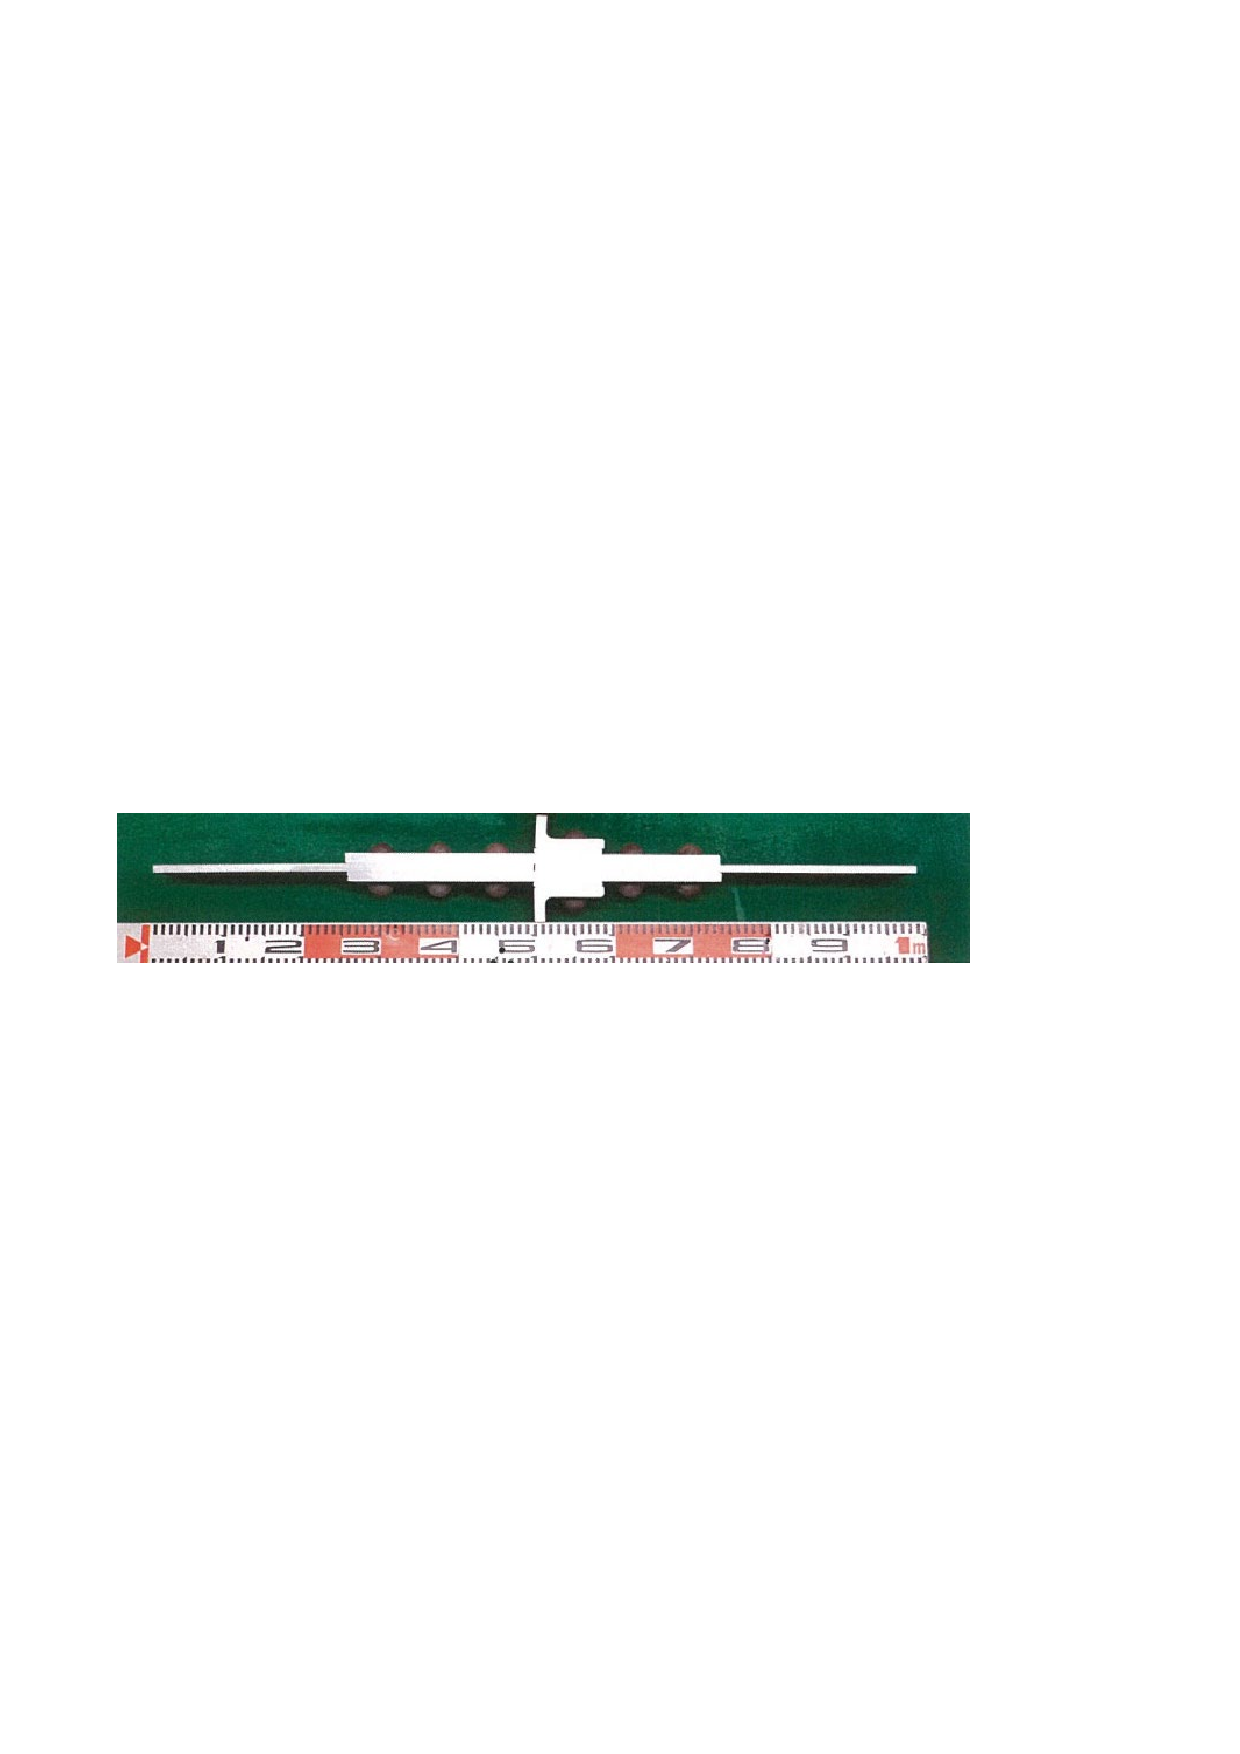
\includegraphics[width=0.7\textwidth]{imgs/ch3/fig3-18.pdf}
    \caption{Photograph of the riveted joint}
    \label{fig3-18}
\end{figure}


\subsubsection{RP1 case}

Fig.\ref{fig3-19} shows the strain relationship between the RP1 case load and the net cross-sectional position. Fig.\ref{fig3-20} shows the relationship between the load and the relative displacement of the main plate and the splice plate at 10 mm from the gap in the joint (End distance 10mm, ED-10) and each hole position.

The relative displacement of the fixed side (so-called "rivet soundness") was smaller than that of the sliding side. The first gradient was that the rivet deformed while the slip began to occur. The next change in slope was the rivet entering a bearing state, and the rivet bit into the bearing little by little.

The maximum tensile load on the joint cannot be shown in the graph because the CDP displacement transducer could not follow the plastic displacement, but based on Amsler's maximum load reading, the maximum load is 304.4KN. This is 95.5\% of the net section tensile load of the steel (318.8KN). The fact that the maximum load was about 95.5\% of the steel's tensile capacity can be attributed to the load transfer to the splice plate due to the clamping force of the high-strength bolt and the relaxation of stress concentration caused by the cross-sectional deficiency near the bolt holes.

The calculated net sectional yield capacity of the RP1 case was 193.3KN (enlarged hole), and actually 216.2KN when the net sectional yield occurred near the bolt hole. This is about 12\% higher than the design value, which is also the result of the load transfer by the frictional force of the outer bolt before.

\begin{figure}[htbp]
    \centering
    \begin{minipage}[t]{0.48\textwidth}
    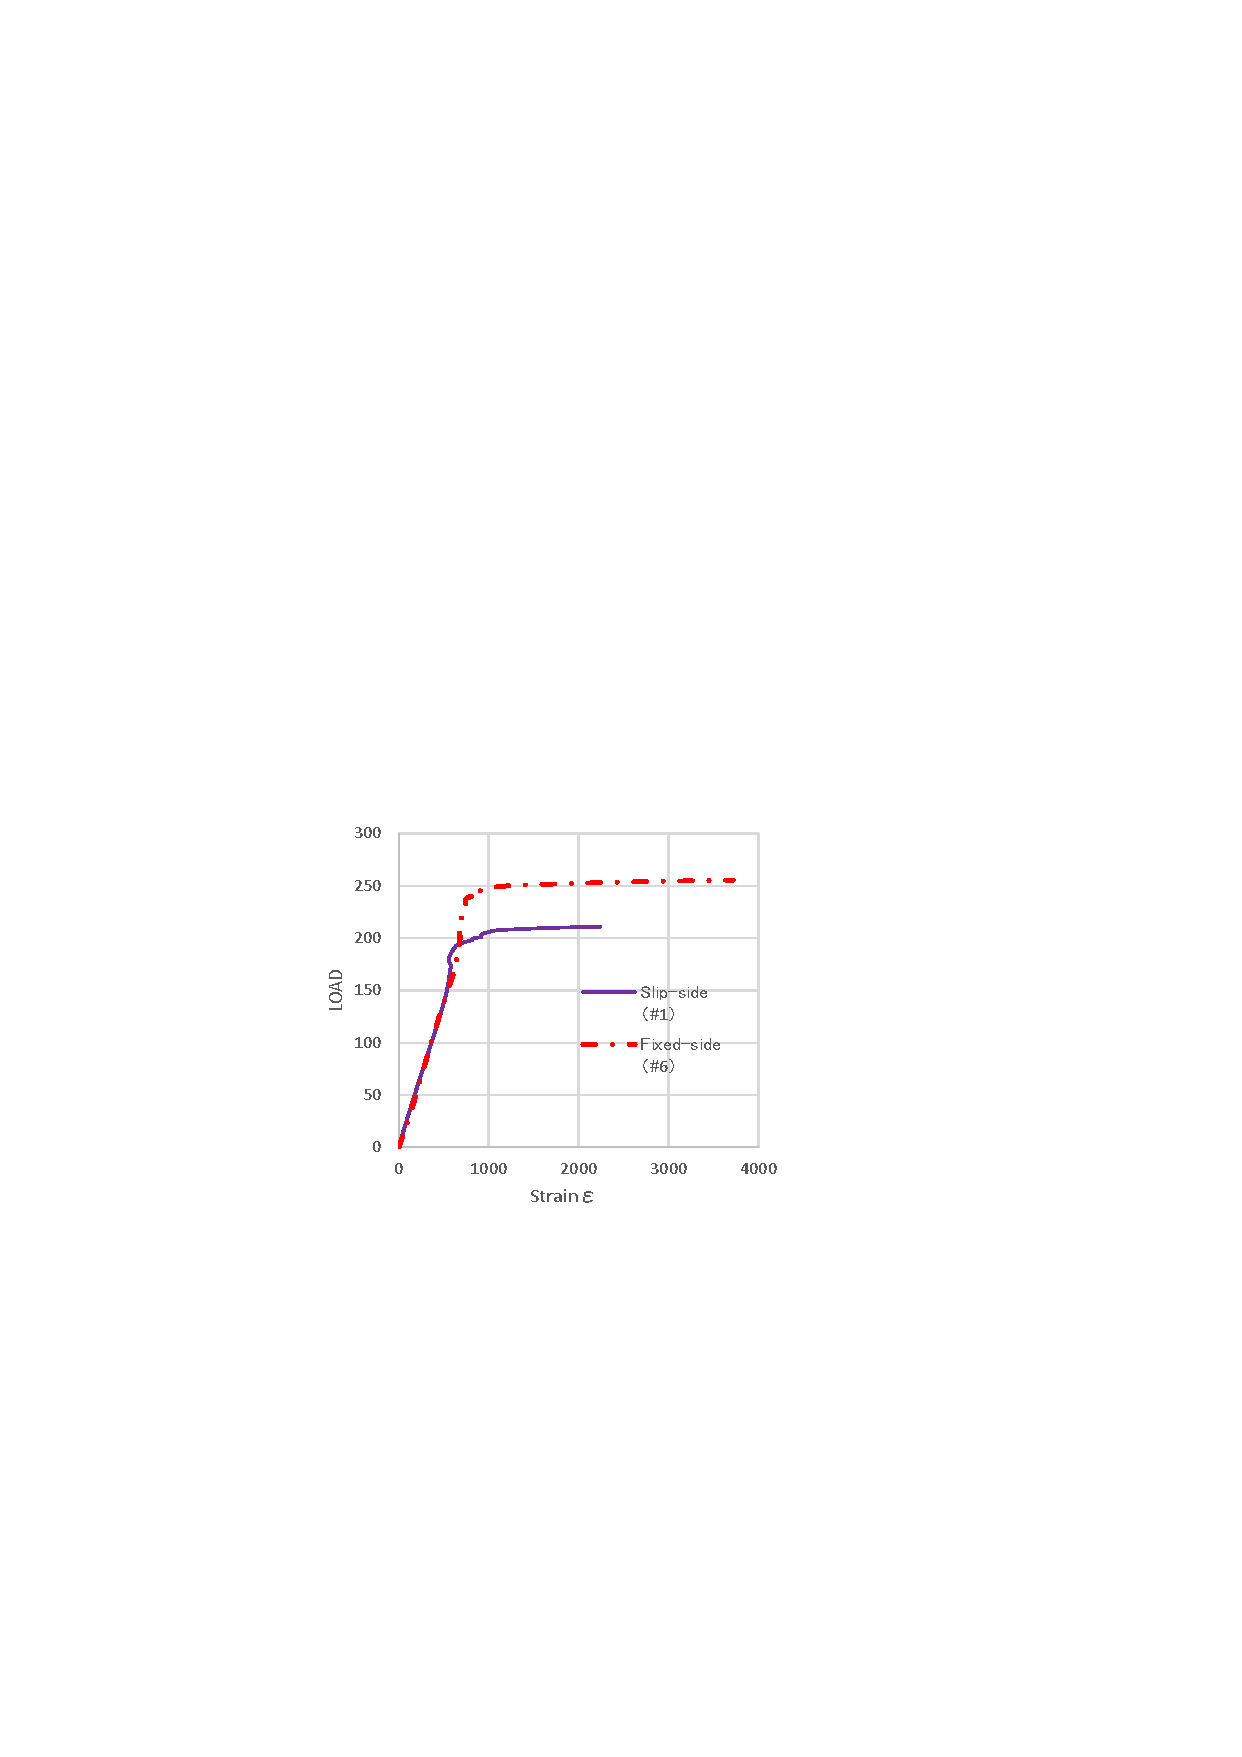
\includegraphics[width=\linewidth]{imgs/ch3/fig3-19.pdf}
    \caption{The relationship between Load and Strain, Net cross-section position (Hole \#1 and \#6)}
    \label{fig3-19}
    \end{minipage}
    \begin{minipage}[t]{0.48\textwidth}
    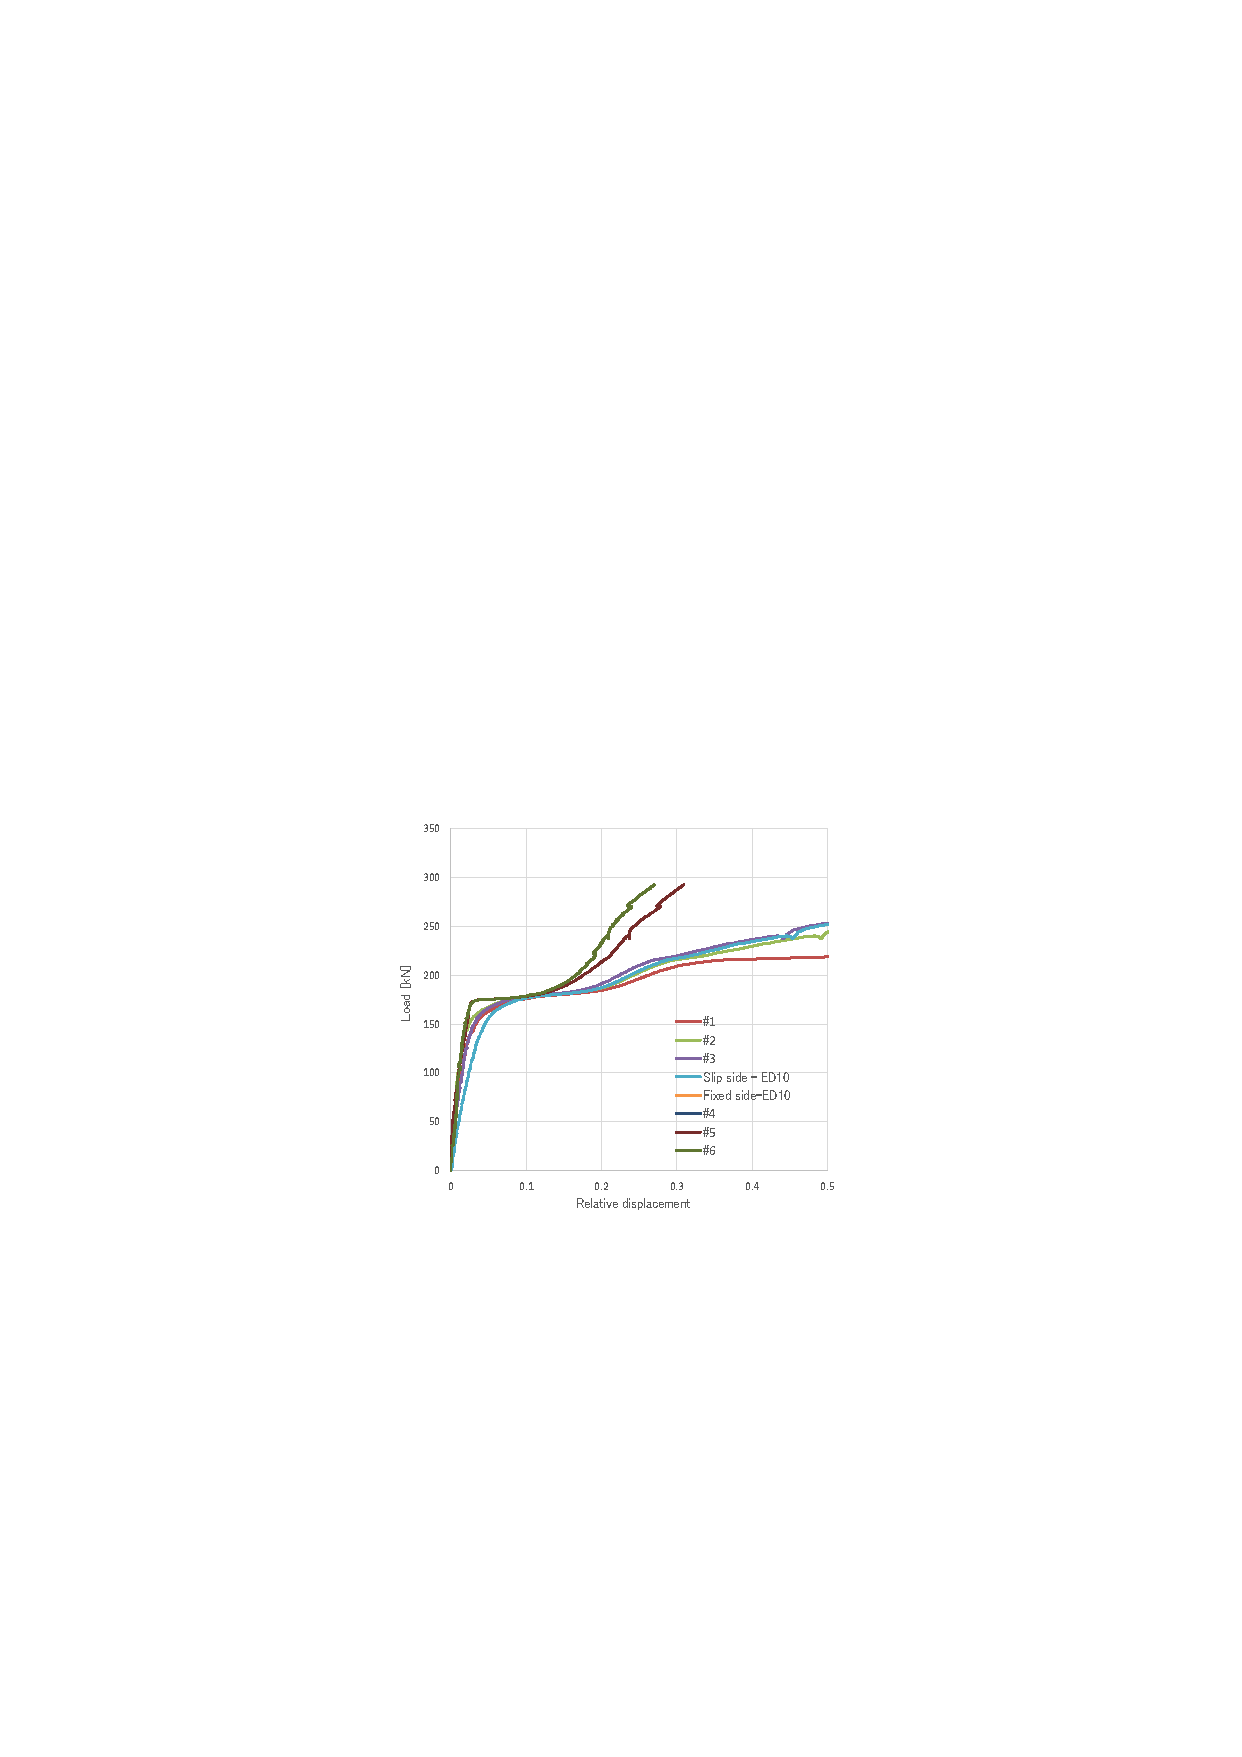
\includegraphics[width=\linewidth]{imgs/ch3/fig3-20.pdf}
    \caption{The relationship between Load and Displacement of RP1 Case, each rivet position}
    \label{fig3-20}
    \end{minipage}
\end{figure} 

\subsubsection{RPALL case}

In the RPALL case, the rivets were removed from the entire joint, the rivet holes were enlarged, and replaced with M22F10T high-strength bolts. The order of rivet replacement was \#1, \#6, \#2, \#5, \#3, and \#4 according to the recommended order for replacing three rows of rivets in the literature by Kakimoto et al.14, taking the rivet bearing force into consideration. (The bottle order was set from the edge end of one side of the joint to the edge end of the other side of the joint.)
Fig.\ref{fig3-21} shows the RPALL case load-strain relationship at the net cross-sectional location. The tensile side of the RPALL had a friction coefficient of 0.21, and the M22F10T introduced average axial force was 215.5KN and slip load was 271.5 kN.
The tensile load-relative displacement relationship is shown in Figure 3.22. The load was 271KN when the relative displacement was 0.2mm. This is almost the same as the calculated slip load using the slip coefficient obtained from the results of the small-slip test.
As shown in Fig.\ref{fig3-21}, the net sectional yield capacity of the RPALL was 207KN, which was about 1.09 times higher than the calculated net sectional yield value (190 kN). This is considered to be due to load transfer to the splice plate by the clamping force. Finally, the maximum load of RPALL was 293KN, which is about 0.93 times higher than the design net section tensile load of 315 kN, 5\% higher than the RivetCase but 2\% lower than the RP1Case. The friction force of the outer bolt of RP1 was 1.3\% greater than that of RPALL, and the load was transferred by the edge of the bolt due to the friction force.

\begin{figure}[htbp]
    \centering
    \begin{minipage}[t]{0.48\textwidth}
    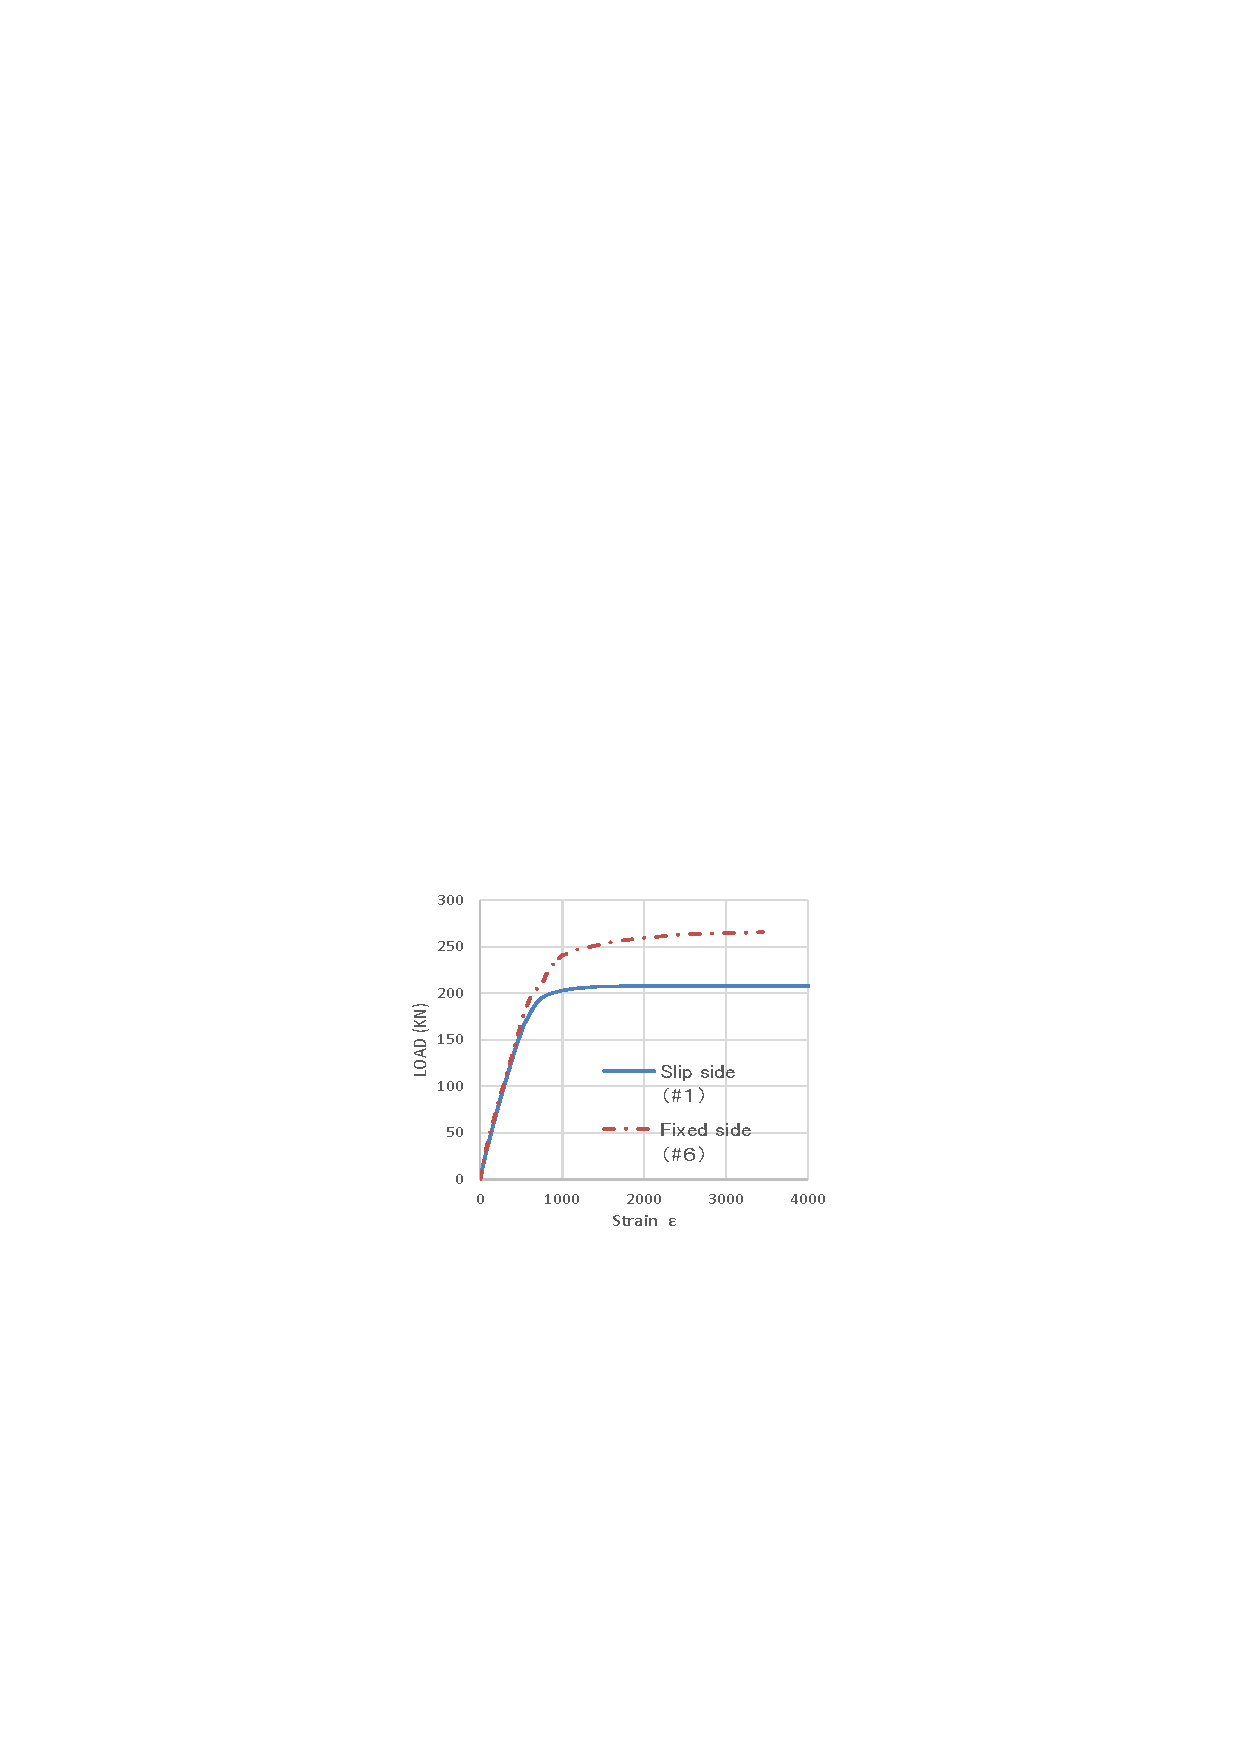
\includegraphics[width=\linewidth]{imgs/ch3/fig3-21.pdf}
    \caption{The relationship between Load and Strain, Net cross-section position (Hole \#1 and \#6)}
    \label{fig3-21}
    \end{minipage}
    \begin{minipage}[t]{0.48\textwidth}
    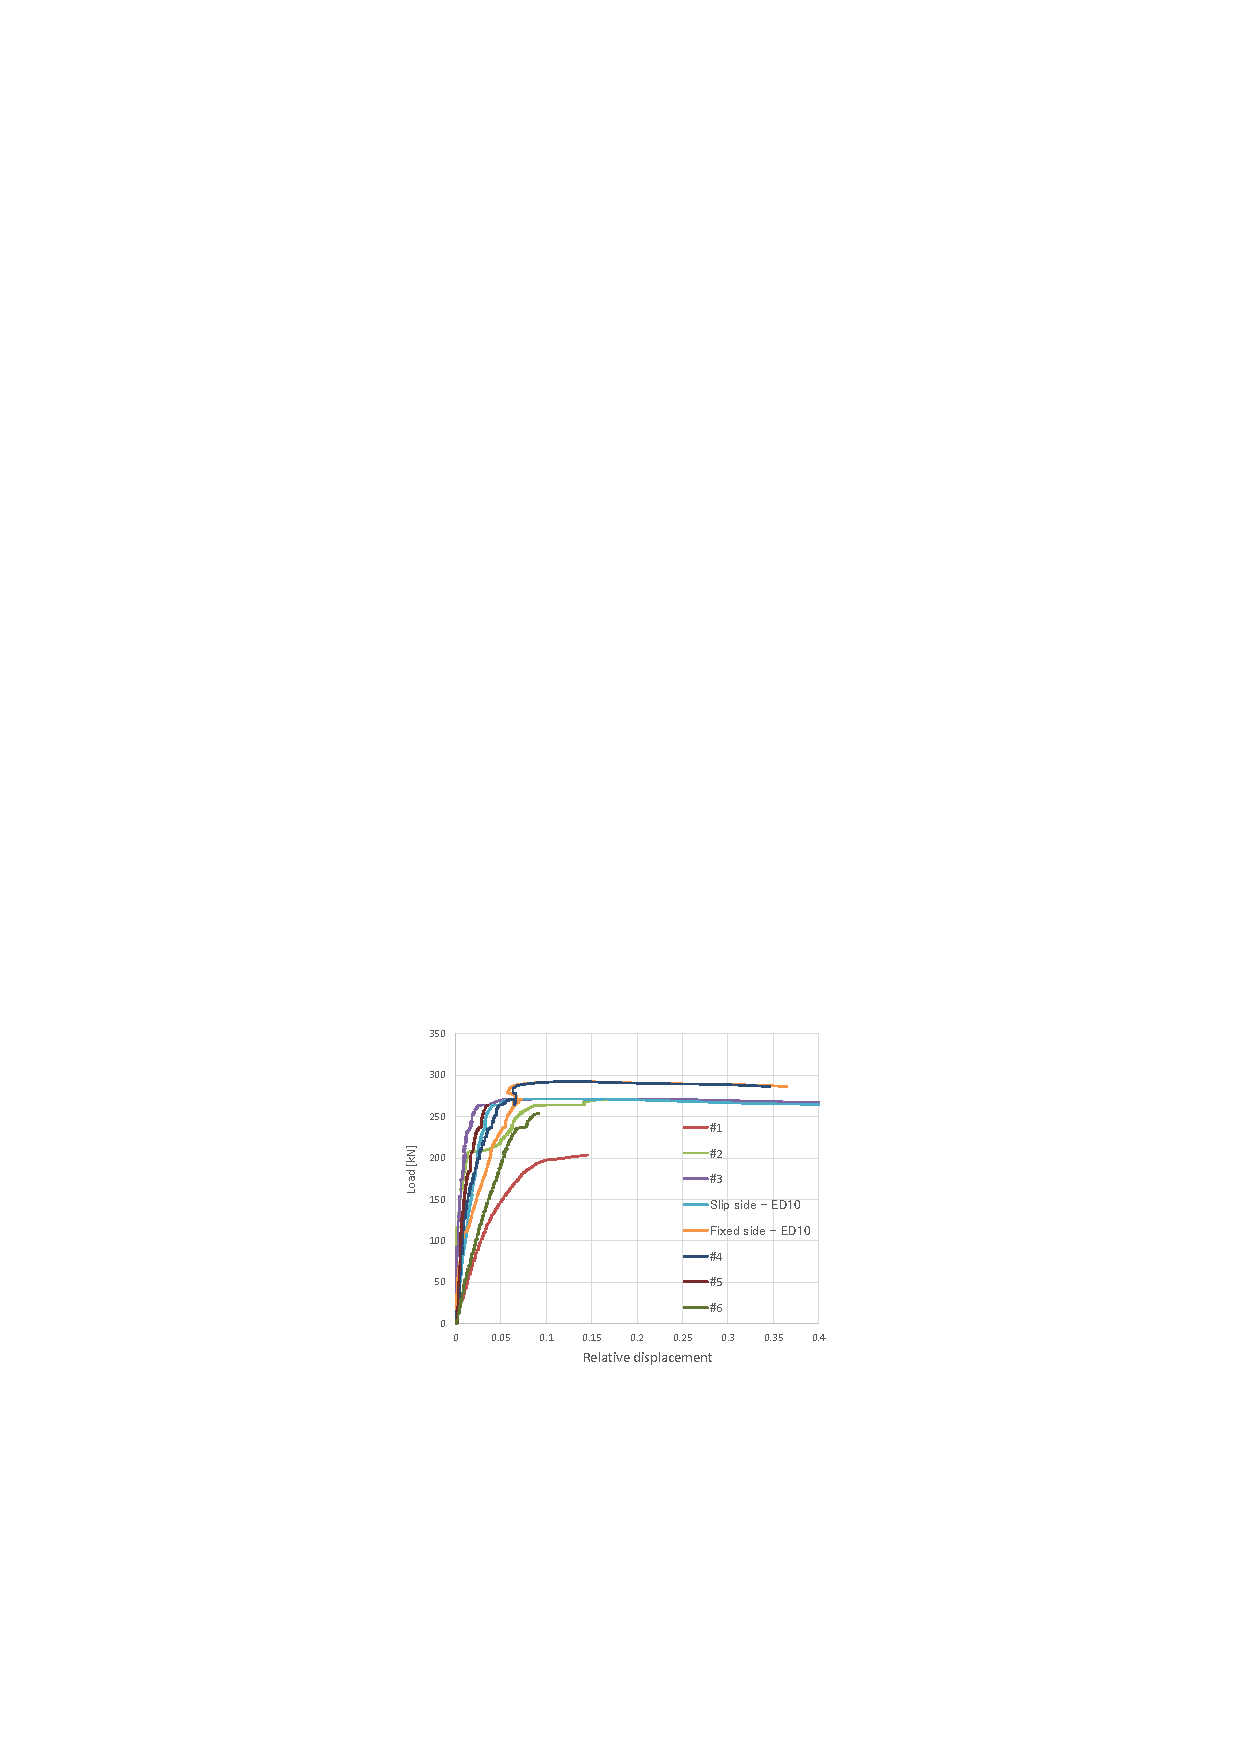
\includegraphics[width=\linewidth]{imgs/ch3/fig3-22.pdf}
    \caption{The relationship between Load and Displacement of RPALL Case, each rivet position}
    \label{fig3-22}
    \end{minipage}
\end{figure} 

\subsection{Load sharing of each case}

Fig.\ref{fig3-23} compares the maximum load in each case with the yield capacity and tensile capacity of each case. The test specimens were cut from actual girders, and the dimensions of each case were slightly different.

The maximum load in the sound condition was 1.45 compared to the yield capacity, while the maximum loads of RP1 and RP2 were 1.53 and 1.52, respectively, both slightly higher than that of RPALL. Kobayashi et al. \cite{KOMATSU2015} showed that replacing friction high-strength bolts slightly increased the bearing capacity of joints determined by pure sectional yield, but this study further examined a partial replacement repair plan (replacing high-strength bolts only on the outside). As a result, the bearing capacity of the three-row joint was almost the same by replacing only the outer joint with a high-strength bolt as in the case where the entire joint was replaced with a high-strength bolt, suggesting that the partial replacement repair (so-called combined joint of friction high-strength bolt and bearing rivet) is effective.

Fig.\ref{fig3-24}.a show the strain in the joint's main plate when the load is 60\% of the design yield capacity. In this experiment, a total of seven strain gauges were attached at equal intervals from the splice plate to the play area, where T2, T4, and T6 are the positions of the rivet holes. The stress concentration around the bolt holes in the main plate was relieved by the frictional force that was generated and transmitted to the splice plate. In the other cases (RP2 and RP3), the strain in the main plate shows a similar trend, with a convexity in the strain near the pure section of the main plate, and unlike RP1 and RPALL, the strain does not decrease much after the load passes through the hole. This is thought to indicate that the load is not transferred to the splice plate very well.

Fig.\ref{fig3-24}.b shows the distribution of main plate strain at net section yield ($P/P_y=1$) for each case design. The joints in the sound condition first entered the net section yielding state, and high stress concentrations also occurred near the net section in the RP2 and RP3 cases, which is especially noticeable in RP3 (where the bolt displaces the inside of the joint). RPALL and RP1 also showed the same trend, with a small amount of convexity also starting to appear near the pure section.

\begin{figure}[htbp]
    \centering
    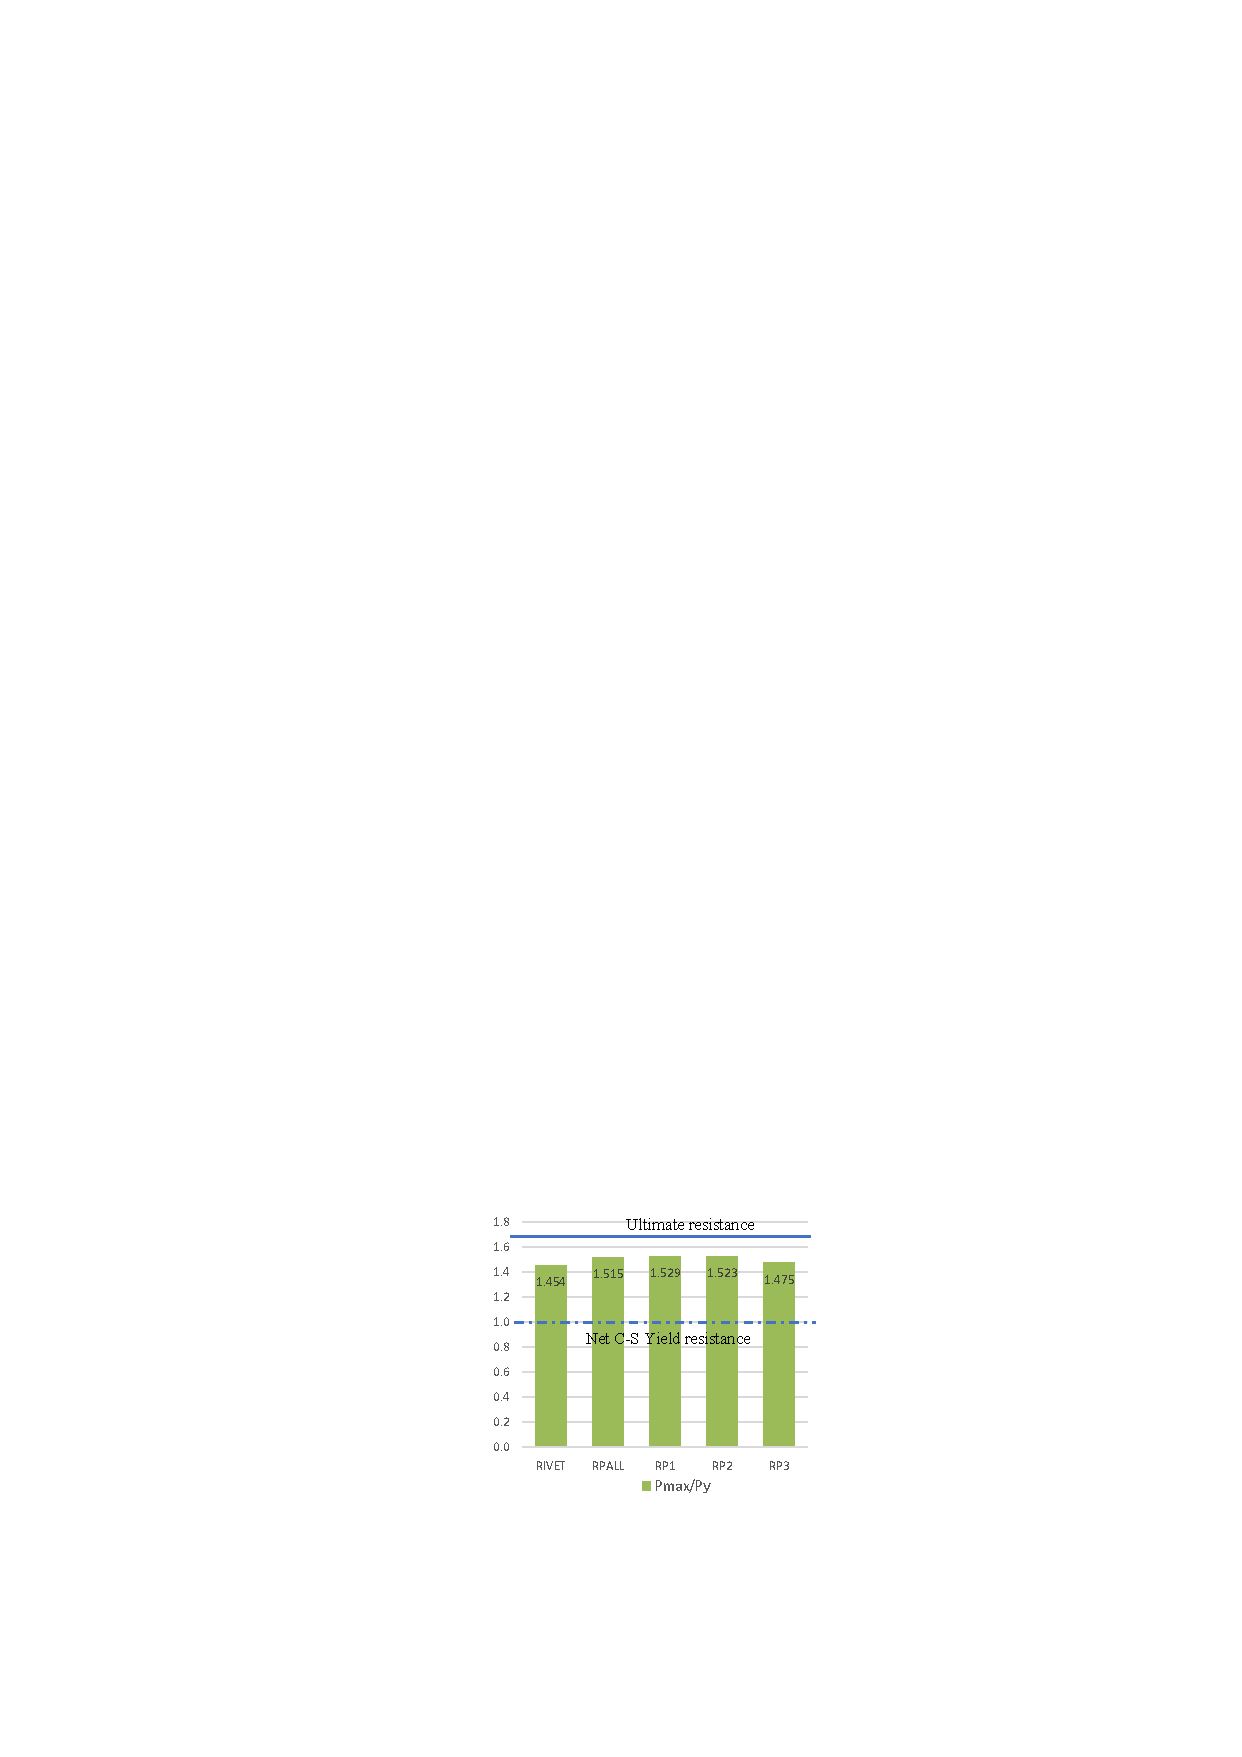
\includegraphics[width=0.6\textwidth]{imgs/ch3/fig3-23.pdf}
    \caption{Comparison of the maximum load in each case with the yield capacity and tensile capacity of each case}
    \label{fig3-23}
\end{figure}

\begin{figure}[htbp]
    \centering
    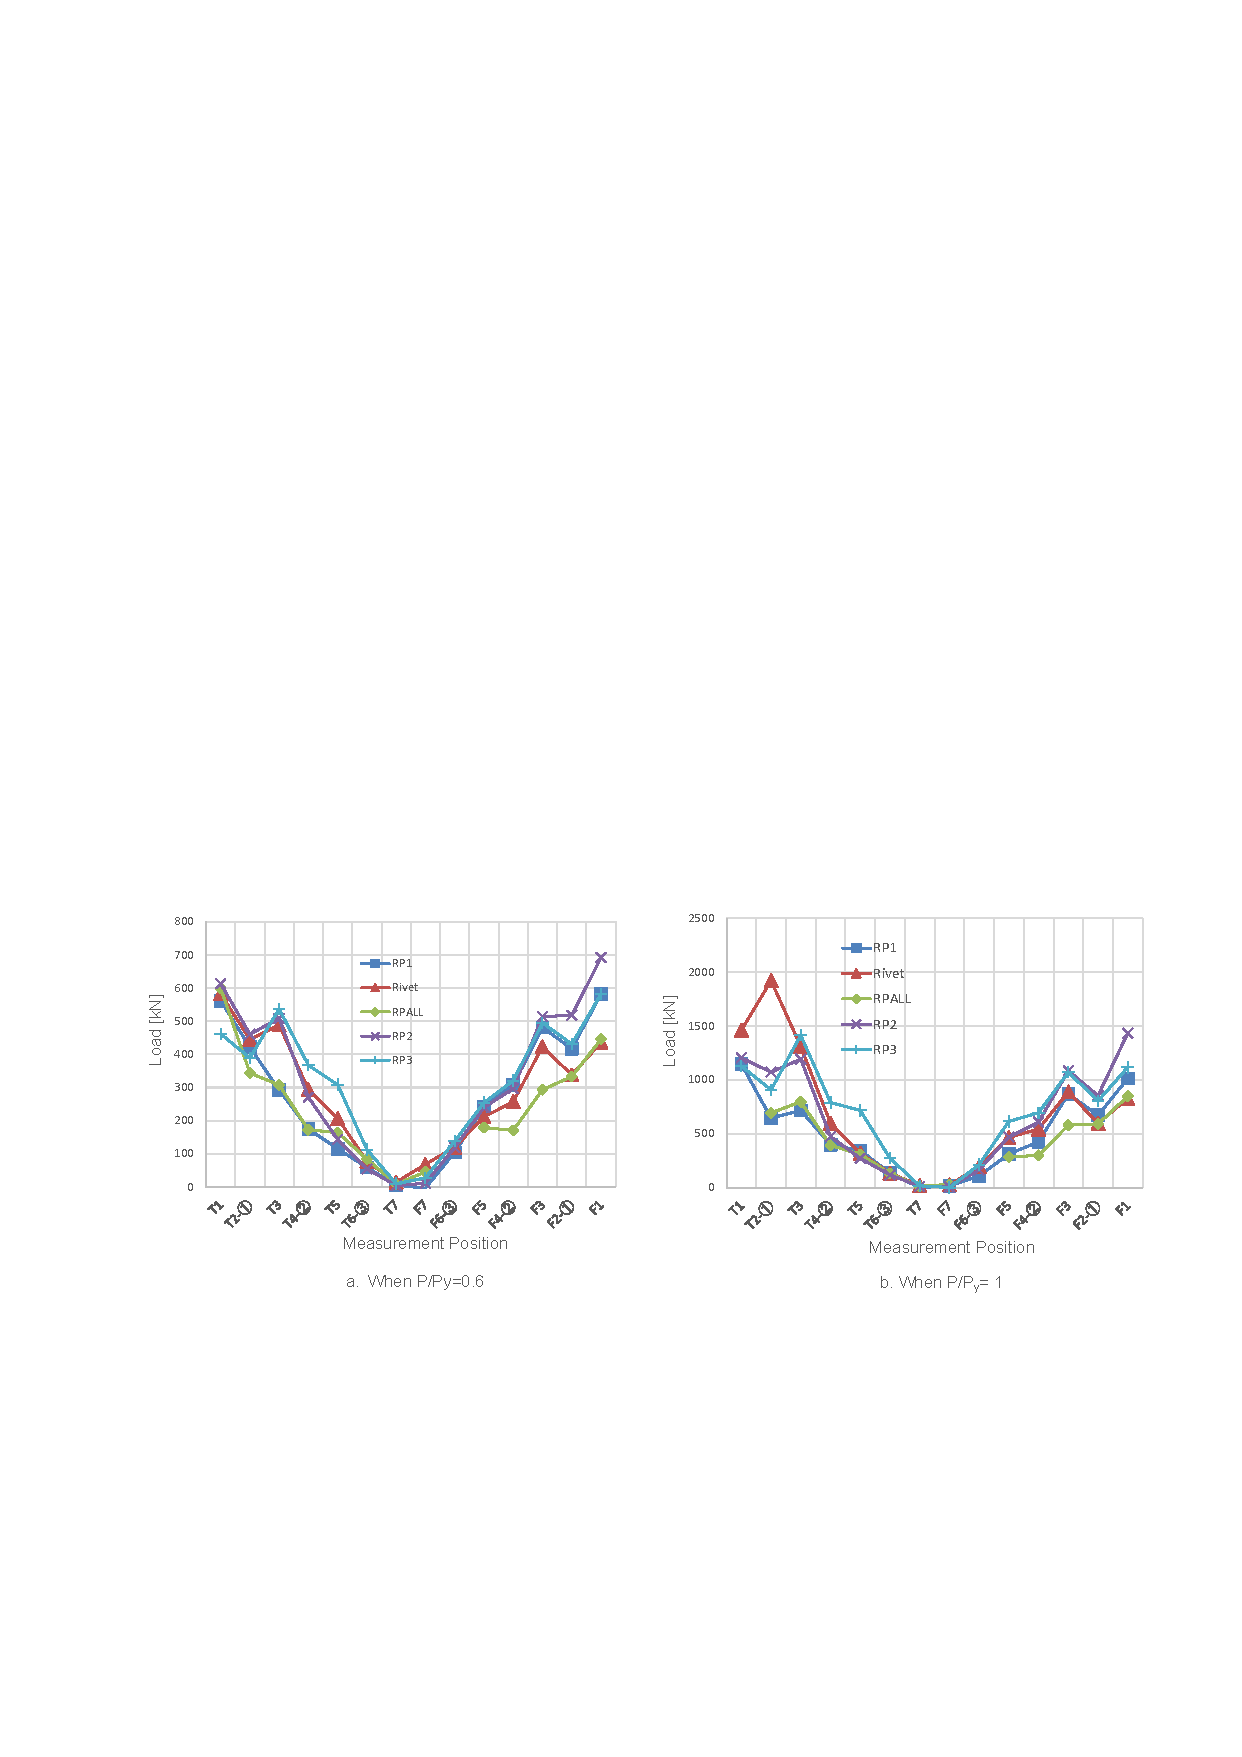
\includegraphics[width=0.9\textwidth]{imgs/ch3/fig3-24.pdf}
    \caption{the strain distribution in the joint's main plate}
    \label{fig3-24}
\end{figure}


The load transfer coefficient to the main plate at the joint is shown in Fig.\ref{fig3-26}.a P/Py=0.6 and b. P/Py=1 show the load transfer coefficient when the load is 0.6 and 1 times the quasi-sectional yield capacity of the joint, respectively. The Rivet case shows that the load transfer coefficient of T3 after rivet 1 is 74\% and the cross-sectional area ratio of the joint main plate is 72\%, which is almost the same as that of the Rivet case.

\begin{figure}[htbp]
    \centering
    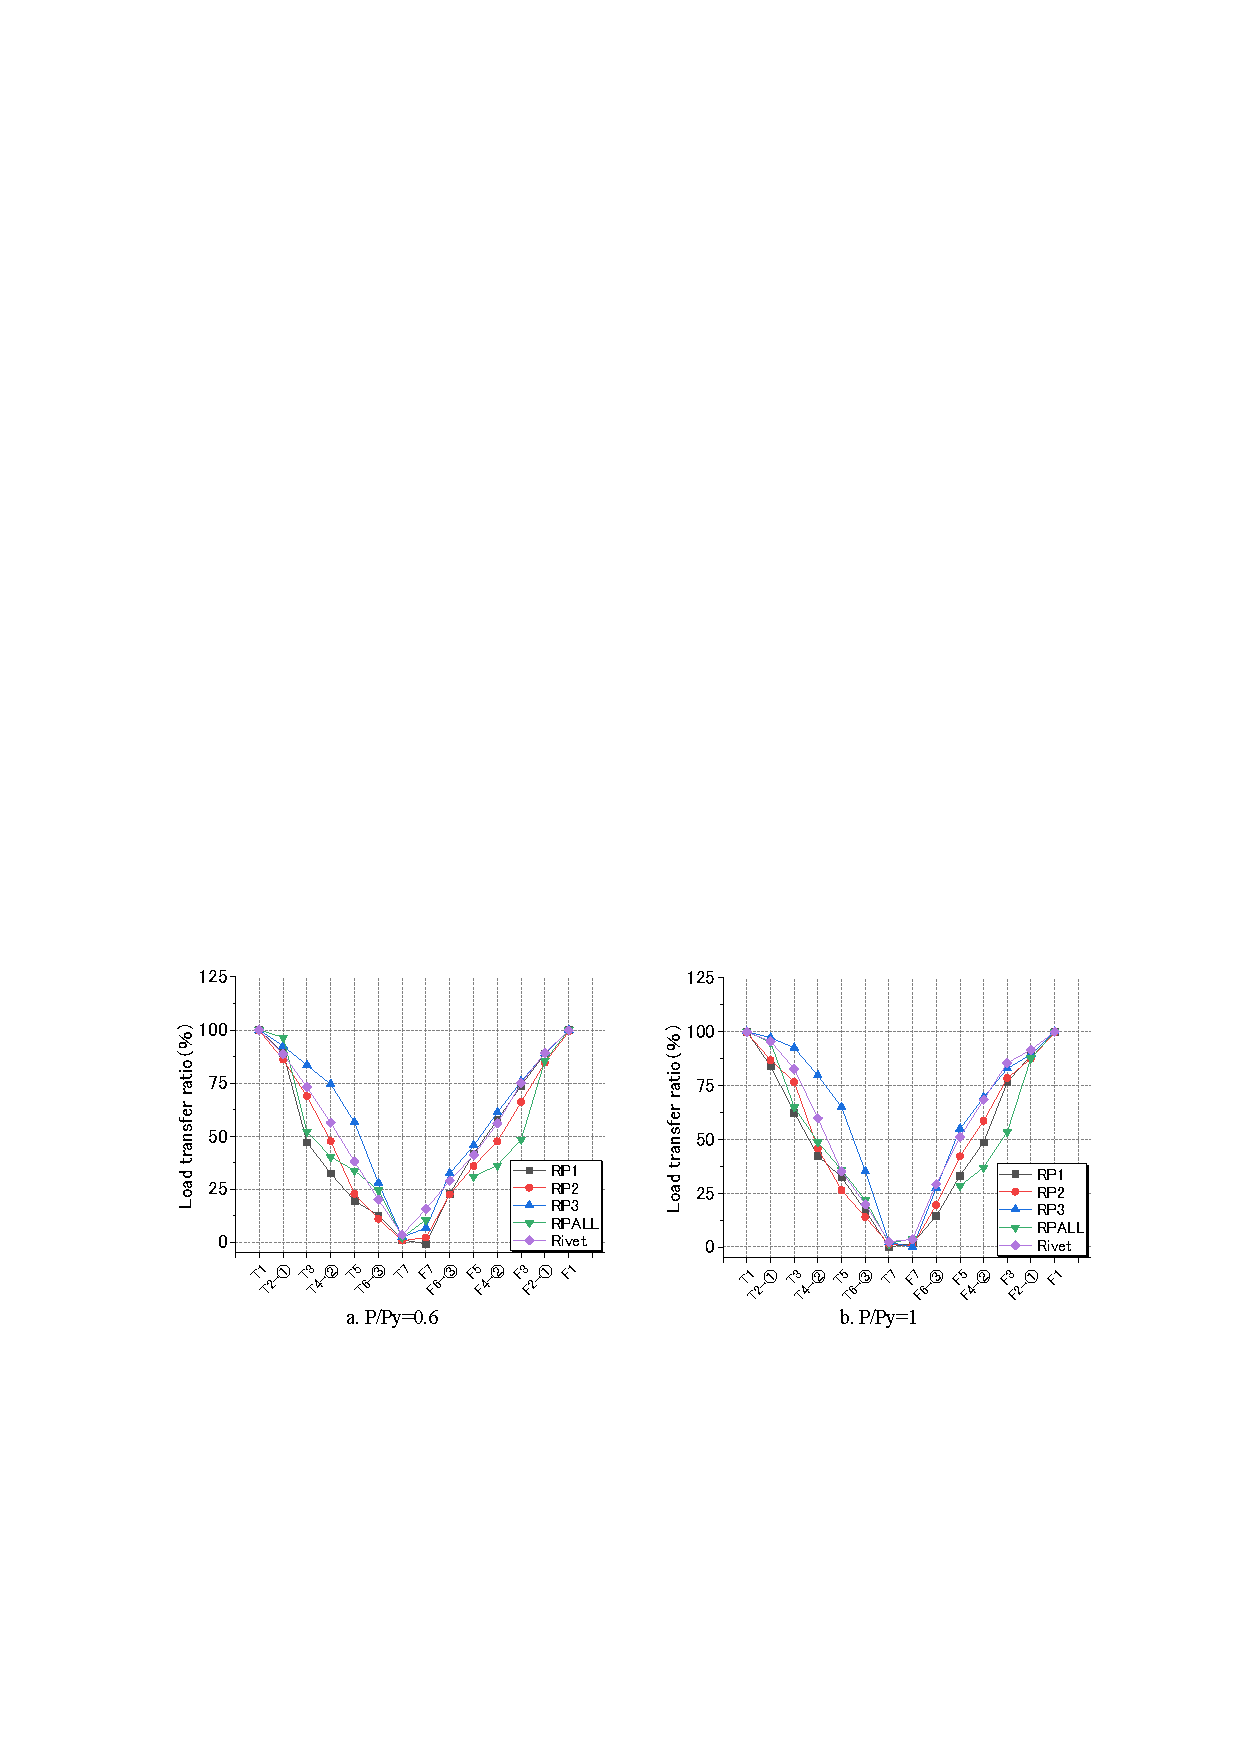
\includegraphics[width=0.9\textwidth]{imgs/ch3/fig3-26.pdf}
    \caption{the load transfer ratio to the main plate at the joint}
    \label{fig3-26}
\end{figure}


\subsection{Overvation of the faying surface}

The ruptured RPALL (high-strength bolt all replaced) specimen was disassembled and the cross section was observed. A photograph of the contact surface is shown in Fig.\ref{fig3-27}. The results of the small-slip test described in the previous section show that the slip coefficients of the two splice plates in contact with the main plate are different from each other, and there is a large difference between the slip coefficients of the fixed side and the sliding side. Fig.\ref{fig3-28} shows the difference in the slip coefficients between the fixed and sliding sides, the fixed side exhibited slip on only one side, which was attributed to the large difference in the coefficient of friction between the two contacting surfaces. Fig.\ref{fig3-29} and Fig.\ref{fig3-30} show enlarged views of the tensile and anchorage sides, respectively. Observation of the contact surface on the fixed side shown in Figure 3.30 confirms that slip occurred on only one side. Slip on the fixed side was considered to have occurred after yielding and before the slip on the sliding side occurred. The small-slip test showed that the coefficient of slip on the surface of the fixed side of the joint averaged 0.35, while the coefficient of slip on the opposite side averaged only 0.16. Although the same main plate was used, the difference between the coefficients of slip on the surface and the back was approximately twice that of the fixed side.

In the future, when repairing and reinforcing aged riveted bridges with friction high-strength bolts, sufficient attention should be paid to the difference in slip coefficients.

\begin{figure}[htbp]
    \centering
    \begin{minipage}[t]{0.45\textwidth}
    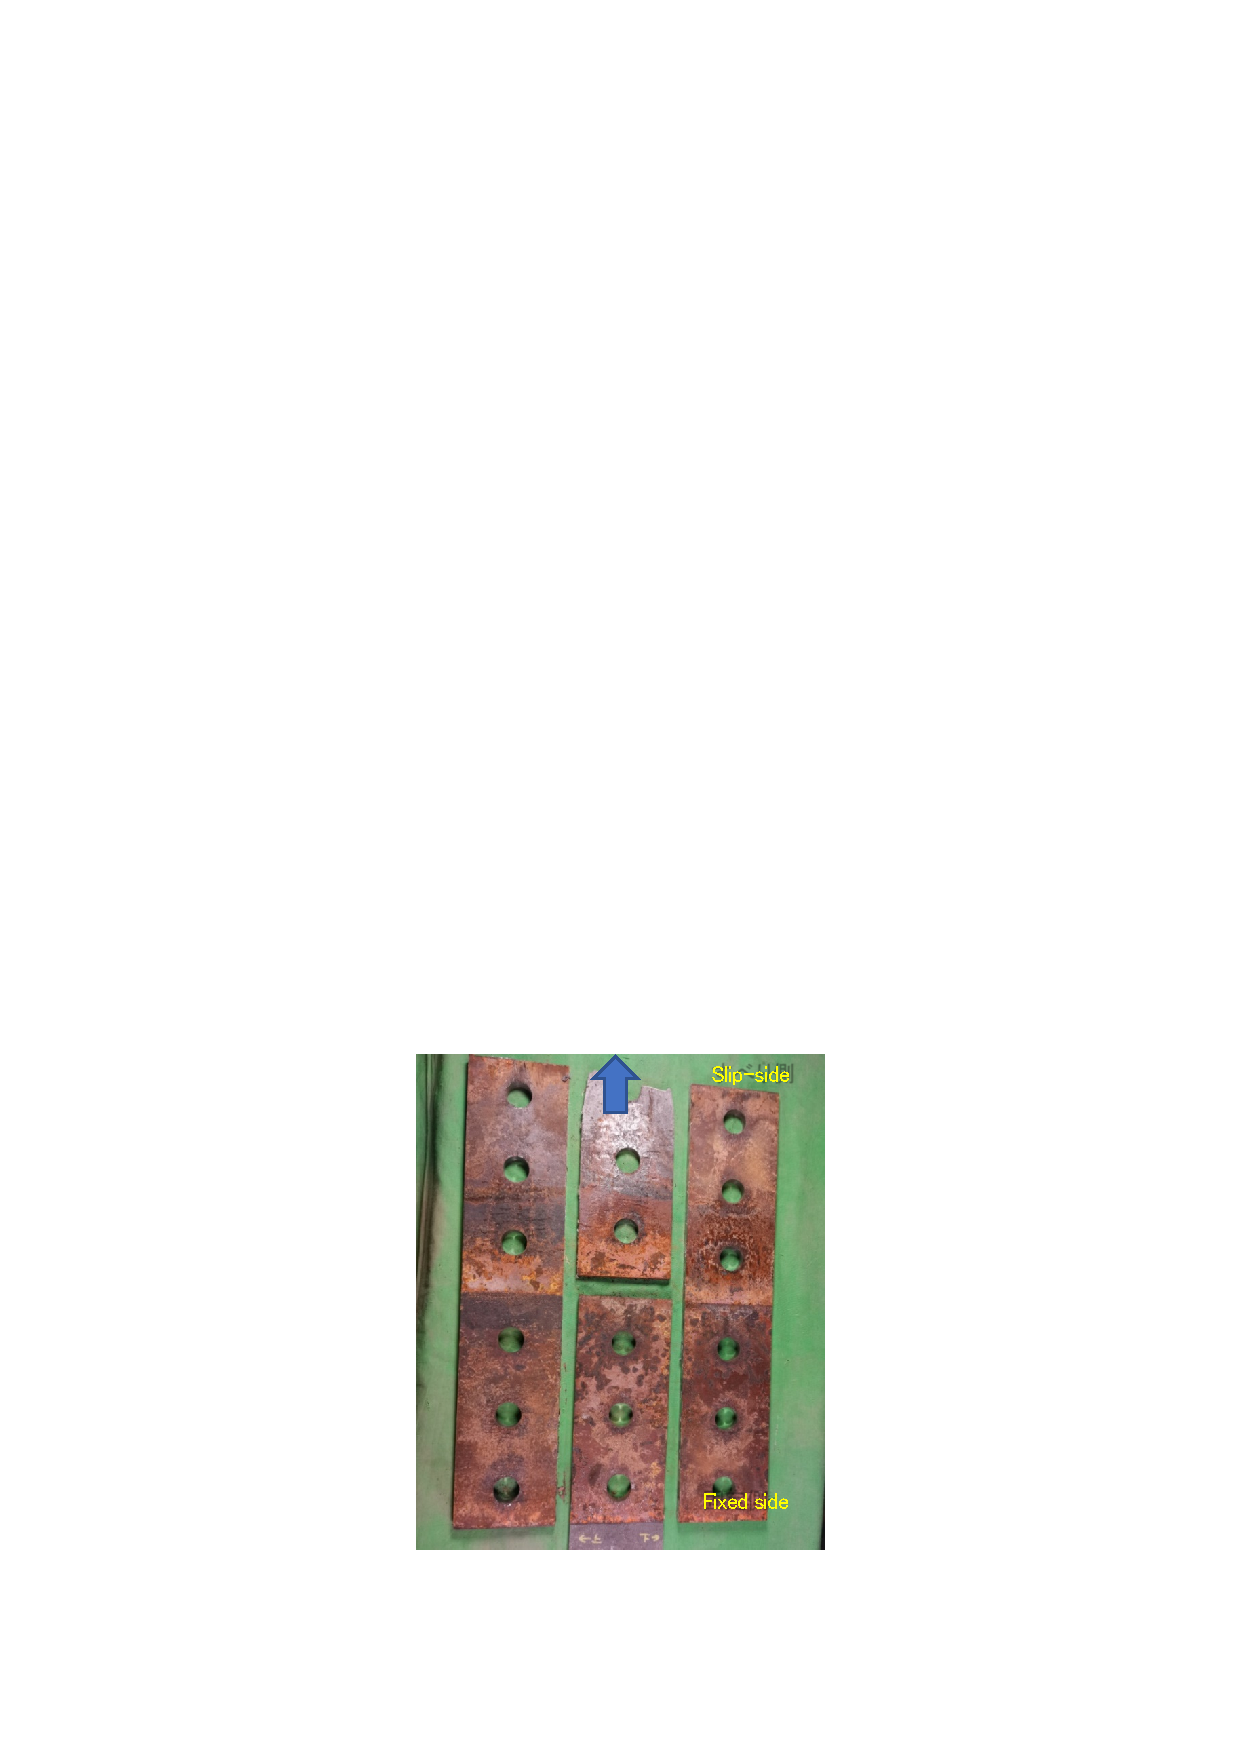
\includegraphics[width=\linewidth]{imgs/ch3/fig3-27.pdf}
    \caption{Photograph of the contact surface}
    \label{fig3-27}
    \end{minipage}
    \begin{minipage}[t]{0.3\textwidth}
    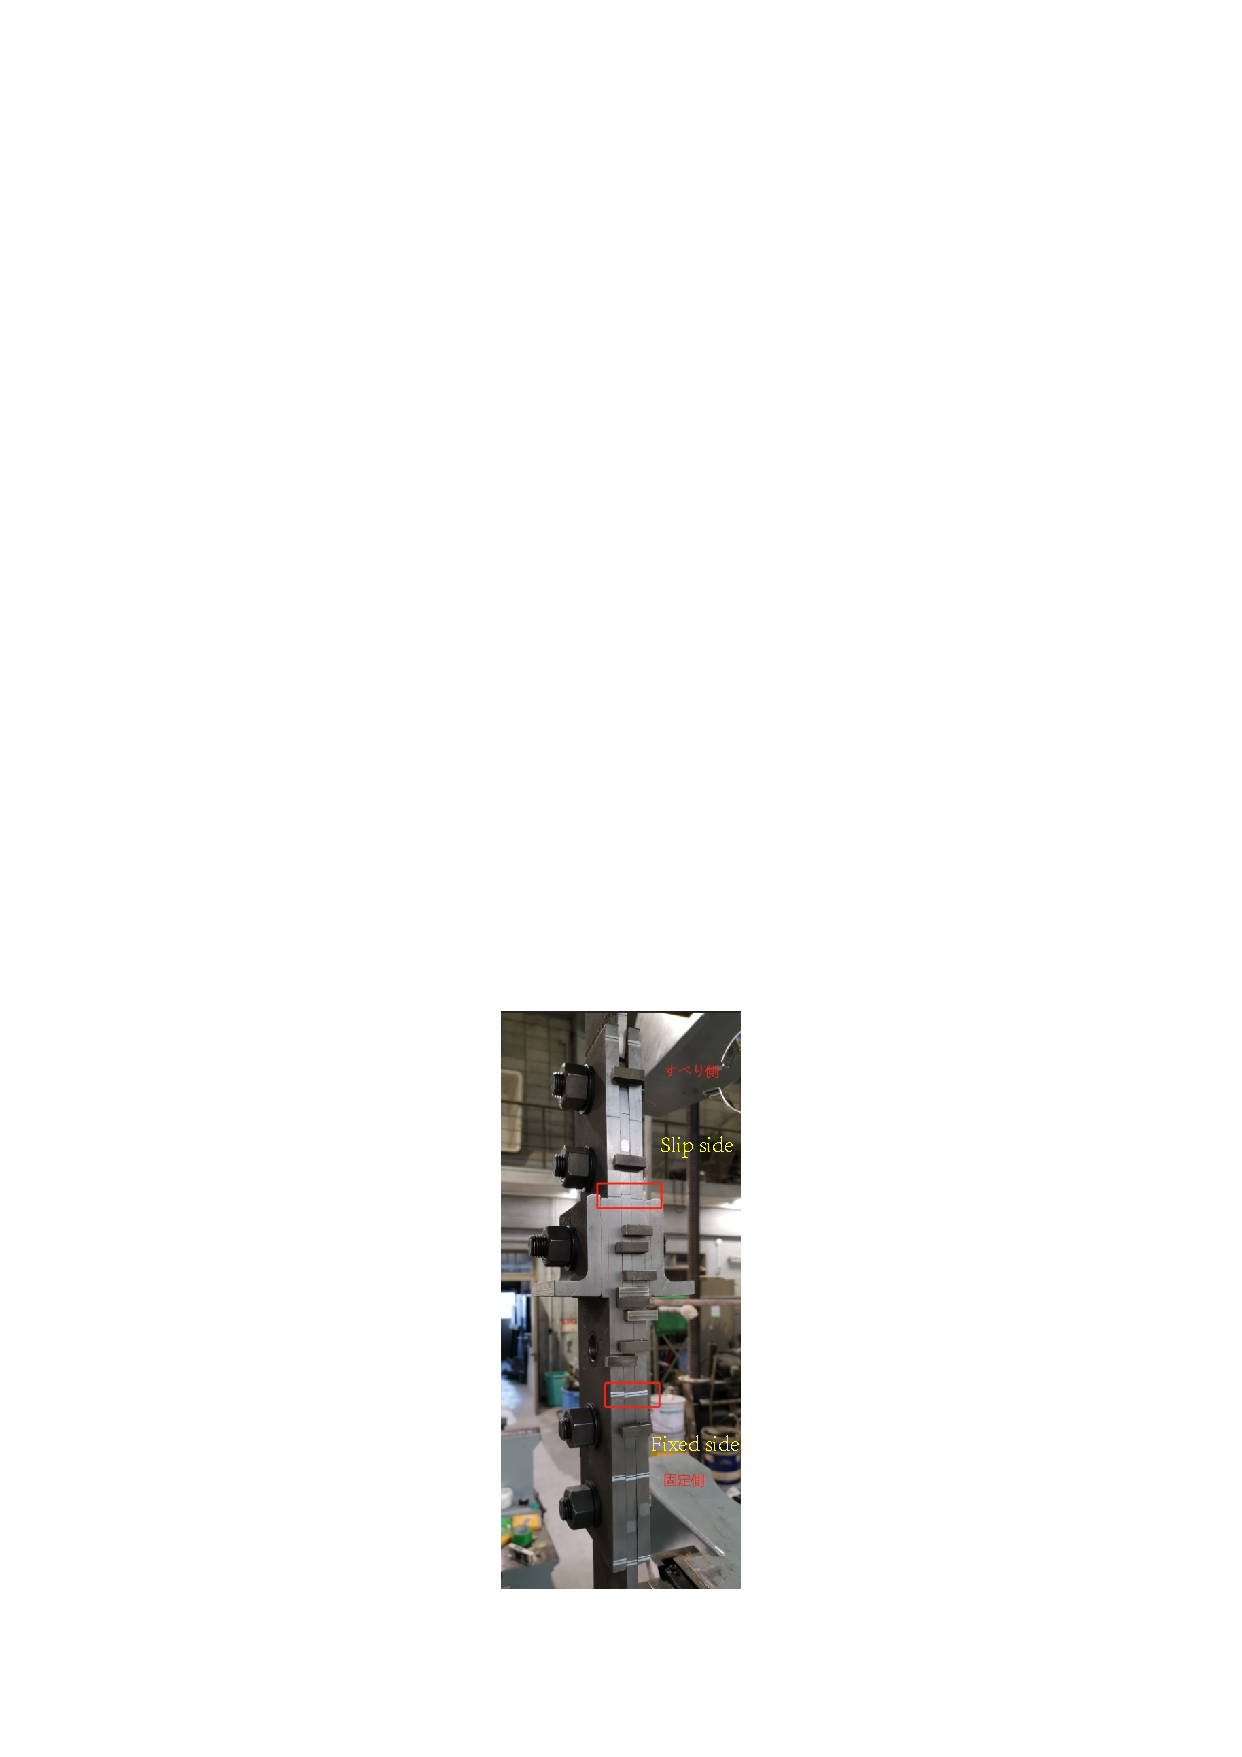
\includegraphics[width=\linewidth]{imgs/ch3/fig3-28.pdf}
    \caption{Slip line of the fixed and sliding sides}
    \label{fig3-28}
    \end{minipage}
\end{figure} 

\begin{figure}[htbp]
    \centering
    \begin{minipage}[t]{0.45\textwidth}
    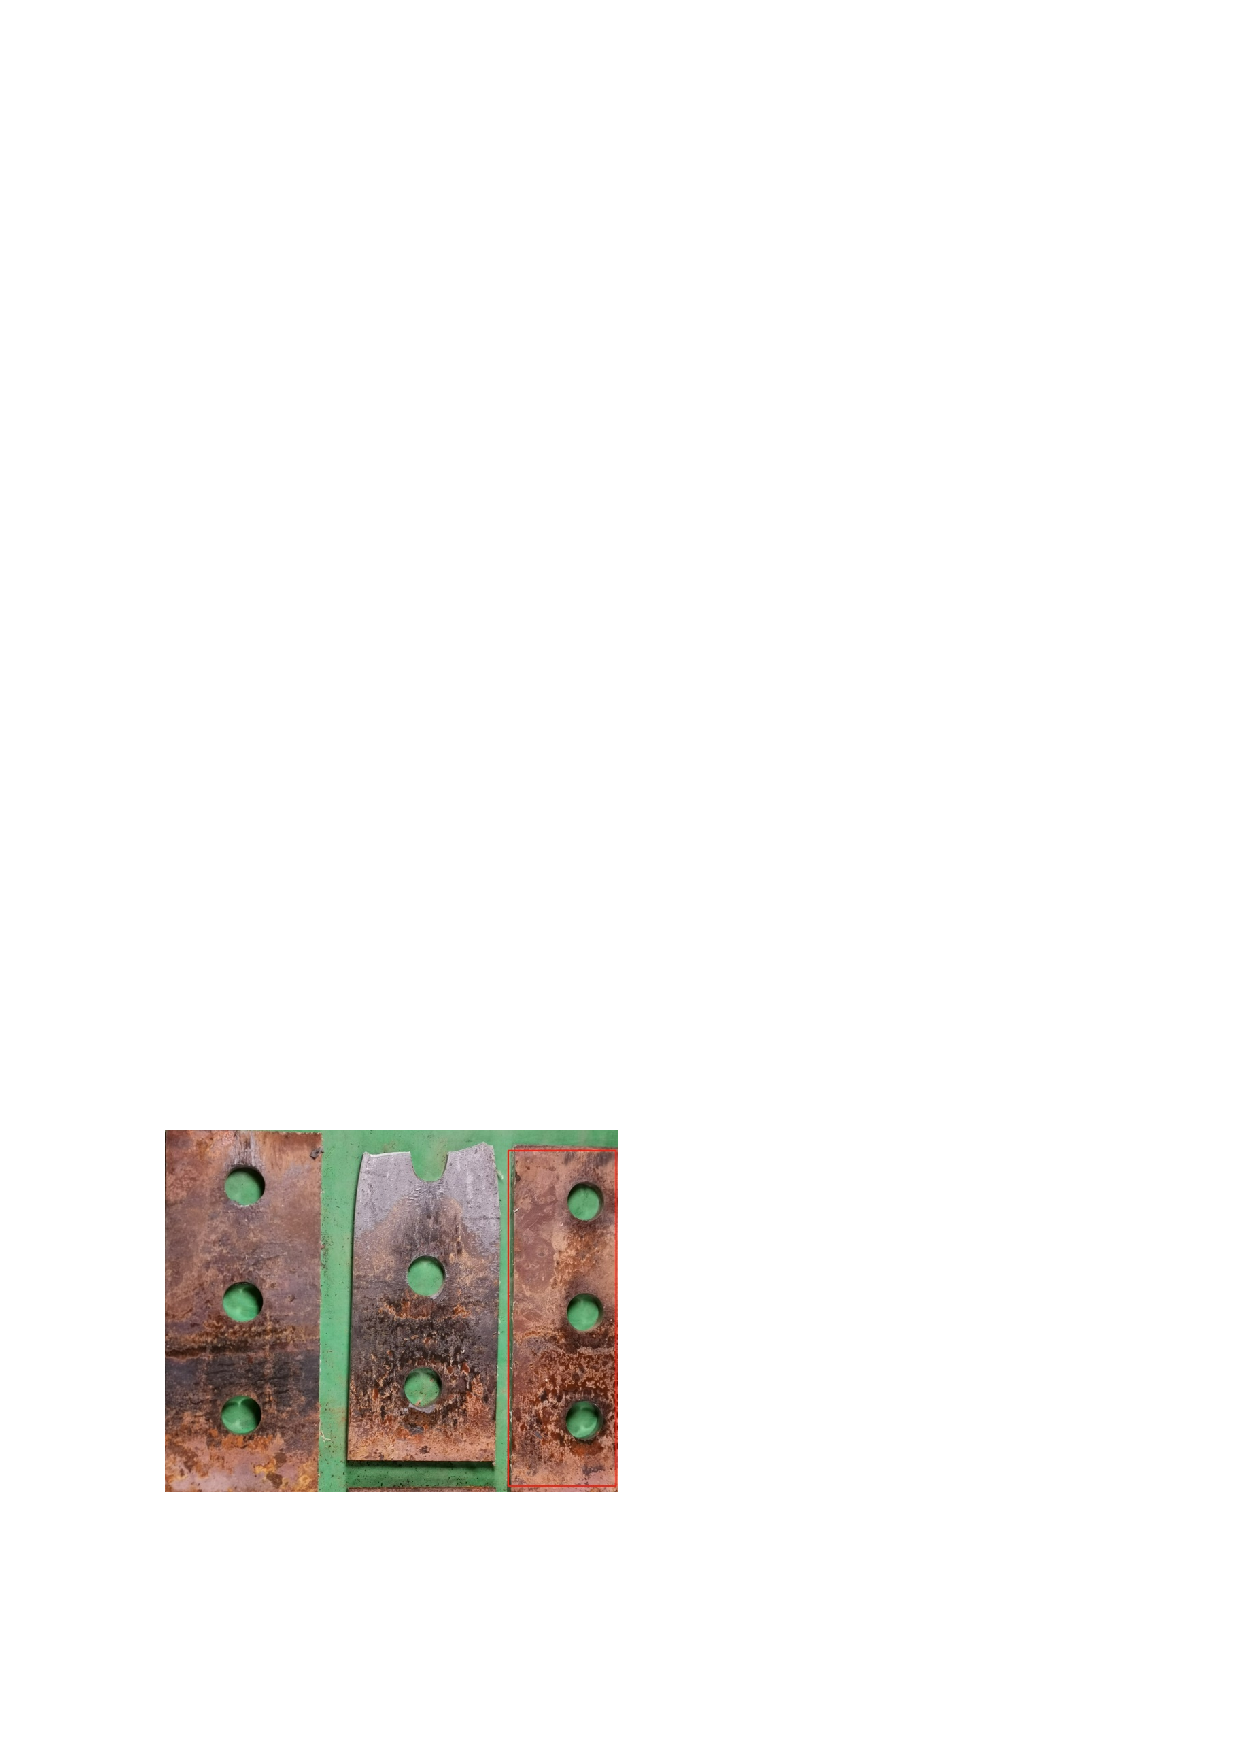
\includegraphics[width=\linewidth]{imgs/ch3/fig3-29.pdf}
    \caption{Enlarged view of the slip side}
    \label{fig3-29}
    \end{minipage}
    \begin{minipage}[t]{0.45\textwidth}
    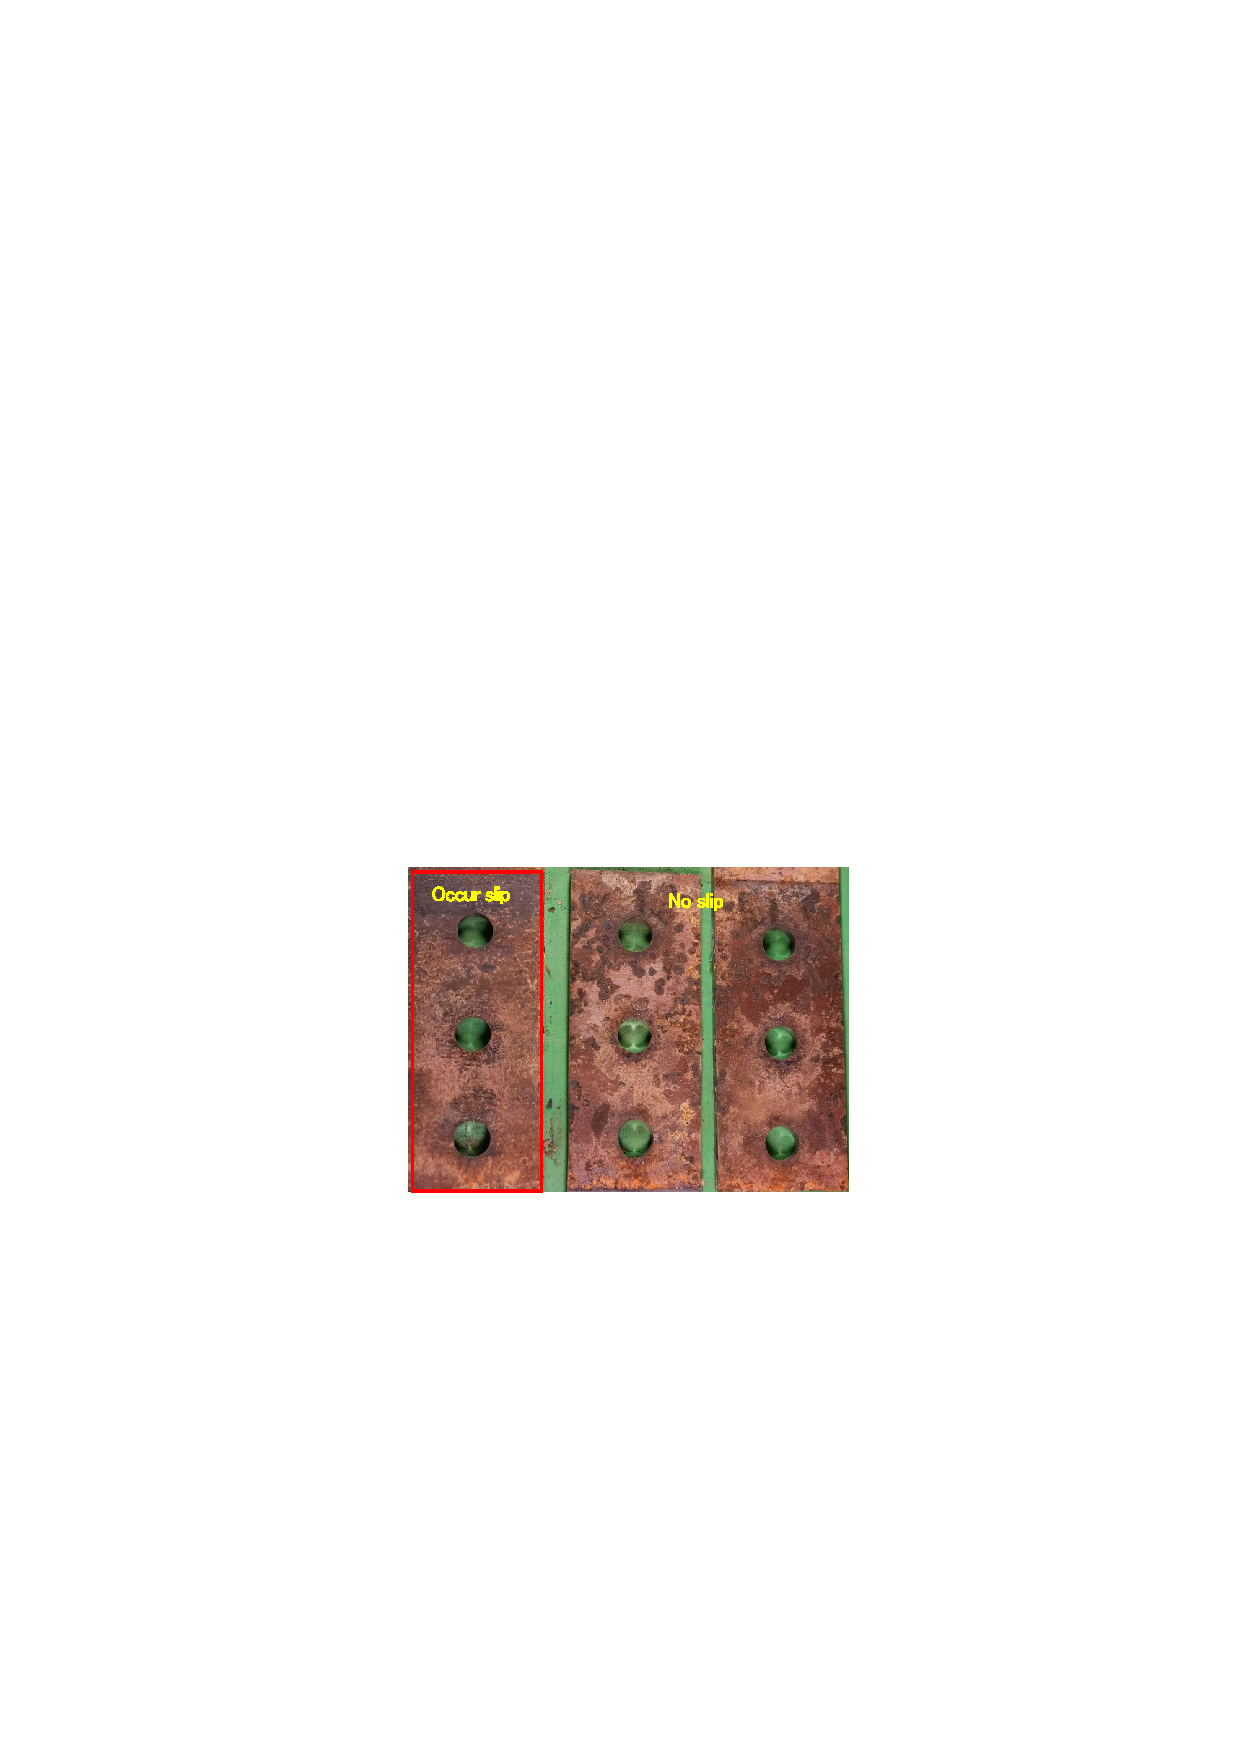
\includegraphics[width=\linewidth]{imgs/ch3/fig3-30.pdf}
    \caption{Enlarged view of the fixed side}
    \label{fig3-30}
    \end{minipage}
\end{figure} 





\section{Conclusions}

\textbf{For the slip coefficient of riveted joint }

In this chapter, the joint part cut out from a 90-year-old riveted bridge's cross-beam. It evaluated the riveted joint surface's aging condition with red lead by microscope observation and chemical analysis. The slip and pressure distribution tests are also conducted to investigate the joint surface's slip coefficient of the riveted joints and the pressure distribution of riveted joints' surface. 

Given the results of the present research, the obtained conclusions are as follows: 

\begin{itemize}
    \item The distribution of red lead on the joint surface is not flat, the adhesion of the red lead has deteriorated, and the black oxide on the surface of the steel can be observed. In addition to the red lead film, vinyl acetate was also discovered by the FT-IR spectra analysis. 

    \item The average slip coefficient was 0.274, and the coefficient of variation was 0.191.-2σ is 0.169. The 95\% confidence interval for the slip coefficient is 0.259-0.289. 

    \item According to the relationship between the slip coefficient and clamping force, it has been confirmed that the change of the clamping force will not affect the slip coefficient.

    \item The pressure distribution test could be concluded that due to the joint surface is not flat, the pressure distribution is also very uneven, and very high pressure is generated locally. On the contrary, there is no effective pressure applied in some places called an invalid contact area. Besides, the slip coefficient has no obvious relationship with effective contact pressures.
    
\end{itemize}

\textbf{for the tensile test of test of partially replacement of riveted joint}

The girth thicknesses of the joints cut from the transverse girders of the riveted bridge, which had been in service for 90 years, averaged 9.2 mm and 10.3 mm, respectively, which were different from the design value of 9.5 mm. This indicates that the level of steel plate manufacturing technology at that time was not very high. In addition, there were many impurities and inclusions in the steel material, and voids were found in the material specimens and girth joints. It is thought that lamination is somewhat common in steel structures due to aging, and the extent to which it affects the bearing capacity of the structure is also unknown.

In this study, tensile tests were conducted on existing riveted joints to determine the load carrying capacity of the joints when they were partially or fully replaced with high-strength bolts for friction joints, and the slip coefficient that can be expected in the design. The results of this study are as follows.

\begin{itemize}
    \item The bearing capacity of a riveted joint in a sound condition is about 1.4 times higher than the pure section yield capacity, and the joint is ahead of yielding. The tensile behavior of the riveted joint is as follows: first, slip occurs while the rivet is deformed, then the load rises to the bearing state, after which the pure section yields and the main plate enters a plastic state. Then, rupture of the main plate net section occurs. The frictional resistance caused by the axial force introduced during rivet cooling is smaller than the joint bearing capacity, and its effect is extremely small. Therefore, it is desirable to design the bearing capacity without considering the axial force introduced into the rivet as in the conventional design in the future.
    
    \item In the case of the yield-precedence type joint, almost the same bearing capacity was obtained when all the rivets were replaced with high-strength bolts and when only the rivets on the outside of the joint were replaced with high-strength bolts. Therefore, it is desirable to replace only the rivets on the outside of the joint for economic and workability reasons. In this experiment, an enlarged hole with a diameter of $\phi$ 26.5 mm was used to remove the rivets. The net cross-sectional yield strength of the specimen with the enlarged hole was 1.1 times that of the Rivet joint in its sound condition. The standard $\phi$ 24.5mm bolt hole diameter further increases the net sectional yield strength.
    
    \item When the main plate is of the yield-precedence type, the net sectional yield capacity depends on the frictional force per bolt on the outside of the joint. For a constant slip coefficient, the higher the axial force, the higher the rate of increase of the net sectional yield strength. When replacing rivets, introducing a higher axial force with a high-strength bolt is expected to improve the strength of the joint.
    
    \item In this experiment, the slip coefficients of the two contact surfaces on the fixed side of the specimen, which were all replaced with high-strength bolts, differed by a factor of approximately two, confirming the phenomenon that only one joint surface slides. In the future, it will be necessary to investigate cases where the slip coefficient differs between the two joint surfaces, since such a case is expected to occur in actual joints.
\end{itemize}